%% thesis.tex 2014/04/11
%
% Based on sample files of unknown authorship.
%
% The Current Maintainer of this work is Paul Vojta.
%
% https://math.berkeley.edu/~vojta/tex/ucbthesis-phd.html

\documentclass{ucbthesis}
\usepackage[dvipdfmx]{graphicx} % needs to be up top
\usepackage{bmpsize}
\usepackage{amsmath}
\usepackage{amssymb}
\usepackage[sorting=none,backend=biber]{biblatex}
\usepackage{color}
\usepackage{etoolbox}
\usepackage[hidelinks]{hyperref}
\usepackage[super]{nth}
\usepackage{tikz}
\usepackage{tikz-3dplot}
\usetikzlibrary{arrows}
\usetikzlibrary{decorations.pathreplacing}
\usetikzlibrary{3d,angles,quotes,calc}
\usepackage[export]{adjustbox} % must be below tikz else tikzplots are scronched
\usepackage[version=3]{mhchem}
\usepackage{textcomp}
\usepackage{stmaryrd} % for short right arrow
\usepackage{placeins}
\usepackage{multirow}
\usepackage{subcaption}

\newcommand{\sa}{\shortrightarrow}
\newcommand{\bo}{\mathbf\Omega}
\newcommand{\vecr}{\textbf{r}}
\newcommand{\sn}{S$_\mathrm{N}$~}
\newcommand{\pn}{P$_\mathrm{N}$~}
\newcommand{\sigt}{\Sigma_t}
\newcommand{\sigs}{\Sigma_s}
\newcommand{\hl}{\mathcal{H}_L}
\newcommand{\maths}{\mathbb{S}^2}
\newcommand{\dl}{d_L}
\newcommand{\lij}{\langle L_i,L_j \rangle}
\newcommand{\kij}{\langle K_i,K_j \rangle}
\newcommand{\ve}[1]{\ensuremath{\mathbf{#1}}}
\newcommand{\Ye}[2]{\ensuremath{Y^e_{#1}(\bo_#2)}}
\newcommand{\Yo}[2]{\ensuremath{Y^o_{#1}(\bo_#2)}}
\newcommand{\Sigg}[1]{\ensuremath{\Sigma^{g'\sa g}_{\text{s},#1}}}
\newcommand{\even}{\ensuremath{\phi^g}}
\newcommand{\odd}{\ensuremath{\vartheta^g}}
\newcommand{\xhat}{\ensuremath{\hat{x}}}
\newcommand{\xbar}{\ensuremath{\bar{x}}}
\newcommand{\qhat}{\ensuremath{\hat{q}}}
\newcommand{\psihat}{\ensuremath{\hat{\psi}}}
\newcommand{\khat}{\ensuremath{\hat{K}}}
\newcommand{\Gij}[2]{\sum_{\ell=0}^L\frac{2\ell+1}{4\pi}P_{\ell}(\bo_#1\cdot\bo_#2)}
\newcommand{\Sij}[2]{\Sigma^{g'\rightarrow g}_{\text{s,L}}(\bo_#1\cdot\bo_#2)}
\newcommand{\Snij}[3]{\Sigma^{g'\rightarrow g}_{\text{s,#1}}(\bo_#2 \cdot \bo_#3)}
\newcommand{\Snz}[3]{\Sigma^{0\sa 0}_{\text{s,#1}}(\bo_#2 \cdot \bo_#3)}
\newcommand{\ldosig}[2]{\sum_{n=0}^N \frac{2n+1}{4\pi}\sigma_{s,n}^{g'\rightarrow g} P_n(\bo_#1\cdot\bo_#2)}
\newcommand{\fq}{\qquad\qquad\qquad\qquad}
\newcommand{\st}{\tilde{S}}
\newcommand{\E}[1]{$\times10^{#1}$}
\newcommand{\del}{\partial}
\newcommand{\mr}[1]{\multirow{2}{*}{#1}}

\makeatletter
\let\oldcite\cite
\pretocmd{\listoffigures}{\def\cite{\ignorespaces\@gobble}}{}{}
\apptocmd{\listoffigures}{\let\cite\oldcite}{}{}
\makeatother

\makeatletter
\let\oldcite\cite
\pretocmd{\listoftables}{\def\cite{\ignorespaces\@gobble}}{}{}
\apptocmd{\listoftables}{\let\cite\oldcite}{}{}
\makeatother

% To compile this file, run "latex thesis", then "biber thesis"
% (or "bibtex thesis", if the output from latex asks for that instead),
% and then "latex thesis" (without the quotes in each case).

% Double spacing, if you want it.  Do not use for the final copy.
% \def\dsp{\def\baselinestretch{2.0}\large\normalsize}
% \dsp

% If the Grad. Division insists that the first paragraph of a section
% be indented (like the others), then include this line:
% \usepackage{indentfirst}

\newtheorem{theorem}{Jibberish}

\bibliography{references}

\hyphenation{mar-gin-al-ia}
\hyphenation{bra-va-do}
\hyphenation{quad-ru-ple}
\hyphenation{ADVANTG}
\hyphenation{CADIS}
\newcommand{\fwc}{\mbox{FW-CADIS}}
\newcommand{\co}{\mbox{CADIS-$\Omega$}}
\newcommand{\fwco}{\mbox{FW/CADIS-$\Omega$}}

\begin{document}

% Declarations for Front Matter

\title{Advanced Quadrature Selection for Monte Carlo Variance Reduction}
\author{Kelly L. Rowland}
\degreesemester{Spring}
\degreeyear{2018}
\degree{Doctor of Philosophy}
\chair{Assistant Professor Rachel N. Slaybaugh}
\othermembers{
	Associate Professor Per-Olof Persson \\
	Professor Jasmina Vuji\'c \\
	Dr. Steven P. Hamilton
	}
\numberofmembers{4}
\field{Engineering -- Nuclear Engineering}
% Designated Emphasis -- this is optional, and rare
\emphasis{Computational and Data Science and Engineering}
\campus{Berkeley}

\maketitle
% Delete (or comment out) the \approvalpage line for the final version.
% \approvalpage
\copyrightpage

% (This file is included by thesis.tex; you do not latex it by itself.)

\begin{abstract}

Neutral particle radiation transport simulations are critical for radiation shielding and deep
penetration applications. Arriving at a solution for a given response of interest can be 
computationally difficult because of the magnitude of particle attenuation often seen in these 
shielding problems. Hybrid methods, which aim to synergize the individual favorable aspects of
deterministic and stochastic solution methods for solving the steady-state neutron transport
equation, are commonly used in radiation shielding applications to achieve statistically
meaningful results in a reduced amount of computational time and effort. The current state of the
art in hybrid calculations is the Consistent Adjoint-Driven Importance Sampling (CADIS) and 
Forward-Weighted CADIS (\fwc) methods, which generate Monte Carlo variance reduction parameters
based on deterministically-calculated scalar flux solutions. For certain types of radiation
shielding problems, however, results produced using these methods suffer from unphysical
oscillations in scalar flux solutions that are a product of angular discretization. These 
aberrations are termed ``ray effects''.

The Lagrange Discrete Ordinates (LDO) equations retain the formal structure of the traditional
discrete ordinates formulation of the neutron transport equation and mitigate ray effects at high
angular resolution. In this work, the LDO equations have been implemented in the Exnihilo parallel
neutral particle radiation transport framework, with the deterministic scalar flux solutions
passed to the Automated Variance Reduction Generator (ADVANTG) software and the resultant Monte
Carlo variance reduction parameters' efficacy assessed based on results from MCNP5. Studies were 
conducted in both the CADIS and \fwc\ contexts, with the LDO equations' variance reduction
parameters seeing their best performance in the \fwc\ method, especially for photon transport.

\end{abstract}


\begin{frontmatter}

% You can delete the \clearpage lines if you don't want these to start on
% separate pages.

\setcounter{secnumdepth}{3}
\setcounter{tocdepth}{3}

% to show paragraphs in ToC (good for an outline, stylistically ugly):
% \setcounter{secnumdepth}{4}
% \setcounter{tocdepth}{4}

\tableofcontents
\clearpage
\listoffigures
\clearpage
\listoftables

\begin{acknowledgements}
\small
It takes a village to make a doctor. I cannot express how grateful I am to
the colleagues, friends, family, and various community members who have
supported me throughout my tenure in graduate school. Without all of your
contributions, this process would have been much more difficult.

Many thanks go to my dissertation committee for their time and effort spent
in improving the quality of this writing. I would like to thank the Exnihilo
team at Oak Ridge National Laboratory for all of their help and guidance.
Dr. Steven Hamilton, you have my sincerest gratitude for your help at all
levels of this project, from working through big conceptual questions to
kindly pointing out the smallest of floating point errors. This work would
not have been finished in any sort of timely manner without your generosity.

My colleagues have made Berkeley an amazing place to work and grow. Drs.
Phil Gorman and Katy Huff, thank you for your patience and kindness in
teaching me scientific computing skills when I had none. Dr. Madicken Munk,
my commiserator-in-chief, thank you for seeing me through the most trying
of times and for paving a better-informed \texttt{PATH} than I would have
otherwise traversed. Daniel Wooten, thank you for helping me to say no
to more things. Josh Rehak, thanks for helping me keep it surreal. Ellen
Edwards, thank you for continually inspiring me to challenge myself.

Berkeley Research Computing has been a great source of pride and joy for me
to be a part of. Aaron Culich, I cannot thank you enough for looking at a
graduate student in desperate need of help and seeing the potential for so
much more. I am grateful to the Department of Nuclear Engineering for all of
the free coffee that it has provided.

To my family, thank you for your endless support and encouragement. You have
provided me with an incredible foundation from which I have been fortunate
to pursue any and all of my dreams.

Cathy Berman, thank you for being my personal cheerleader and helping me
grow into myself. Dr. Dillon Shaver, thank you for helping me pass my
screening exams when I really needed it.
Shola Ogunlana, thank you for leading the STRONGER family
to be better versions of ourselves through each and every burpee. Mitch
Crispell, thank you for bringing joy to every single person who steps into
one of your dance classes. Alex Converse, thank you for the love and support
that you have provided, even when it meant bearing with me through a few
periods of crunch time.

Professor Rachel N. Slaybaugh, thank you for advising me in so much more
than just this dissertation work. Your perspective and insights have helped
me to not only bloom as a researcher, but to a grow as a person as well. I
am very fortunate to have had your support in the myriad of endeavors that
I have undertaken in graduate school. Thank you for caring about my well-being
as an individual and broadening my horizons in ways that I never could have
fathomed.

\vspace{\fill}

\scriptsize{This material is based upon work supported under an Integrated
University Program Graduate Fellowship as well as supported by the Department 
of Energy under Award Number(s) DE-NE0008661. This report was prepared as an account 
of work sponsored by an agency of the United States Government. Neither the United 
States Government nor any agency thereof, nor any of their employees, makes any 
warranty, express or limited, or assumes any legal liability or responsibility for the 
accuracy, completeness, or usefulness of any information, apparatus, product, or
process disclosed, or represents that its use would not infringe privately owned
rights. Reference herein to any specific commercial product, process, or service by
trade name, trademark, manufacturer, or otherwise does not necessarily constitute or
imply its endorsement, recommendation, or favoring by the United States Government or
any agency thereof. The views and opinions of authors expressed herein do not 
necessarily state or reflect those of the United States Government or any agency 
thereof. This research used the Savio computational cluster resource provided by the 
Berkeley Research Computing program at the University of California, Berkeley 
(supported by the UC Berkeley Chancellor, Vice Chancellor for Research, and Chief 
Information Officer).}

\end{acknowledgements}

\end{frontmatter}

\pagestyle{headings}

% (Optional) \part{First Part}

\chapter{Introduction}

The work covered in this dissertation includes the implementation of the Lagrange 
Discrete Ordinates (LDO) equations in the Exnihilo parallel neutral particle radiation 
transport framework for the purpose of using the equations' solutions in Monte Carlo
variance reduction parameter generation via the ADVANTG software to improve the results of
simulations run with MCNP5. We start with an analysis of deterministic 
scalar flux results from solving the LDO equations
compared against those of standard discrete ordinates quadrature set types because the 
LDO equations have never before been implemented in a framework such as Exnihilo. Then,
we assess the performance of the Monte Carlo variance reduction parameters generated 
based on the forward and adjoint solutions from the various quadrature set types in the contexts
of both the Consistent Adjoint-Driven Importance Sampling (CADIS) and the Forward-Weighted 
CADIS (\fwc) methods.

\section{Motivation}

Radiation shielding is an important and interesting problem from various perspectives.
Simulation of shielding scenarios is critical for health physics and nuclear security
applications, but arriving at a solution for a given response of interest (e.g., 
neutron flux at a given location) can be computationally difficult in the context of
the magnitude of particle attenuation often seen in shielding problems.

The steady-state neutron transport equation (NTE), introduced below in Section
\ref{sec:nte}, is typically solved using either deterministic methods or stochastic
(Monte Carlo) methods. We will look at each of these solution methods in further 
detail in Chapter \ref{bgch}, but briefly note here that both solution methods have
individual strengths and weaknesses. So-called ``hybrid'' methods aim to combine the
favorable aspects of deterministic and Monte Carlo methods to achieve better results.
Although hybrid methods are used to significant effect in radiation shielding problems,
they do not entirely mitigate the negative aspects of the combined simulation types.

One particular area of study where hybrid methods tend to fall short is in shielding
problems with highly anisotropic particle movement and particle streaming pathways.
This is because the standard implementation of the CADIS and \fwc\ methods is based on scalar
particle flux rather than angular particle flux. So, solutions from deterministic calculations
exclude information about how particles move toward a response of interest.
For problems with strong anisotropies in the particle flux, the importance map and biased source 
developed using the standard space/energy treatment may not represent the real importance well 
enough to sufficiently improve efficiency in the Monte Carlo calculation. 

This work aims to gauge the performance of Monte Carlo biasing parameters based on
scalar flux solutions from solving the LDO equations. We will be employing the LDO equations'
solutions in the standard CADIS and \fwc\ methods to assess how well the LDO representation's
unique treatment of scattering and asymmetry in angle incorporate angular information into the
resultant scalar flux solutions and corresponding Monte Carlo biasing parameters.

\section{Goals and Impacts}
\label{goals}

The primary goal of this work is to assess the forward and adjoint scalar flux 
solutions of the Lagrange Discrete Ordinates equations as input for Monte Carlo 
variance reduction parameter generation in the contexts of the CADIS and \fwc\ methods.
Additional research objectives in support of the primary goal for this work include:

\begin{itemize}
\item{Implement the LDO equations in a neutral particle radiation transport framework 
      designed to solve the traditional discrete ordinates form of the NTE.}
\item{Choose a small variety of test cases in which to assess the various quadrature
      types' deterministic scalar flux solutions for efficacy in Monte Carlo variance reduction 
      parameter generation.}
\item{Compare forward and adjoint scalar flux solutions resultant from the LDO
      equations against those generated with standard discrete ordinates quadrature
      sets for the chosen test scenarios.}
\item{Test the impact of biasing parameters' angular mesh refinement on Monte Carlo results
      across various quadrature types.}
\end{itemize}

\noindent In meeting these objectives as progress towards accomplishing the primary research goal,
we verify the relative accuracy of the deterministic solutions of the LDO equations and then 
examine how they perform as the deterministic solver for hybrid methods. The test problems used 
are those that challenge hybrid methods in general, and so we have generated
a variety of results of interest to the community at large.

\section{The Neutron Transport Equation}
\label{sec:nte}

The way in which neutrons move, known as ``neutron transport", is governed by the
time-dependent neutron transport equation (NTE) \cite{dude}:

\begin{multline}
\frac{1}{v}\frac{\del}{\del t}\psi(\vecr,E,\bo,t) +  \bo \cdot \nabla \psi(\vecr,E,\bo,t) + 
\Sigma_t(\vecr,E) \psi(\vecr,E,\bo,t) =  \\
\int_0^\infty\int_{4\pi} \Sigma_s(\vecr,E'\rightarrow E,\bo'\cdot\bo)
\psi(\vecr,E',\bo',t)d\bo'dE' + Q(\vecr,E,\bo,t),
\label{eq:tnte}
\end{multline}

\noindent where $\vecr$ is the neutron position, $E$ is the energy of the neutron,
$\bo$ is the direction of travel of the neutron, and $t$ is the time. The combination of 
$(\vecr,E,\bo,t)$ is generally referred to as the ``phase space'' of the particles. $\psi$ 
denotes angular neutron flux, $\Sigma$ represents the cross section of a material, and $Q$ is
any additional source (fission, a fixed source, etc.) of neutrons.

We are often interested in situations in which the particle flux is not a function of time. In
these cases, we solve the time-independent (steady-state) neutron transport equation, written as

\begin{multline}
\bo \cdot \nabla \psi(\vecr,E,\bo) + \Sigma_t(\vecr,E) \psi(\vecr,E,\bo) =  \\
\int_0^\infty\int_{4\pi} \Sigma_s(\vecr,E'\rightarrow E,\bo'\cdot\bo)
\psi(\vecr,E',\bo')d\bo'dE' + Q(\vecr,E,\bo).
\label{eq:nte}
\end{multline}

The steady-state neutron transport equation can be thought of as a balance equation in 
which the neutron losses represented on the left-hand side of the equation are equal to
the neutron gains represented on the right-hand side of the equation \cite{dude}. The 
first term on the left-hand side of the steady-state NTE accounts for all neutrons lost by 
streaming out through the surface of the system being considered. The second term in 
the left-hand side of the steady-state NTE accounts for all neutrons 
lost to collisions; this includes neutrons lost via absorption as well as neutrons that
exit the phase space of interest by scattering into a different energy and angle. The 
right-hand side of the equation totals system gains by summing up all neutrons that 
scatter into the phase space of interest from different energies and angles along with 
neutrons created from the source. The scattering term depends not on the individual
angles $\bo$ and $\bo'$ but on their dot product.

The derivative in the first term of the steady-state NTE suggests that we must prescribe 
appropriate boundary conditions for the equation in order to solve the problem. The boundary
conditions depend on the given problem of interest and will be discussed in more detail later.
The following chapter will provide in-depth explanations of various solution methods 
for the time-independent NTE.

\section{Dissertation Outline}

The remainder of this dissertation is structured so as to provide a relevant theoretical
background and discussion as a prelude to the eventual presentation of the results and analysis
arrived at in meeting the sundry and ultimate objectives listed above in Section \ref{goals}.
Chapter \ref{bgch} provides a theoretical basis of the foundation of solution methods for the
NTE, followed by a discussion of pertinent work in the area of hybrid methods. Specific attention
is given to developments that aimed to incorporate angular information into Monte Carlo biasing
parameters; we will see in Section \ref{sec:ldo} that the interest in using the LDO equations'
solutions for Monte Carlo variance reduction parameter generation stems from the unique way in
which the LDO equations treat particle scattering.

Transitioning from theory to practice, Chapter \ref{ch:method} examines the
traditional discrete ordinates equations and the LDO equations from the
perspective of implementing both sets of  equations in a neutral particle
radiation transport software framework. Specific focus is given on the
differences in implementing the contrasting equations; a discussion of details
regarding the solution of the LDO equations in a framework designed to solve the
conventional discrete ordinates equations concludes the chapter.  We note that
the discussion in Chapters \ref{bgch} and \ref{ch:method} focuses on neutron
transport, but the solution methods can be leveraged for photon transport as
well; Chapter \ref{sec:results} presents the test case scenarios examined in
this work with results from the various hybrid methodologies for both neutron
and photon transport problems. Chapter  \ref{ch:conc} concludes the dissertation
with a summary review of the results and  analysis followed by a brief
discussion of future work paths.

\chapter{Background}
\label{bgch}

This chapter provides information relevant to the core parts of this research, with 
a particular focus on areas relevant to the novel work presented. We start by 
discussing the two main approaches to solving the NTE, Monte Carlo methods and 
deterministic methods, as the hybrid methods that are described next incorporate both
types of solutions. Then, a discussion of previous work in the field of hybrid methods
is given, with a specific focus on the CADIS method and variants on that method as
well as significant historical work that has incorporated angular information into
hybrid methods. Finally, we present a mathematical background for and derivation of 
the LDO equations.

\section{Approaches to Solving the Neutron Transport Equation}

\subsection{Monte Carlo Methods}

Solving the NTE using Monte Carlo methods approximates ``following'' the individual
particles from birth to death. The purpose of particle tracking is to calculate the
expectation or mean value $\xbar$ of some quantity of interest, often the neutron 
scalar flux. The estimate of this quantity takes the form of the average of $N$ 
samples:

\begin{equation}
\xhat = \frac{1}{N}\sum_{n=1}^{N}x_n,
\end{equation}

\noindent where $x_n$ is the contribution from the $n^{th}$ particle history to the
quantity of interest.
As the calculation proceeds, $x_n$ is tallied from each neutron history in order 
to calculate the estimated or sample mean $\xhat$ at the end of the calculation.
Errors in Monte Carlo calculations take the form of stochastic uncertainties, as the 
independent variables of the NTE are treated continuously. Taking this into
consideration, it is useful to quantify how good of an estimate the sample value
$\xhat$ is to the true mean value $\xbar$.

For some property of a Monte Carlo history $x$ sampled from a continuous probability density 
function $f(x)$, the variance of that property is defined to be

\begin{equation}
\sigma^2(x) = \overline{x^2} - \xbar^2,
\end{equation}

\noindent where

\begin{equation}
\overline{x^n} \equiv\int_{-\infty}^{\infty}x^n f(x)dx.
\end{equation}

The standard deviation of the property is calculated as the square root of the
variance:

\begin{equation}
\sigma(x) = \left(\overline{x^2} - \xbar^2\right)^{1/2}
\end{equation}

\noindent and provides a measure of the spread of $x$ about the mean value $\xbar$
\cite{lm}. With this, the variance and standard deviation of $\xhat$ can be 
expressed in terms of the variance and standard deviation of $x$ as

\begin{equation}
\sigma^2(\xhat) = \frac{1}{N}\sigma^2(x)
\end{equation}

\noindent and

\begin{equation}
\label{eq:mc_var}
\sigma(\xhat) = \frac{\sigma(x)}{\sqrt{N}}, 
\end{equation}

\noindent respectively. A low standard deviation indicates that the values of $x$ are 
closely clustered near $\xbar$, while a high standard deviation indicates a large 
spread in the values of $x$. If $\xhat$, constructed from $N$ values of $x_n$, is
used to estimate $\xbar$, then the spread in the results of $\xhat$ about $\xbar$
is proportional to $\sigma(x)$ and falls off as the square root of the number of 
histories in the sample, as seen in Equation \ref{eq:mc_var} \cite{lm}. This is to 
say, generally, that a greater number of histories contributing to the property of 
interest being calculated results in a lower standard deviation of the estimate of 
that property.

For a given Monte Carlo calculation, the sample variance is defined as

\begin{equation}
S^2 = \frac{1}{N-1}\sum_{n=1}^{N}\left(x_n - \xhat\right)^2
\end{equation}

\noindent and is considered to be an unbiased estimator of the variance; the 
expectation value of the sample variance is equal to the variance, $\sigma^2(x)$ 
\cite{lm}. Because it is an unbiased estimator of the variance, the sample variance
allows us to estimate the spread in $\xhat$; this is useful because $\xhat$ is the
value that actually results from the Monte Carlo calculation. In practice, the sample
variance and standard deviation are calculated as

\begin{equation}
S^2 = \frac{N}{N-1}\left(\widehat{x^2} - \xhat^2\right), \text{ where }
\widehat{x^2} \equiv \frac{1}{N}\sum_{n=1}^{N}x_n^2,
\end{equation}

\noindent and

\begin{equation}
S = \left(\frac{N}{N-1}\right)^{1/2}
\left[\frac{1}{N}\sum_{n=1}^{N}x_n^2 - \xhat^2\right]^{1/2},
\end{equation}

\noindent respectively \cite{lm}. For large numbers of histories, $\frac{N}{N-1}$ is 
often set equal to one.

The simplest Monte Carlo model for particle transport problems is the ``analog''
model that uses the real probability that various events occur \cite{mcnp}. In the
analog model, particles are followed from event to event, and the next event is 
always sampled from a number of possible events according to the real event 
probabilities. This is called the analog Monte Carlo model because it is directly 
analogous to the naturally occurring transport; it works well when a significant
fraction of the particles contribute to the tally estimate and can be compared to
detecting a significant fraction of the particles in the physical situation.

To quantify the efficiency of calculating a given quantity of interest, a metric known
as the ``figure of merit'' is often used.

\subsubsection{The Figure of Merit}

The figure of merit (FOM) is defined as

\begin{equation}
\text{FOM} = \frac{1}{R^2T},
\label{eq:fom}
\end{equation}

\noindent where $R$ is the estimated relative error, defined as $S/\xhat$, and $T$ is
the computer time taken to complete the calculation \cite{mcnp}. This value should be 
approximately constant for any one Monte Carlo calculation, as $R^2$ is 
proportional to $1/N$ and $T$ should be directly proportional to $N$.

As stated earlier, estimates for quantities of interest with the lowest statistical error
are usually obtained for quantities to which a substantial fraction of the histories 
contribute. That is to say, in order to get estimates for quantities of interest that 
are statistically meaningful (have sufficiently low statistical error), a sizable number of 
the particle histories tracked should contribute to the estimate. This can be 
difficult to achieve in a reasonable amount of computational time for certain analog 
Monte Carlo calculations. That is to say, if these analog calculations were allowed 
to continue until convergence, they would have a very small FOM because of the sheer
amount of calculation time needed for the calculation to finish. A pertinent example 
of this type of problem is a neutron shielding scenario, in which the neutron scalar 
flux varies by orders of magnitude through the shield and over the problem geometry. 
In these cases, ``non-analog'' techniques are introduced.

Non-analog Monte Carlo attempts to follow ``interesting'' particles more often 
than uninteresting ones, where an interesting particle is one that contributes much more
to the quantity that needs to be estimated. Non-analog techniques are 
meant to increase the odds that a given particle contributes to the quantity of
interest. To ensure that the average score is the same in the non-analog model as in 
the analog model, the score is modified to remove the effect of biasing the natural 
odds.

A non-analog Monte Carlo technique will have the same expected tallies as an 
analog technique if the expected weight executing any given random walk is preserved.
These variance reduction techniques can often decrease the relative error by 
sampling naturally rare events with an unnaturally high frequency and weighting the 
tallies appropriately. In the following subsection, several variance reduction methods
are described and discussed.

\subsubsection{Variance Reduction}

Commonly used classes of variance reduction techniques are truncation methods,
population control methods, and modified sampling methods \cite{mcnp}.
Some variance reduction methods are generally applicable, while others are more 
specialized and carry high risk in use. Some variance reduction techniques cause an 
increase in computational time, but variance typically decreases faster than 
the increase in time, so these techniques still result in a net increase of the FOM
\cite{olsher}.

\paragraph{Truncation Methods}\mbox{} \\

Of the classes listed above, truncation methods are the simplest; they aim to 
accelerate
calculations by truncating parts of phase space that do not contribute significantly 
to the problem solution. One example of this is geometry truncation, in which 
unimportant parts of the problem geometry are not modeled. Truncation methods may 
also be applied to other independent variables such as energy; when using
energy cutoff, particles whose energy is out of the range of interest are terminated 
so that computation time is not spent following them.

\paragraph{Population Control Methods}\mbox{} \\

Population control methods use particle splitting and Russian roulette to control the 
number of samples taken in various regions of phase space. In important regions, many
samples of low weight particles are tracked, and in unimportant regions, few samples 
of high weight are tracked. Weight adjustments are made to the particles to ensure 
that the problem solution remains unbiased. Specific population control methods 
include geometry splitting and Russian roulette, energy splitting and roulette, 
weight cutoff, and weight windows \cite{mcnp}.

Using geometry splitting with Russian roulette, particles transported from a region 
of higher importance to a region of lower importance undergo Russian roulette. Some 
of the particles will be killed a certain fraction of the time, but survivors will be 
counted more by increasing their weight the remaining fraction of the time. In doing
this, unimportant particles are followed less often, yet the problem solution remains 
undistorted. If a particle is transported to a region of higher importance, it may be 
split into two or more particles, each with less weight and therefore counting less. 
In this case, important particles are followed more often, yet the solution is again 
undistorted because, on average, the total weight is conserved.

In general, when a particle of weight $w_0$ is split into $k$ particles, the resulting
particles are each given a weight of $\frac{w_0}{k}$, conserving the expected 
weight. When a particle is subject to Russian rouletting, it is turned into a 
particle of weight $w_1 > w_0$ with probability $\frac{w_0}{w_1}$ and is killed with 
probability $1 - \frac{w_0}{w_1}$, again conserving the expected weight.

Geometry splitting with Russian roulette can be used to great advantage in deep
penetration shielding problems. Splitting helps maintain the particle population, 
which diminishes rapidly in analog simulations. Conversely, geometry splitting with 
Russian roulette does not work well in problems that have severe angular dependence. 
In the most extremely anisotropic case, a particle may never enter a geometric region 
in which it may be split \cite{mcnp}.

Energy splitting and Russian roulette are generally used in combination but may be
employed separately. When using energy splitting, once a neutron drops below a given
energy threshold, it may be split into multiple neutrons, each with an appropriately
adjusted weight. This is useful when particles are more important in some energy 
ranges than in others. In the case of using energy rouletting, if a particle drops 
below a certain energy, a roulette game is played and the particle is either killed 
or survives with a weight increased by a factor of the reciprocal of the survival 
probability (to conserve overall particle population weight). These two energy-based 
variance reduction techniques are independent of spatial location, so a space-energy 
weight window (discussed below) is usually a better choice for problems with strong 
space-energy dependence.

When weight cutoff is employed, Russian roulette is played if a particle's weight 
drops below a specified cutoff value. The result of the roulette is that the particle 
is either killed or survives with its weight increased to a given level. Weight 
cutoff is most efficient when used in combination with geometry splitting (discussed 
above) and implicit capture (discussed below). It is important to note that, unlike 
in the case of the energy cutoff, the weight cutoff does not bias the solution 
because the particles that survive do so with increased weight.

The last population control method discussed here is the weight window, which is a 
phase space splitting and Russian roulette technique. The phase space may be 
space-energy or solely space.
Each phase space cell is bounded by upper and lower weight bounds. If a particle is
above the upper weight bound, it is split such that the resultant particles are all
within the bounds of the weight window. If a particle is below the lower weight bound,
Russian roulette is played and the particle is either terminated or permitted to
survive with an increased weight within the bounds of the weight window. If a 
particle's weight is within the window, no action is taken. All of these scenarios are
depicted in Figure \ref{fig:ww}, a cartoon of the weight window concept.

\begin{figure}[!htb]
\centering
\includegraphics[width=0.85\textwidth]{img/ww-mcnp.eps}
\caption{Weight window phase space splitting and Russian roulette \cite{mcnp}.}
\label{fig:ww}
\end{figure}

The weight window may be used alone to good effect, but it is particularly powerful
when used in conjunction with other variance reduction techniques that introduce large
variations in particle weight. Well-specified weight windows keep the Monte Carlo 
solution from severe perturbations resulting from high-weight particles and 
simultaneously keep computational resources from wasting time on low-weight particles
by rouletting them.

\paragraph{Modified Sampling Methods}\mbox{} \\

Modified sampling methods alter the statistical sampling of a problem to increase the 
number of tallies per particle. For a given Monte Carlo event, it is possible to 
sample from an arbitrary distribution rather than the physical probability as long as 
the particle weights are adjusted to compensate. With modified sampling methods, 
sampling is done from distributions that send particles in desired directions or into 
other desired regions of phase space such as time or energy. Modified sampling methods
may also change the location or type of collisions. Categories of modified sampling
methods include implicit capture, forced collisions, and source biasing.

Using implicit capture (also called implicit absorption or survival biasing), 
particles are never killed by absorption. Instead, a particle's weight is reduced by
the absorption probability at each collision, allowing important particles to
survive by not being lost to absorption. Implicit capture can be thought of as a 
splitting process in which a particle of weight $w_0$ is split into two particles: one
of weight $w_0(1-\frac{\Sigma_a}{\Sigma_t})$ that survives and is 
subsequently followed, and one of weight $w_0\frac{\Sigma_a}{\Sigma_t}$ that is
instantaneously killed \cite{mcnp}.

The forced collision method increases sampling of collisions in specified spatial 
cells. Particles undergoing forced collisions are split into collided and uncollided
parts. The collided part of the particle is forced to react within the current cell,
while the uncollided part of the particle exits the cell without collision. When the
track of the uncollided particle portion is continued, it is followed with weight
$w_0e^{-\Sigma_t d}$, where $w_0$ is the original particle weight and $d$ is the
distance traveled between the splitting site and the cell boundary. The collided part
of the particle thus reacts with weight $w_0\left(1 - e^{-\Sigma_t d}\right)$. These
resultant weights are chosen to reflect the actual physics of the problem; 
$e^{-\Sigma_t d}$ is the probability of exiting the cell without collision, and 
$1 - e^{-\Sigma_t d}$ is the probability of colliding in the cell. One of these two
things must happen to the original particle of weight $w_0$, so we observe that the starting
weight is preserved.

Finally, particle sources may be biased with respect to one or more variables. This
allows for greater numbers of particles to be produced in more important ranges of 
each biased variable, with the particles' weights reduced accordingly. In the relevant
example of the neutron shielding problem, one may start more particles
at high energies and in strategic directions in order to get more particles to 
contribute to the desired solution. The corresponding weights of the particles are 
altered to correct the statistical distribution.

\subsection{Deterministic Methods}

In the case of deterministic methods, each of the six independent variables of the 
steady-state NTE is discretized, relevant boundary conditions are imposed, and the 
resulting system of linear algebraic equations is iterated over until an acceptable
solution has been reached. We limit the discussion here to the discretization of the
integro-differential form of the NTE and the finite-volume discrete ordinates method.

These discretizations introduce some errors into the calculations, with the
discretization of some variables being more problematic than others. For example, it
is functionally straightforward to discretize the energy and spatial variables, 
while discretizing angular space using the discrete ordinates method is more mathematically
intricate and often brings deleterious errors (``ray effects'') into problem solutions.
Deterministic methods may converge more quickly than Monte Carlo methods, especially
in the case of shielding problems, though the solutions are often plagued by the
aforementioned inaccuracies.

\subsubsection{Discretization of the Neutron Transport Equation}
\label{sec:disc}

\paragraph{Energy Discretization - The Multigroup Approximation}\mbox{} \\

Discretization of the energy variable is known as the ``multigroup'' approximation; 
it is relatively straightforward from a mathematical standpoint. Energy is broken up into $G$ 
groups, where the $g^{th}$ group has an upper bound of energy
$E_g$ and a lower bound of energy $E_{g+1}$ as shown in Figure \ref{egrid}. The highest energy 
group has $g = 0$ and the lowest energy group has $g = G-1$. This convention is used because 
neutrons are generally born at higher energies (starting in group 0 or 1) and scatter down to 
lower energies before undergoing an absorption reaction.

\begin{figure}[!thb]
\centering
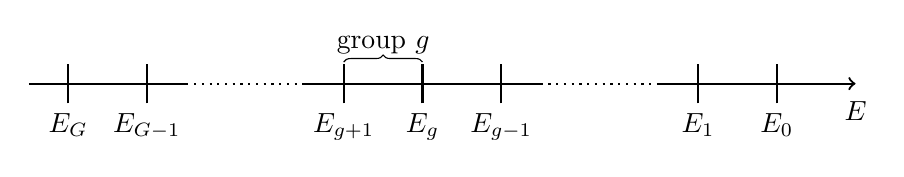
\begin{tikzpicture}
\draw[thick] (-5,0) -- (-3,0);
\draw[thick,dotted] (-3,0) -- (-1.5,0);
\draw[thick] (-1.5,0) -- (1.5,0);
\draw[thick,dotted] (1.5,0) -- (3,0);
\draw[thick,->] (3,0) -- (5.5,0);
\draw[thick] (-4.5,-0.25)--(-4.5,0.25);
\node [below] at (-4.5,-0.25) {$E_G$};
\draw[thick] (-3.5,-0.25)--(-3.5,0.25);
\node [below] at (-3.5,-0.25) {$E_{G-1}$};
\draw[thick] (-1,-0.25)--(-1,0.25);
\node [below] at (-1,-0.25) {$E_{g+1}$};
\draw[thick] (0,-0.25)--(0,0.25);
\node [below] at (0,-0.25) {$E_{g}$};
\node[above] at (-0.5, 0.25) {group $g$};
\draw[decorate,decoration={brace}](-1,0.275) -- (0,0.275);
\draw[thick] (1,-0.25)--(1,0.25);
\node [below] at (1,-0.25) {$E_{g-1}$};
\draw[thick] (3.5,-0.25)--(3.5,0.25);
\node [below] at (3.5,-0.25) {$E_1$};
\draw[thick] (4.5,-0.25)--(4.5,0.25);
\node [below] at (4.5,-0.25) {$E_0$};
\node [below] at (5.5,-0.1) {$E$};
\end{tikzpicture}
\caption{Discretized energy grid.}
\label{egrid}
\end{figure}

\FloatBarrier
Discretizing the NTE with respect to energy on this grid gives the $G$ multigroup
equations

\noindent\begin{minipage}{0.7\textwidth}
\begin{multline*}
\label{eq:mg_nte}
\bo \cdot \nabla \psi^g(\vecr,\bo) + \Sigma_t^g(\vecr) \psi^g(\vecr,\bo) =  \\
\sum_{g'=0}^{G-1}\int_{4\pi} \Sigma_s^{g'\rightarrow g}(\vecr,\bo'\cdot\bo)
\psi^{g'}(\vecr,\bo')d\bo' + Q^g(\vecr,\bo),
\end{multline*}
\end{minipage}
\hspace{-0.5cm}
\begin{minipage}{0.3\textwidth}
\begin{align}
\begin{split}
g &= 0,1,\ldots,G-1.
\end{split}
\end{align}
\end{minipage}
\vspace{0.1cm}

\noindent Here it is assumed that, within each energy group, the angular flux may be
approximated as the product of some known function of energy $f(E)$ and the group flux
$\psi^g(\vecr, \bo)$ as

\begin{equation}
\psi(\vecr,E,\bo) \approx f(E)\psi^g(\vecr,\bo), \quad E_{g+1} < E \leq E_{g}\:,
\end{equation}

\noindent where $f(E)$ is normalized such that $\int_{E_g+1}^{E_{g}}f(E)dE = 1$. With 
this, the multigroup cross sections and the group source are similarly defined
\cite{lm} as

\begin{align}
\Sigma_t^g(\vecr) &= \int_{E_{g+1}}^{E_{g}}\Sigma_t(\vecr,E)f(E)dE, \\
\Sigma_s^{g'\rightarrow g}(\vecr,\bo'\cdot\bo) &= \int_{E_{g+1}}^{E_{g}}\int_{E_{g'+1}}^{E_{g'}}
\Sigma_s(\vecr, E'\rightarrow E, \bo'\cdot\bo)f(E')dE'dE, \\
Q^g(\vecr,\bo) &= \int_{E_{g+1}}^{E_{g}}Q(\vecr,E,\bo)dE.
\end{align}

\paragraph{Spatial Discretization}\mbox{} \\

In the interest of completeness, we will briefly discuss the discretization of space.
The LDO equations are inherently three-dimensional \cite{ahrens}, so we will restrict
the discussion to three-dimensional space with point positions specified by Cartesian
coordinates. A general mesh cell is shown in Figure \ref{fig:spatial_mesh}.

\begin{figure}[!htb]
\centering
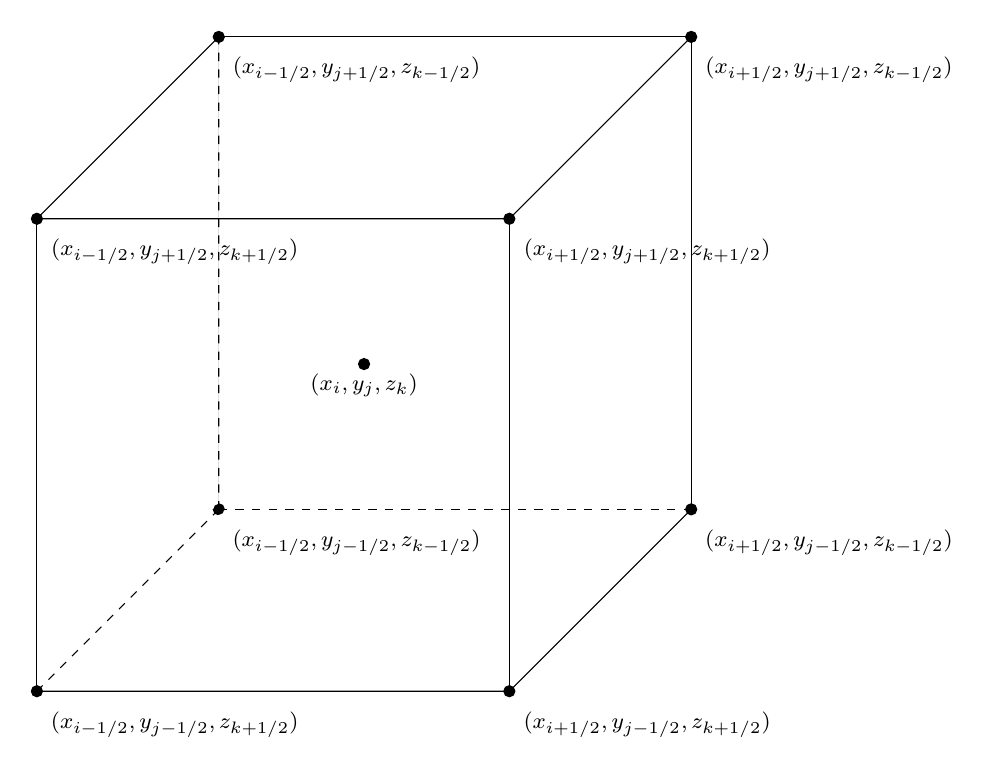
\begin{tikzpicture}
\filldraw (xyz cs:x=-3,y=-3,z=3) circle (2pt) node {} -- 
          (xyz cs:x=3,y=-3,z=3) circle (2pt) node {};
\node[fill,circle,inner sep=0pt, minimum size = 2pt,
      label={[shift={(1.75,-0.75)}]
      \footnotesize$(x_{i-1/2}, y_{j-1/2}, z_{k+1/2})$}] 
      at (xyz cs:x=-3,y=-3,z=3) {};
\node[fill,circle,inner sep=0pt, minimum size = 2pt,
      label={[shift={(1.75,-0.75)}]
      \footnotesize$(x_{i+1/2}, y_{j-1/2}, z_{k+1/2})$}] 
      at (xyz cs:x=3,y=-3,z=3) {};
\filldraw (xyz cs:x=-3,y=3,z=3) circle (2pt) node {} -- 
          (xyz cs:x=3,y=3,z=3) circle (2pt) node {};
\node[fill,circle,inner sep=0pt, minimum size = 2pt,
      label={[shift={(1.75,-0.75)}]
      \footnotesize$(x_{i-1/2}, y_{j+1/2}, z_{k+1/2})$}] 
      at (xyz cs:x=-3,y=3,z=3) {};
\node[fill,circle,inner sep=0pt, minimum size = 2pt,
      label={[shift={(1.75,-0.75)}]
      \footnotesize$(x_{i+1/2}, y_{j+1/2}, z_{k+1/2})$}] 
      at (xyz cs:x=3,y=3,z=3) {};
\filldraw (xyz cs:x=-3,y=3,z=3) -- 
          (xyz cs:x=-3,y=3,z=-3) circle (2pt) node[] {};
\node[fill,circle,inner sep=0pt, minimum size = 2pt,
      label={[shift={(1.75,-0.75)}]
      \footnotesize$(x_{i-1/2}, y_{j+1/2}, z_{k-1/2})$}] 
      at (xyz cs:x=-3,y=3,z=-3) {};
\filldraw (xyz cs:x=3,y=3,z=3)  -- 
          (xyz cs:x=3,y=3,z=-3) circle (2pt) node {};
\node[fill,circle,inner sep=0pt, minimum size = 2pt,
      label={[shift={(1.75,-0.75)}]
      \footnotesize$(x_{i+1/2}, y_{j+1/2}, z_{k-1/2})$}] 
      at (xyz cs:x=3,y=3,z=-3) {};
\filldraw (xyz cs:x=3,y=-3,z=3) -- 
          (xyz cs:x=3,y=-3,z=-3) circle (2pt) node {};
\node[fill,circle,inner sep=0pt, minimum size = 2pt,
      label={[shift={(1.75,-0.75)}]
      \footnotesize$(x_{i+1/2}, y_{j-1/2}, z_{k-1/2})$}]
      at (xyz cs:x=3,y=-3,z=-3) {};
\draw (xyz cs:x=-3,y=-3,z=3) -- (xyz cs:x=-3,y=3,z=3);
\draw (xyz cs:x=3,y=-3,z=3) -- (xyz cs:x=3,y=3,z=3);
\draw (xyz cs:x=-3,y=3,z=-3) -- (xyz cs:x=3,y=3,z=-3);
\draw (xyz cs:x=3,y=-3,z=-3) -- (xyz cs:x=3,y=3,z=-3);
\node[fill,circle,inner sep=0pt, minimum size = 2pt,
      label={[shift={(1.75,-0.75)}]
      \footnotesize$(x_{i-1/2}, y_{j-1/2}, z_{k-1/2})$}] 
      at (xyz cs:x=-3,y=-3,z=-3) {};
\filldraw[dashed] (xyz cs:x=-3,y=-3,z=-3) circle (2pt) node {} -- 
                  (xyz cs:x=-3,y=3,z=-3);
\draw[dashed] (xyz cs:x=-3,y=-3,z=-3) -- (xyz cs:x=3,y=-3,z=-3);
\draw[dashed] (xyz cs:x=-3,y=-3,z=-3) -- (xyz cs:x=-3,y=-3,z=3);
\filldraw (xyz cs: x=0,y=0,z=0) circle (2pt) node[below] 
          {\footnotesize$(x_i, y_j, z_k)$};
\end{tikzpicture}
\caption{General three-dimensional mesh cell \cite{exmm}.}
\label{fig:spatial_mesh}
\end{figure}

The mesh cell is centered at the $i^{th}$ position along the $x$-axis, the $j^{th}$
position along the $y$-axis, and the  $k^{th}$ position along the $z$-axis. Indexing
is such that there are $I$ mesh cells with $I+1$ grid points in the $x$-direction, $J$ mesh
cells with $J+1$ grid points in the $y$-direction, and $K$ mesh cells with $K+1$ grid points in 
the $z$-direction. It is assumed that all material 
properties are constant within a given cell. In order to eventually solve for the 
scalar flux in a given system, we are interested in solving for the angular flux at 
the center of each mesh cell, resulting in the $G\times I \times J \times K$
equations shown in Equation \ref{eq:mg_xyz_nte}.

\begin{minipage}{0.65\textwidth}
\begin{multline*}
\label{eq:mg_xyz_nte}
\bo\cdot\nabla\psi^g_{i,j,k}(\bo)+\Sigma_{t,i,j,k}^g\psi^g_{i,j,k}(\bo) =  \\
\sum_{g'=0}^{G-1}\int_{4\pi} \Sigma_{s,i,j,k}^{g'\rightarrow g}(\bo'\cdot\bo)
\psi^{g'}_{i,j,k}(\bo')d\bo' + Q^g_{i,j,k}(\bo),
\end{multline*}
\end{minipage}
\begin{minipage}{0.31\textwidth}
\begin{align}
\begin{split}
g &= 0,1,\ldots,G-1,\\
i &= 1,2,\ldots,I,\\
j &= 1,2,\ldots,J,\\
k &= 1,2,\ldots,K.
\end{split}
\end{align}
\end{minipage} \strut

\noindent To solve for these cell-centered flux 
quantities in practice, auxiliary equations are introduced. As these are specific to the 
spatial discretization employed in a given solution and do not differ between the classical
discrete ordinates equations and the LDO formulation, we refer the reader to Reference
\cite{denovo} for more detail on spatial differencing and solution methods.

\paragraph{Angular Discretization - Discrete Ordinates}\mbox{} \\
\label{sec:do}

The last part of phase space to discretize in the time-independent NTE is angle.
The discrete ordinates method is the most common angular discretization method
incorporated into general-purpose neutron transport codes \cite{lm}. It is a 
collocation method that requires the solution of the NTE to be exact at a 
distinct number of angles $\bo_n$:

\noindent\begin{minipage}{0.69\textwidth}
\begin{align*}
\bo_n&\cdot\nabla\psi^{g,n}_{i,j,k}+\Sigma_{t,i,j,k}^g\psi^{g,n}_{i,j,k} = \\
&\sum_{g'=0}^{G-1}\sum_{\ell=0}^P \Sigma_{s,\ell,i,j,k}^{g'\rightarrow g}
\bigg[\Ye{\ell 0}{n}\phi_{\ell 0}^{g'} + \sum_{m=1}^{\ell}
\bigg(\Ye{\ell m}{n}\phi_{\ell m}^{g'} \\
&\qquad\qquad\qquad\qquad\qquad\qquad
 + \Yo{\ell m}{n}\vartheta_{\ell m}^{g'}\bigg)\bigg]
 + Q^{g,n}_{i,j,k},
\end{align*}
\end{minipage}
\hspace{-0.55cm}
\begin{minipage}{0.31\textwidth}
\begin{align}
\begin{split}
g &= 0,1,\ldots,G-1,\\
i &= 1,2,\ldots,I,\\
j &= 1,2,\ldots,J,\\
k &= 1,2,\ldots,K,\\
n &= 1,2,\ldots,N.
\label{eq:do}
\end{split}
\end{align}
\end{minipage}
\vspace{0.1cm}

\noindent Here, $\psi^n \equiv \psi(\bo_n)$ and the angles are integrated by a
quadrature rule such that their corresponding weights $w_n$ sum to $4\pi$. Weights and
ordinates (``quadrature sets'') are chosen in such a way as to provide good 
approximations to angular integrals used to evaluate scalar flux \cite{lm,exmm}. The 
upper limit of summation for the scattering term spherical harmonic expansion, denoted
as $P$ in Equation \ref{eq:do}, is known as the ``\pn order''. The scattering cross section
coefficient values $\Sigma_{s,\ell,i,j,k}^{g'\rightarrow g}$ come from data libraries based on
experimental measurements.

The scattering source is expanded in terms of spherical harmonics:

\begin{equation}
\phi_{\ell,i,j,k}^{g}=\sum_{n=1}^N \Ye{\ell m}{n}w_n\psi^{g,n}_{i,j,k}\ \text{ and }\
\vartheta_{\ell,i,j,k}^{g} = \sum_{n=1}^N \Yo{\ell m}{n}w_n\psi^{g,n}_{i,j,k},
\label{sph_harm_exp}
\end{equation}

\noindent where $\phi$ and $\vartheta$ are
referred to as the ``flux moments''. 
Here, $\Ye{\ell m}{n}$ and $\Yo{\ell m}{n}$ are the ``even'' and ``odd'' 
real components of the spherical harmonic functions, defined as \cite{exmm}

\begin{equation}
\Ye{\ell m}{n} = (-1)^m\sqrt{(2-\delta_{m0})\frac{2\ell+1}{4\pi}
                       \frac{(\ell-m)!}{(\ell+m)!}}
                       P_{\ell m}(\cos\theta)\cos(m\varphi),
\label{eq:sph_e}
\end{equation}
\begin{equation}
\Yo{\ell m}{n} = (-1)^m\sqrt{(2-\delta_{m0})\frac{2\ell+1}{4\pi}
                       \frac{(\ell-m)!}{(\ell+m)!}}
                       P_{\ell m}(\cos\theta)\sin(m\varphi).
\label{eq:sph_o}
\end{equation}

\noindent In Equations \ref{eq:sph_e} and \ref{eq:sph_o}, $P_{\ell m}(\cos\theta)$ is 
the associated Legendre polynomial and $(\theta,\varphi)$ are the components of $\bo$ 
as shown in Figure \ref{fig:ang} and Equations \ref{eq:ang_disc} -- \ref{eq:ang_sum}. It is
assumed that the double differential scattering cross section depends only on the dot product of
the incoming and outgoing angles of the particle undergoing scattering.

To summarize Equations 
\ref{eq:do} -- \ref{eq:sph_o}, we note that the double differential scattering cross section is
expanded into the real components of the spherical harmonic functions, which can be represented
with Legendre polynomials; these are then multiplied with the angular flux moments expanded into
spherical harmonic functions.

\begin{figure}[!hbt]
\begin{minipage}{0.5\textwidth}
\begin{tikzpicture}
\coordinate (origin) at (0,0,0);
\coordinate (omega) at (2,4,7);
\coordinate (xaxis) at (0,0,9);
\coordinate (yaxis) at (3,0,0);
\coordinate (diag) at (2,5,0);
% axes
\draw[thick,->] (xyz cs:x=0) -- (xyz cs:x=3) node[right] {$x$};
\draw[thick,->] (xyz cs:y=0) -- (xyz cs:y=5) node[above] {$y$};
\draw[thick,->] (xyz cs:z=0) -- (xyz cs:z=8) node[below] {$z$};
% dashed box lines
\draw[dashed] (xyz cs:z=7,y=4) -- (xyz cs:z=7,y=0.25) node[left] {$\xi$};
\draw[dashed] (xyz cs:z=7,y=0) -- (xyz cs:z=7,x=2);
\draw[dashed] (xyz cs:z=7,x=2) -- (xyz cs:z=7,y=4,x=2);
\draw[dashed] (xyz cs:z=7,y=4,x=0) -- (xyz cs:z=7,y=4,x=2);

\draw[dashed] (xyz cs:x=2,z=0) -- (xyz cs:x=2,z=7);
\draw[dashed] (xyz cs:x=2,z=0,y=4) -- (xyz cs:x=2,z=0); 
\draw[] (xyz cs:x=2.3,y=-0.1,z=0) -- (xyz cs:x=2.3,y=-0.1,z=0) node[above] {$\mu$};
\draw[dashed] (xyz cs:x=2,z=0,y=4) -- (xyz cs:x=0,z=0,y=4) node[left] {$\eta$}; 
\draw[dashed] (xyz cs:x=0,z=0,y=4) -- (xyz cs:z=7,y=4);
\draw[dashed] (xyz cs:x=2,z=0,y=4) -- (xyz cs:z=7,y=4,x=2);

\draw[thick,->] (xyz cs:x=0,y=0,z=0) -- (xyz cs:x=2,z=7,y=4);
\draw[] (xyz cs:x=2,z=7,y=4) -- (xyz cs:x=2,z=7,y=4) node[above] {$\bo$};
\draw[dashed] (xyz cs:x=2,z=0,y=4) -- (xyz cs:x=0,z=0);
\draw[dashed] (xyz cs:z=7,y=0) -- (xyz cs:x=2,z=7,y=4);

\pic [draw,<-,angle radius=0.3cm,angle eccentricity=1.4,"$\theta$"]
     {angle = omega--origin--xaxis};
\pic [draw,->,angle radius=0.5cm,angle eccentricity=1.4,"$\varphi$"]
     {angle = yaxis--origin--diag};
\end{tikzpicture}
\caption{Angular coordinate system \cite{exmm}.}
\label{fig:ang}
\end{minipage}
\begin{minipage}{0.5\textwidth}
\begin{subequations}
\begin{align}
\label{eq:ang_disc}
&\xi = \cos\theta \\
&\mu = \sqrt{1-\xi^2}\cos\varphi \\
&\eta = \sqrt{1-\xi^2}\sin\varphi
\end{align}
\end{subequations}
\begin{equation}
\label{eq:ang_sum}
\mu^2 + \eta^2 + \xi^2 = 1
\end{equation}
\end{minipage}
\end{figure}

\FloatBarrier Commonly-used quadrature sets include level-symmetric, Gauss-
Legendre product, quadruple range (QR) product, and linear-discontinuous
finite element (LDFE). The various quadrature set types have different
properties with each being better for certain classes of problems. For
example, relatively coarse (sixteen angles per octant) QR product quadratures
are generally sufficient for generating variance reduction parameters for
neutron transport problems, but more finely resolved quadrature sets are
recommended for photon transport problems \cite{advantg}. Level-symmetric
quadrature sets are widely applied for general applications \cite{lm} but
tend to exhibit far more ray effects than QR product quadratures
\cite{advantg}. In the following subsection, we will discuss ray effects in
greater detail.

\subsubsection{Ray Effects}
\label{sec:ray}

Ray effects are unphysical computational anomalies in the scalar flux solution that 
arise from the discrete ordinates formulation. Because the NTE is only evaluated  
 at a finite number of discrete angles, the number of directions in 
which particles may stream is restricted. As a consequence of this, contributions to 
the scalar flux from uncollided particles are limited to those from the discrete 
angles along which particle sources are ``visible'' \cite{lathrop}. A demonstrative
example of ray effects is shown in Figure \ref{fig:ray}. The plot shows results from 
the PARTISN \cite{partisn} code using a triangular $P_n - T_n$ quadrature with
48 points and a
scattering ratio of $c = 0.25$ \cite{ahrens}. Although the point source
emits neutrons isotropically, the scalar flux calculated at a given radius out from 
the source sees contributions only from the discrete angles along which particles may
stream. That is, the flux at a given distance from the point source is actually equal 
in all directions and so the figure should appear to be a sphere, but the discrete
angles restrict streaming pathways to the rays shown in the image. 

\begin{figure}[!htb]
\centering
\includegraphics[width=0.5\textwidth]{img/ray-effects.png}
\caption{Isosurface plot of scalar flux from a point source \cite{ahrens}.}
\label{fig:ray}
\end{figure}

The severity of ray effects in a given simulation depends on the properties of
the  sources. The largest consequences tend to occur in scenarios with localized
sources and relatively minimal scattering. When using the discrete ordinates
approximation in a purely absorbing medium, regardless of the accuracy of the
angular flux calculations and the number of discrete angles used, it is always
possible to get far enough away from a localized source such that a poor value
of the scalar flux is obtained at that point \cite{lathrop}. In a scattering
medium with localized sources, angular flux values are incorrect because they
depend  on integrals that are poorly approximated by the quadrature formulation.
In contrast  to this, neutrons exiting scattering reactions are generally less
localized and  consequently tend to  mitigate ray effects. As we will see later
in the chapter, one key point of interest in using the LDO equations as part of
a hybrid method calculation is that the LDO equations mitigate ray effects when
higher-order quadrature sets are used  \cite{ahrens}.

\subsection{Hybrid Methods}

Hybrid methods aim to combine the previously described Monte Carlo
methods and deterministic methods in such a way as to perform calculations that result
in statistically meaningful results within a tractable period of computation time.
Generally, these hybrid methods are implemented such that the solution(s) from a 
deterministic code are used to inform a Monte Carlo code. When this is done well, the
Monte Carlo code converges more quickly than without the information from the
deterministic solution(s).

Specifically, an adjoint and/or forward flux solution generated by a deterministic 
transport solver is used to make a weight window map for a Monte Carlo run. As was
noted earlier, weight windows are most effective when specified well and when used in
conjunction with other variance reduction techniques. Because developing effective
weight window maps can be labor-intensive and require a user to have significant 
\textit{a priori} knowledge about the problem being solved, automated hybrid methods
have been developed to couple deterministic solutions to Monte Carlo transport
calculations.

\section{Previous Work}

Substantial effort has been placed into the development and automated execution of
hybrid methods. This section will discuss previous work in this field with a 
particular emphasis on the present state of hybrid methods as well as hybrid methods 
that incorporate neutron direction of travel.

Here we begin by describing the CADIS (consistent adjoint driven importance sampling)
and \fwc\ (forward-weighted consistent adjoint driven importance sampling) methods, 
which are the current state
of the art of Monte Carlo variance reduction parameter generation. These are 
introduced first because, as will be described in more detail later, this work 
employs solutions of the LDO equations in combination with the CADIS and \fwc\ 
methods via the ADVANTG software. Following this, we present a discussion of selected 
work in angle-informed hybrid methods, focusing on variants of CADIS and \fwc.

\subsection{CADIS and FW-CADIS}

\subsubsection{CADIS}
\label{sec:cadis}

The CADIS method was introduced by Wagner and Haghighat in 1997 to automate Monte 
Carlo variance reduction parameter generation \cite{cadis}. CADIS is based on the 
source biasing and weight window techniques described above, does not depend heavily 
on user experience, and was implemented as described in Reference \cite{cadis} in the 
MCNP \cite{mcnp} code. Most importantly, the CADIS method produces source biasing 
parameters and weight window target values such that particles are born with the target
weights. Since CADIS is used heavily in this work, it is pertinent to 
describe the theory behind the method.

The goal of most Monte Carlo neutron transport problems is to calculate some response
(scalar flux, dose, etc.) at some location in phase-space. This can be posed as 
solving the following integral equation:

\begin{equation}
R = \int_P \psi(P)\sigma_d(P)dP,
\label{eq:cadis_r1}
\end{equation}

\noindent where $R$ is the response of interest, $\psi$ is the neutron angular flux,
and $\sigma_d$ is some objective function in the phase-space $(\vecr, E, \bo) \in P$.
We now introduce the adjoint identity

\begin{equation} 
\langle \psi^{\dagger}, H\psi\rangle=\langle\psi , H^{\dagger}\psi^{\dagger}\rangle
\label{eq:adj}
\end{equation}

\noindent where $H$ is the transport operator and the dagger superscript indicates an 
adjoint quantity. Using Equation \ref{eq:adj} and some algebraic manipulations, it 
can be shown that

\begin{equation}
R = \int_P \psi^{\dagger}(P)q(P)dP,
\label{eq:cadis_r2}
\end{equation}

\noindent where $\psi^{\dagger}$ and $q$ are the adjoint neutron angular flux function
and the particle source density, respectively. For a given problem with a vacuum 
boundary condition, Equations \ref{eq:cadis_r1} and \ref{eq:cadis_r2} are equivalent 
expressions for $R$. The adjoint neutron angular flux function $\psi^{\dagger}$ has 
physical meaning as the expected contribution to the response $R$ from a particle in 
phase-space $P$. In other words, the adjoint flux function is significant because it 
represents the importance of those source particles to the response of interest.

To calculate the response with the Monte Carlo method, the independent variables are
sampled from the probability density function (PDF) $q(P)$. However, this may not be
the best PDF from which to sample, so an alternative PDF $\qhat(P)$ can be introduced
into the integral:

\begin{equation}
R = \int_P \left[\frac{\psi^{\dagger}(P)q(P)}{\qhat(P)}\right]\qhat(P)dP,
\end{equation}

\noindent where $\qhat(P) \geq 0$ and the integral of $\qhat(P)$ over $P$ is 
normalized to unity. Then, the alternative PDF $\qhat(P)$ that will minimize the 
variance of the response is given by

\begin{equation}
\qhat(P) = \frac{\psi^{\dagger}(P)q(P)}{\int_P\psi^{\dagger}(P)q(P)dP}.
\label{eq:qhat}
\end{equation}

\noindent Looking at Equation \ref{eq:qhat}, we see that the numerator is the 
response from phase-space $P$ and the denominator is the total response $R$. Thus, 
this definition of $\qhat(P)$ is a measure of the contribution from phase-space $P$ 
to the response. It is useful to bias the sampling of source particles by this ratio 
of their contribution to the detector response.

Because the source variables are sampled from this new biased PDF, the statistical
weight of the source particles must be corrected such that

\begin{equation}
w(P)\qhat(P) = w_0q(P),
\label{eq:cadis_w1}
\end{equation}

\noindent where $w_0$ is the unbiased particle starting weight and is set equal to 1.
Substituting Equation \ref{eq:qhat} into Equation \ref{eq:cadis_w1} and solving for 
$w(P)$ gives the following expression for the statistical weight of the particles:

\begin{equation}
w(P) = \frac{\int_P\psi^{\dagger}(P)q(P)dP}{\psi^{\dagger}(P)}
= \frac{R}{\psi^{\dagger}(P)}.
\label{eq:cadis_w2}
\end{equation}

\noindent Equation \ref{eq:cadis_w2} demonstrates an inverse relationship between 
this adjoint (importance) function and the statistical particle weight. 

Now, let us consider the
transport process in this context. The integral transport equation for particle
density in the phase-space $P$ is given by

\begin{equation}
\psi(P) = \int K(P'\rightarrow P)\psi(P')dP' + q(P)
\label{eq:cadis_nte1}
\end{equation}

\noindent where $K(P'\rightarrow P)$ is the expected number of particles entering $dP$
about $P$ from an event in $P'$. Given the preceding discussion, we would like to 
transform Equation \ref{eq:cadis_nte1} to be in terms of the biased source 
distribution $\qhat(P)$. Defining

\begin{equation}
\psihat(P) = \frac{\psi(P)\psi^{\dagger}(P)}{\int \psi^{\dagger}(P)q(P)dP},
\end{equation}

\noindent we can write Equation \ref{eq:cadis_nte1} in terms of $\qhat(P)$ as

\begin{equation}
\psihat(P) = \frac{\psi^{\dagger}(P)}{\int \psi^{\dagger}(P)q(P)dP}
\int K(P'\rightarrow P)\psi(P')dP' + \qhat(P).
\label{eq:cadis_nte2}
\end{equation}

\noindent Equation \ref{eq:cadis_nte2} can also be written as

\begin{equation}
\psihat(P) = \int K(P'\rightarrow P)\psihat(P')
\left[\frac{\psi^{\dagger}(P)}{\psi^{\dagger}(P')}\right]dP' + \qhat(P)\:,
\end{equation}

\noindent which allows us to define

\begin{equation}
\khat(P' \rightarrow P) = K(P'\rightarrow P)
\left[\frac{\psi^{\dagger}(P)}{\psi^{\dagger}(P')}\right]
\end{equation}

\noindent and finally write

\begin{equation}
\psihat(P) = \int\khat(P' \rightarrow P)\psihat(P')dP' +\qhat(P).
\end{equation}

Because $K(P'\rightarrow P)$ is unknown, we simulate neutron transport in the usual
unbiased way and change the number of particles emerging in $P$ from an event in
$P'$ by the ratio of importances $\psi^{\dagger}(P)/\psi^{\dagger}(P')$. When this
ratio is above one, splitting occurs, and rouletting occurs when the ratio is less 
than one. The statistical weights of the particles resulting from splitting and/or
rouletting are then corrected such that

\begin{equation}
w(P)K(P' \rightarrow P)\left[\frac{\psi^{\dagger}(P)}{\psi^{\dagger}(P')}\right] = 
w(P')K(P' \rightarrow P)
\end{equation}

\noindent or

\begin{equation}
w(P) = w(P')\left[\frac{\psi^{\dagger}(P)}{\psi^{\dagger}(P')}\right].
\label{eq:cadis_w3}
\end{equation}

\noindent With this, reduced variance can be achieved when all source and transport
sampling is proportional to its importance. The source particles' energy and position
are sampled from the biased source distribution

\begin{equation}
\qhat(\vecr,E) = 
\frac{\phi^{\dagger}(\vecr,E)q(\vecr,E)}
{\int_V\int_E\phi^{\dagger}(\vecr,E)q(\vecr,E) dE\ d\vecr} 
= \frac{\phi^{\dagger}(\vecr,E)q(\vecr,E)}{R}.
\label{eq:cadis_sb}
\end{equation}

\noindent Here, the physical meaning of the numerator is the detector response from
space-energy element $(d\vecr,dE)$ and the denominator is the total detector response
$R$. As in the preceding derivation, this ratio is a measure of the particles' 
relative contribution to the detector response.

To bias particles undergoing the transport process, the weight window technique is 
applied. Weight window lower bounds $w_{\ell}$ must be calculated such that the
statistical weights defined in Equation \ref{eq:cadis_w2} fall at the center of the
weight window intervals. The width of a given interval is denoted by 
$c_u = w_u/w_{\ell}$, the ratio of upper and lower weight window values. The
weight window lower bounds are then given by

\begin{equation}
w_{\ell}(\vecr,E) = \frac{w}{\left(\frac{c_u +1}{2}\right)} 
= \frac{R}{\phi^{\dagger}(\vecr,E)}\frac{1}{\left(\frac{c_u +1}{2}\right)}.
\label{eq:cadis_tb}
\end{equation}

\noindent Using this definition, the weight window technique then performs particle
splitting and/or rouletting consistent with the statistical weight given in Equation
\ref{eq:cadis_w3}.

The key result of the foregoing discussion is that the statistical weights of the
source particles are within the bounds of the weight windows. In other words, the
source-biasing parameters and the weight window target values are consistent. This
circumvents the potential of particles being immediately split or rouletted upon birth
and avoids the resultant degradation in computational efficiency. We refer the reader
to Reference \cite{cadis} for a complete discussion of results and analysis of the initial
implementation of the CADIS method.

Note that Equations \ref{eq:cadis_sb} and \ref{eq:cadis_tb} use the scalar adjoint 
flux rather than the angular flux. This is consistent with the
original implementation of the CADIS method in MCNP as well as the implementation of
the method in ADVANTG; the scalar adjoint neutron flux function is used in both tools
\cite{cadis, advantg}. Historically, this was done to reduce the memory required for
the deterministic calculation as well as the weight window map. Additionally, the 
angular adjoint flux resulting from an \sn calculation was not considered to be 
sufficiently accurate due to the limited number of discrete angles used for the 
calculation. Further, people have
generally not developed weight windows that are a function of angle.

The CADIS method is very effective for automated optimization of localized detectors
but falls short of efficiently optimizing distributed responses. FW-CADIS, discussed 
in the next section, was developed to address this issue.

\subsubsection{FW-CADIS}
\label{sec:fwcadis}

FW-CADIS, introduced
by Wagner, Blakeman, and Peplow in 2009, is a variation on the CADIS method to 
increase the efficiency of Monte Carlo calculations of distributions and responses at 
multiple localized detectors \cite{fwcadis}.

For this global variance reduction method, a response with uniformly-low statistical 
uncertainty across all phase-space is desired. One way to target this for a given 
Monte Carlo simulation is to uniformly distribute the particles throughout the system.
Though this is not a physical response, it is a proxy for the goal of obtaining 
uniform uncertainty. It also indicates the possibility of developing an adjoint 
importance function that represents the importance of particles to achieving the goal
of uniform particle distribution.

With this new problem formulation, the problem of calculating particle density is cast
into the response formulation:

\begin{equation}
R = \int_{4\pi}\int_{V}\int_{E}\psi(\vecr,E,\bo)f(\vecr,E,\bo)dE\ dV\ d\bo,
\end{equation}

\noindent where $f(\vecr,E,\bo)$ is some function that converts angular neutron flux 
to Monte Carlo particle density. Recall that the angular neutron flux can be defined 
as the product of the physical particle density $n$ and velocity $v$:

\begin{equation}
\psi(\vecr,E,\bo) = n(\vecr,E,\bo)v(\vecr,E,\bo)
\label{eq:psi}
\end{equation}

\noindent and the physical particle density is related to the Monte Carlo particle 
density $m$ and the average particle weight $\bar{w}$ by

\begin{equation}
n(\vecr,E,\bo) = \bar{w}(\vecr,E,\bo)m(\vecr,E,\bo).
\label{eq:dens}
\end{equation}

\noindent Using Equations \ref{eq:psi} and \ref{eq:dens}, the Monte Carlo particle 
density can be estimated by

\begin{equation}
m(\vecr,E,\bo) = \frac{n(\vecr,E,\bo)}{\bar{w}(\vecr,E,\bo)} 
= \frac{\psi(\vecr,E,\bo)}{\bar{w}(\vecr,E,\bo)v(\vecr,E,\bo)}
\end{equation}

\noindent and the total Monte Carlo density can be estimated by

\begin{equation}
R = \int_{4\pi}\int_{V}\int_{E}\psi(\vecr,E,\bo)
\left[\frac{1}{\bar{w}(\vecr,E,\bo)v(\vecr,E,\bo)}\right]dE\ dV\ d\bo.
\label{eq:fwcadis_r}
\end{equation}

If the average particle weight is set proportional to the physical particle density,
then the Monte Carlo particle density should be approximately uniform in phase-space.
Substituting Equation \ref{eq:psi} into Equation \ref{eq:fwcadis_r} gives %eq 14

\begin{equation}
R = \int_{4\pi}\int_{V}\int_{E}\psi(\vecr,E,\bo)
\left[\frac{1}{\psi(\vecr,E,\bo)}\right]dE\ dV\ d\bo.
\end{equation}

\noindent By then defining the adjoint source as the bracketed term in the above
equation,

\begin{equation}
q^{\dagger}(\vecr,E,\bo) = \frac{1}{\psi(\vecr,E,\bo)},
\end{equation}

\noindent we can calculate an adjoint importance function that represents the
importance of particles to achieving the desired objective of uniformly distributed
Monte Carlo particles. This should, in turn, correspond to approximately uniform
statistical uncertainties. The method physically corresponds to weighting the adjoint
source with the inverse of the forward flux; the adjoint source will be high where the
forward flux is low and the adjoint source will be low where the forward flux is high.
With this method, after the adjoint has been determined, the standard CADIS procedures
are used to calculate consistent source biasing parameters and weight windows.

When considering implementation and use, it should be noted that, while the original
CADIS method requires only one deterministic calculation, the \fwc\ method requires
two (one forward and one adjoint) deterministic calculations. Additionally, like the
original CADIS method, \fwc\ is general and could be applied to all independent
variables of a problem, but the implementation has been limited to space and energy. 

\subsection{Directional CADIS}

Noting the marked performance of the CADIS and \fwc\ methods, their limited 
implementation in only space and energy, and the importance of particle direction, 
Peplow introduced directional CADIS in 2012 \cite{peplow}. Two versions of directional
CADIS were explored: one method that biases the source in space and energy while
preserving the original angular distribution of the particles, and one method that
biases the source in space, energy, and angle. Both new methods were tested against
standard CADIS for seven example problems, with the Monte Carlo FOM compared among the
methods for each problem.

Peplow notes that in many applications involving directionally dependent source 
distributions, the directional dependence is azimuthally symmetric about a given
reference direction $\mathbf{\hat{d}}$. With this, the angular distribution of the 
particles $q_i(\bo)$ can be expressed as the product of the uniform azimuthal 
distribution and a polar distribution about reference $\mathbf{\hat{d}}_i$. The 
angular particle distribution may then be written as 
$\frac{1}{2\pi}q_i(\bo\cdot\mathbf{\hat{d}}_i)$. Peplow also notes that the
geometric size of these directional sources tends to be small enough to allow each
source distribution to be expressed as the product of two separable distributions:
$q_i(\vecr,E,\bo) \approx q_i(\vecr, E)q_i(\bo)$.

The implementation of directional CADIS explored in this work was intended to
appropriately incorporate the importance of a particle traveling in a given direction
while also serving as a relatively simple modification of the standard CADIS method
that is less involved than a full treatment of space, energy, and angle. It starts 
with the approximation that the angular component of the adjoint flux 
$\psi^{\dagger}(\vecr,E,\bo)$ is separable and symmetric about the average adjoint
current direction $\hat{\mathbf{n}}(\vecr,E)$ such that

\begin{equation}
\psi^{\dagger}(\vecr,E,\bo) \approx
\phi^{\dagger}(\vecr,E)\frac{1}{2\pi}f(\bo\cdot\hat{\mathbf{n}}).
\end{equation}

\noindent From this, it is proposed that weight window targets can be developed that
are inversely proportional to the approximation of the adjoint angular flux:

\begin{equation}
\bar{w}(\vecr,E,\bo) = 
\frac{2\pi k}{\phi^{\dagger}(\vecr,E)f(\bo\cdot\hat{\mathbf{n}})}
\end{equation}

\noindent where $k$ is a constant of proportionality that is adjusted to make the
importance map consistent with the biased source(s). The implementation of the
following methods uses standard CADIS routines to compute the response per unit 
source $R$, the weight window target values $\bar{w}(\vecr,E)$, and the biased source 
$\hat{q}(\vecr,E)$ using only the adjoint scalar flux. The quantities are then
modified to include directional information.

\subsubsection{Without Directional Source Biasing}

Peplow asserts that the biased source $\hat{q}(\vecr,E,\bo)$ should be proportional
to both the true particle source distribution and the space-energy component of the
scalar adjoint flux:

\begin{equation}
\hat{q}(\vecr,E,\bo) = \frac{1}{R}
\left[q(\vecr,E)\frac{1}{2\pi}q(\bo\cdot\mathbf{\hat{d}})\right]
\phi^{\dagger}(\vecr,E),
\end{equation}

\noindent where the constant of proportionality $R$ is determined by forcing
$\hat{q}(\vecr,E,\bo)$ to be a PDF. Since the scalar adjoint flux is used here, the
directional distribution of the biased source is identical to that of the true source.
Detailed in Reference \cite{peplow}, the constant of proportionality $R$ is found to be equal to
the response per unit source from the traditional space-energy CADIS treatment. Thus,
the biased source can be expressed as

\begin{equation}
\hat{q}(\vecr,E,\bo) = \hat{q}(\vecr,E)\frac{1}{2\pi}q(\bo\cdot\mathbf{\hat{d}}). 
\end{equation}

The birth weight of a particle sampled from this distribution is independent of
direction and the proportionality constant $k$ for the target weight windows should be
chosen such that the weight window targets match the birth weight of the source
particles. This cannot be done generally because the particle birth weight is
independent of direction, but it can be done for a single point in phase space
$(\vecr_0,E_0,\bo_0)$ of the source such that

\begin{equation}
k = \frac{R}{2\pi}f\left(\bo_0\cdot\hat{\mathbf{n}}(\vecr_0,E_0)\right),
\end{equation}

\noindent where the average adjoint current direction $\hat{\mathbf{n}}(\vecr_0,E_0)$
is evaluated at the source location and energy and

\begin{equation}
\bar{w}(\vecr,E,\bo) = \bar{w}(\vecr,E)
\frac{f\left(\bo_0\cdot\hat{\mathbf{n}}(\vecr_0,E_0)\right)}
{f(\bo\cdot\hat{\mathbf{n}})}.
\end{equation}

\noindent Because the biased source and the weight window targets will match only at
the specified direction of interest $\bo_0$ at one specific position and energy, the
point $(\vecr_0,E_0,\bo_0)$ should be chosen carefully to represent the source
accurately and to minimize rouletting and/or splitting of particles just after birth.

It should be noted that this approach is exact for cases where no directional biasing
could be applied, e.g.\ monodirectional beam sources. Although the above discussion
considers only one particle source, this directional CADIS method may be extended to
multiple sources, as explained in detail in Reference \cite{peplow}.

\subsubsection{With Directional Source Biasing}

In this method, it is asserted that the biased source should be proportional
to both the true particle source distribution and the approximation of the angular
adjoint flux:

\begin{equation}
\hat{q}(\vecr,E,\bo) = \frac{1}{cR}
\left[q(\vecr,E)\frac{1}{2\pi}q(\bo\cdot\mathbf{\hat{d}}_i)\right]
\left[\phi^{\dagger}(\vecr,E)\frac{1}{2\pi}f(\bo\cdot\hat{\mathbf{n}}_0)\right],
\end{equation}

\noindent where the constant $cR$ is used to make $\hat{q}$ a PDF. Because the vector
$\hat{\mathbf{n}}_0$ is fixed over the source, the biased source is separable into
$\hat{q}(\vecr,E,\bo)=\hat{q}(\vecr,E)\hat{q}(\bo)$ where $\hat{q}(\bo)$ can be
further separated into the product of its azimuthal and polar distributions:

\begin{equation}
\hat{q}(\vecr,E,\bo) = 
\left[\frac{1}{R}q(\vecr,E)\phi^{\dagger}(\vecr,E)\right]
\left[\frac{1}{c}\frac{1}{4\pi^2}q(\bo\cdot\mathbf{\hat{d}})
f(\bo\cdot\hat{n}_0)\right].
\end{equation}

Both distributions $\hat{q}(\vecr,E)$ and $\hat{q}(\bo)$ are independent and each 
should be a PDF. For the space-energy distribution, the standard definition of $R$
still applies. For the angular distribution, the constant $c$ is found to be

\begin{equation}
c = \int\frac{1}{4\pi^2}q(\bo\cdot\hat{\mathbf{d}})f(\bo\cdot\hat{\mathbf{n}}_0)d\bo,
\end{equation}

\noindent which may be evaluated using numerical integration. It should be noted that
if either the original source directional distribution $q(\bo)$ or the adjoint
angular flux distribution at the source is isotropic, then $c$ reduces to a value of
$\frac{1}{4\pi}$.

Source particles sampled from the biased distribution are born with a starting weight
of

\begin{equation}
\bar{w}(\vecr,E,\bo) =
\frac{R}{\phi^{\dagger}(\vecr,E)}\frac{2\pi c}{f(\bo\cdot\hat{\mathbf{n}}_0)} = 
\bar{w}(\vecr,E)\frac{2\pi c}{f(\bo\cdot\hat{\mathbf{n}}_0)}\:,
\end{equation}

\noindent where the constant $k$ has been found to be equal to $cR$. As with the 
previously described method, the user selects one point $(\vecr_0,E_0,\bo_0)$ that is
representative of the entire source, where the biased source will match the target
weight windows. This method can also be extended to incorporate multiple sources.

\subsubsection{Results}

Sample problems of applications of interest were examined and compared between 
standard CADIS and directional CADIS. For most of these problems, directional CADIS 
outperformed standard CADIS, increasing the Monte Carlo FOM by a factor of around 2. Notable
cases in which directional CADIS performed more poorly than standard CADIS are a
neutron porosity tool problem and a gamma-ray litho-density tool problem with the
detector far away from the source. It should also be noted that, for a spherical boat
test problem with a source far away from the boat, both standard CADIS and directional
CADIS performed more poorly than an analog Monte Carlo calculation. For full details on the
test results, see Reference \cite{peplow}. In the conclusions of the report, Peplow 
notes that ``it is difficult to know \textit{a priori} which problems would benefit 
from the space/energy/angular treatments presented in this work more than from just 
using the standard space/energy CADIS.''

\subsection{CADIS-$\Omega$}

One of the most recent developments in the area of angle-informed hybrid methods is
\co, introduced by Munk et al.\ in 2016 \cite{cadisom}. This method calculates an
alternate form of the adjoint scalar flux quantity that is then used in the CADIS and
\fwc\ methods for generation of variance reduction parameters for local and global
response functions, respectively.

The alternative form of the adjoint scalar flux used in \co\ is defined as

\begin{equation}
\phi^{\dagger}_{\Omega}(\vecr,E) = 
\frac{\int_{4\pi} \psi(\vecr ,E,\bo)\psi^{\dagger}(\vecr,E,\bo)d\bo}
{\int_{4\pi}\psi(\vecr,E,\bo)d\bo}.
\end{equation}

\noindent Here, the product $\psi(\vecr ,E,\bo)\psi^{\dagger}(\vecr,E,\bo)$ is known
as the ``contributon flux''; contributons can be conceptualized as pseudo-particles
that carry ``response'' from a particle source to a detector. The contributon flux
incorporates information from both the forward particle flux as well as the adjoint
particle flux. It signifies the importance of a particle born from a forward source
moving towards an adjoint source. That is, when the contributon flux is used to 
generate an importance map, high importance will be assigned to particles that are
generated at the forward source and are likely to generate a response in the detector
(the adjoint source).

The \co\ method was implemented in the ADVANTG framework, with numerical experiments
performed testing variance reduction for problems run in MCNP5. Several
characterization problems with spatially-induced anisotropies were tested to
evaluate the new method when used with CADIS and \fwc. Here we will summarize the
problems tested and the results; a full discussion can be found in Reference 
\cite{munk}. Munk identified three categories of processes that affect particle flux 
anisotropy: strongly directional particle sources, strong differences between material
properties, and algorithmic limitations that result in ray effects.

Having grouped these processes, Munk tested a set of characterization problems, each
of which have different combinations of the above anisotropy-inducing mechanisms. Munk
also developed a set of metrics by which the anisotropy of the flux may be quantified
over the various problems. Similar to the conclusions drawn by Peplow, Munk found 
that it was difficult to predict for which problems \co\ should outperform CADIS. When
considering a parametric study of deterministic variables likely to affect angular 
flux (varying quadrature set order and \pn order) in a characteristic problem
composed of a steel beam embedded in concrete, \co\ achieved higher FOM values than 
standard CADIS for all quadrature and \pn orders at high energies. Similarly, for a
simple labyrinth geometry of an air maze through a concrete block, \co\ achieved lower
relative errors than did standard CADIS in the epithermal and fast neutron energy
groups.

\subsection{Other Notable Work}

Here we will briefly summarize other notable works in the area of angle-informed 
hybrid methods. We first introduce AVATAR, then discuss two following methods that
built off of the work.

\subsubsection{AVATAR}

AVATAR (Automatic Variance And Time of Analysis Reduction) was developed at Los Alamos
National Laboratory by Van Riper et al.\ in the 1990s to eliminate the need for
user-generated weight windows \cite{avatar}. The package may be thought of as a
predecessor to the various CADIS methods, as it constructs three-dimensional energy-
and angle-dependent weight windows for an MCNP run from an adjoint calculation using
the THREEDANT \cite{threedant} deterministic code.

The scalar adjoint fluxes resulting from THREEDANT are inverted by AVATAR to get the
lower weight window boundary in each mesh element of the problem. The weight windows
are then normalized such that source particles are born with weights inside of the
weight window. If angle-dependent weight windows are desired, the angular adjoint flux
is approximated using information theory \cite{avatar}; the full angular adjoint flux
was deemed to require an inordinate amount of storage at the time of development.

AVATAR's weight window mesh is independent of the Monte Carlo cells, so weight 
windows are applied at absolute particle positions rather than when particles pass
between weight window meshes. To protect against significant variance increases in
particle weight (and tally) due to large sampling distance, weight windows are applied
at a minimum of once per mean free path traveled by a particle.

AVATAR was tested on a model of a three-detector oil well logging tool consisting of
a gamma-ray source and three gadolinium detectors. The system was intended to
represent deep-penetration problems, as a small fraction of the gamma rays emitted
from the source actually reach the detectors. The detector nearest the gamma-ray
source has a collimator attached, adding an angular dependence to the tool modeled. 

Results from AVATAR were compared against MCNP's weight window generator (WWG). For
the three-detector problem described above, AVATAR's angle-dependent weight windows
delivered the highest FOM for the detector nearest the source as well as the 
``middle'' detector. The MCNP WWG delivered the highest FOM for
the detector furthest from the source, but it should be noted that the MCNP geometry
was hand-tuned for the WWG cases. When considering only a single detector, the
AVATAR angle-dependent weight windows outperformed the WWG for a detector near the
source as well as far from the source.

\subsubsection{Cooper and Larsen's Weight Windows}

Cooper and Larsen developed a method similar to FW-CADIS that uses weight windows to
distribute Monte Carlo particles uniformly throughout the system for the purpose of
efficiently solving global particle transport problems \cite{clww}. Rather than using
an adjoint deterministic solution for generation of weight windows, a forward solution
is used. The method presented employs solution of the forward quasi-diffusion 
equation, a modified diffusion equation that contains multiplicative correction terms
known as ``Eddington factors''.

The authors argue that a forward solution is more appropriate than an adjoint solution
in the context of automated weight window generation for Monte Carlo variance
reduction. This is supported by showing that if the center of the weight window in
each cell is chosen to be proportional to the density of the physical particles in the
cell, then the density of Monte Carlo particles throughout the system will be
approximately constant.

Cooper and Larsen construct ``isotropic'' weight windows as well as angle-dependent
weight windows, following the AVATAR method to formulate the latter. The authors note
that a uniform particle distribution in angle is not always optimal with respect to
computational efficiency, especially when considering problems with significant
streaming. It is the case that the angle-dependent weight windows developed in this 
work actually have the potential to reduce the FOM due to excessive Monte Carlo 
particle splitting in nonstreaming regions. To mitigate this by decreasing the amount 
of splitting incurred, the weight window experienced by particles traveling in 
directions opposite to the preferred direction is raised. This preserves the scalar 
flux, but not the current \cite{clww}.

Results are presented for two two-dimensional problems. In both problems, weight
windows were updated twice -- once after one-third of the histories had completed and
again after two-thirds of the particle histories had finished. The weight window
parameters were chosen to ensure a stable quasi-diffusion solution. The two problems
were chosen to rigorously test the global Monte Carlo method; the problems are
optically thick with scattering ratios sufficiently low such that the scalar flux
decreases by several orders of magnitude far away from the particle source. To 
observe the performance of the method on problems with significant angular effects,
the first problem includes a duct and the second problem includes a barrier.

For the problem including a duct, the Monte Carlo FOM values calculated in the 
individual spatial cells are vastly improved by the use of both weight window types
developed in this work. In particular, the solution estimates for the scalar flux are
very noisy far from the solution when only survival biasing is used. Additionally, the
angle-dependent weight window generates a slightly higher FOM in the duct region than
the isotropic weight window. Similarly, for the problem including a barrier, the use
of either type of weight window developed here results in a drastically more uniform
particle distribution. Again, the angular weight window outperformed the isotropic
weight window. Thus, from this work, we observe that incorporating angular
information into weight window generation can significantly improve Monte Carlo FOM
for problems with strong geometric anisotropies.

\subsubsection{LIFT}

LIFT, the local importance function transform, was introduced by Turner and Larsen in
1997 \cite{lift1, lift2} as a new automatic Monte Carlo variance reduction method that
closely approximates a zero-variance method through the use of biasing parameters. The
LIFT method is partially based on the exponential transform, which adjusts the 
distance to collision such that particles traveling toward the region of interest 
undergo fewer collisions than particles traveling away from the region of interest.
Particle weights are adjusted accordingly to keep the simulation unbiased. On top of
the conventional exponential transform, the LIFT method adds in energy and angular
biasing in each cell of the system.

LIFT uses scalar flux information from a deterministic adjoint solution to bias the
source distribution, distance to collision, scattering angle, and energy. The adjoint 
scalar flux is also used to formulate weight windows. In the implementation 
presented, the weight windows are not angle-dependent. The authors note that, in the 
LIFT implementation, the angle-dependent weight windows require the use of an 
analytic expression for the angular flux at every boundary and collision site and 
that this extra computational effort does not generally yield increased efficiency 
for the Monte Carlo calculation that then employs the angle-dependent weight windows.

The LIFT strategy can be summarized in two steps. First, an analytic function is
derived that is piecewise continuous in space and angle and approximates the adjoint
solution within each energy group and spatial cell of the Monte Carlo system. Then,
this approximate representation of the adjoint solution is used to transform the
original forward problem into a new problem that can be solved by a Monte Carlo 
simulation with reduced variance. Increased accuracy in the approximation of the
adjoint solution results in greater reduction of the variance, approaching zero
variance in the solution when using an exact representation. The authors note that 
this limit is unachievable and that the algebraic cost of obtaining and using more
accurate adjoint solutions must be balanced against the desired FOM. 

The authors compare LIFT against AVATAR, considered to be one of the most efficient
automated variance reduction techniques used in a major production code at the time of
publication. The overall result stated in Reference \cite{lift1} is that LIFT 
outperforms 
AVATAR in most problems. The reasons given for this are that LIFT particles have 
significantly shorter histories than AVATAR particles and that LIFT particles have
smaller weight fluctuations than AVATAR particles and thus require less splitting and 
Russian roulette. It is noted, however, that the two methods perform comparably for
problems where biasing is difficult (AVATAR does not use any biasing techniques other
than survival biasing, which LIFT also employs in addition to its other biasing).

It is seen that the LIFT method loses its advantage over survival biasing as the 
scattering ratio of a given problem approaches unity. While FOM values from LIFT
increase, the acceleration of the method compared to survival biasing becomes 
negligible \cite{lift1}. In Reference \cite{lift2}, numerical results and comparisons 
against
AVATAR are presented. We will briefly summarize the results and conclusions here,
focusing on results from the most complex scenario tested, as the work presented in 
this dissertation is concerned with three-dimensional multigroup problems.

Cooper and Larsen tested the LIFT method in combination with results from various
types of deterministic solutions as well as in combination with weight windows
generated from AVATAR. The most complex scenario tested was multigroup in energy 
and featured a concrete cube with a duct running through it. The duct was also
concrete but with a lower density than the bulk material; it had the source at one end,
the detector at the other end, and three bends along its path. In general, it was
found that incorporating angular information into the AVATAR and LIFT solutions 
improved the FOM for the Monte Carlo calculation when using either code \cite{lift2}.
Taking this result into consideration as well as other conclusions drawn in work 
discussed earlier in this chapter, we move forward onto discussing the LDO equations,
which will be developed and then used to incorporate angular information into Monte
Carlo variance reduction parameter generation.

\section{The Lagrange Discrete Ordinates (LDO) Equations}
\label{sec:ldo}

The Lagrange Discrete Ordinates (LDO) equations, shown in Equation \ref{eq:ldo}, are
formally the same as the classical discrete ordinates equations. The LDO equations
differ from the discrete ordinates equations in how the scattering source is 
calculated and in the representation of the angular flux. In this section, we give a
mathematical background for and a derivation of the LDO equations.

\subsection{Mathematical Background}
\label{sec:ldo_math}

Prior to deriving the LDO equations, it is useful to summarize relevant material from
approximation theory for functions defined on $\maths$, the unit sphere in 
$\mathbb{R}^3$. We start by denoting the space of square integrable functions on
$\maths$ as $L^2(\maths)$, where an orthonormal basis for $L^2(\maths)$ is given by 
the spherical harmonic functions

\begin{equation}
Y_{\ell}^m(\theta,\varphi) = (-1)^{\ell}
\sqrt{\frac{2\ell+1}{4\pi}\frac{(\ell-m)!}{(\ell+m)!}}
P_{\ell}^m(\cos\theta)e^{im\varphi}.
\end{equation}

\noindent Here, $\ell\geq 0$, $|m| \leq \ell$, $P_{\ell}^m$ is the associated 
Legendre function, and $\theta$ and $\varphi$ are the polar and azimuthal components 
of $\bo$, respectively. For a given positive integer $L > 0$, we define the 
rotationally invariant subspace of the spherical harmonics, $\hl$, as

\begin{equation}
\label{eq:span}
\hl = \text{span}\{Y_{\ell}^m: |m| \leq \ell, 0 \leq \ell \leq L\},
\end{equation}

\noindent with dimension $\dl = \dim\hl = (L+1)^2$. Said differently, $\hl$ is the 
vector space that is the intersection of all subspaces containing $Y_{\ell}^m$; it is
the set of all linear combinations of $Y_{\ell}^m$. The space $\hl$ admits a 
``reproducing kernel'' given by 

\begin{equation}
K(\bo\cdot\bo') = \sum_{\ell=0}^L \frac{2\ell +1}{4\pi}P_{\ell}(\bo\cdot\bo')\:,
\end{equation}

\noindent where $P_{\ell}$ is the $\ell^{th}$ degree Legendre polynomial and $K$
satisfies

\begin{equation}
f(\bo) = \int_{\maths}K(\bo\cdot\bo')f(\bo')d\bo'
\end{equation}

\noindent for all $f \in \hl$.

Let $S=\{\bo_i\}_{i=1}^{M}$ be a given set of points (discrete directions) in $\maths$
and assume that $M = \dl$. That is, the number of directions is equal to the dimension
of the subspace $\hl$. Then, the set $S$ is said to be a fundamental system of points
for $\hl$ if the evaluation functionals

\begin{equation}
f \mapsto f(\bo_i),\quad i = 1,2,\ldots,M,\quad f \in \hl
\label{eq:func}
\end{equation}

\noindent are linearly independent. Using a spherical harmonics basis for $\hl$, this
is equivalent to requiring that the interpolation matrix $\mathbf{Y}$, shown in 
Equation \ref{yinterp}, be nonsingular.

\begin{equation}
\mathbf{Y} =
\begin{pmatrix}
Y_0^0(\bo_1) & Y_0^0(\bo_2) & Y_0^0(\bo_3) & \ldots & Y_0^0(\bo_{M})\\ 
Y_1^{-1}(\bo_1) & Y_1^{-1}(\bo_2) &  &  & \\ 
Y_0^1(\bo_1) &  & \ddots &  & \vdots \\ 
\vdots &  &  &  & \\ 
Y_L^L(\bo_1) & \ldots &  &  & Y_L^L(\bo_{M})
\end{pmatrix}
\label{yinterp}
\end{equation}

Fundamental systems of points can be constructed geometrically or through optimization
techniques. Here, we employ fundamental systems designed using numerical techniques to
maximize the logarithm of the determinant of the Gram matrix, where the Gram matrix is
constructed as $\mathbf{G} = \mathbf{Y}^\dagger\mathbf{Y}$ and $\mathbf{Y}^\dagger$ 
is the conjugate transpose (Hermitian adjoint) of $\mathbf{Y}$. This 
requirement leads to 
well-conditioned interpolation matrices. With the fundamental system of points 
$\{\bo_i\}_{i=1}^{\dl}$, Lagrange functions on the sphere can be defined such that

\begin{equation}
L_i(\bo_j) = \delta_{i,j}, \quad i,j = 1,2,\ldots,\dl.
\end{equation}

\noindent These functions $\{L_i\}_{i=1}^{\dl}$ then form a basis for $\hl$. Next, we
define another set of functions

\begin{equation}
K_i(\bo) \equiv K(\bo\cdot\bo_i), \quad i = 1,2,\ldots,\dl.
\label{eq:ki}
\end{equation}

\noindent Using Equations \ref{eq:func} and \ref{eq:ki}, the Lagrange functions and 
the reproducing kernel functions are related by

\begin{equation}
\int_{\maths}L_i(\bo)K(\bo_j\cdot\bo)d\bo = \langle L_i,K_j\rangle = L_i(\bo_j) = 
\delta_{i,j}, \quad i,j = 1,2,\ldots,\dl.
\end{equation}

\noindent This indicates that $\{K_i\}_{i=1}^{\dl}$ and $\{L_i\}_{i=1}^{\dl}$ form 
bi-orthogonal bases for the subspace $\hl$ and so one basis can be written in terms of
the other:

\begin{equation}
L_i(\bo) = \sum_{j=1}^{\dl} \lij K_j(\bo),
\label{eq:li}
\end{equation}
\begin{equation}
K_j(\bo) = \sum_{i=1}^{\dl} \kij L_i(\bo).
\label{eq:kj}
\end{equation}

Now, define the $\dl\times\dl$ matrix $\mathbf{L}$ with elements 
$(\mathbf{L})_{i,j} = \lij$. Using the addition theorem, the Gram
matrix $\mathbf{G} = \mathbf{Y}^\dagger\mathbf{Y}$ then has the elements 
$(\mathbf{G})_{i,j} = K(\bo_i\cdot\bo_j) = \kij$. Equations 
\ref{eq:li} and \ref{eq:kj} imply that $\mathbf{LG} = \mathbf{I}$, where $\mathbf{I}$ 
is the $\dl\times\dl$ identity matrix. As mentioned previously, by the construction of
the extremal point systems, the Gram matrix is well-conditioned and so the matrix 
elements $\lij= (\mathbf{G}^{-1})_{i,j}$ can be computed accurately.
Additionally, the reproducing kernel can be easily calculated using the three-term
recursion relation for Legendre polynomials, so Equation \ref{eq:li} gives a 
convenient way to calculate the necessary Lagrange functions.

Using this framework, for any $f \in \hl$,

\begin{equation}
f(\bo) = \sum_{i=1}^{\dl}f(\bo_i)L_i(\bo)
\end{equation}

\noindent and so we can define a quadrature on $\hl$ by

\begin{align}
\begin{split}
\int_{\maths}f(\bo)d\bo&=\sum_{i=1}^{\dl}\int_{\maths}f(\bo_i)L_i(\bo)d\bo \\
&= \sum_{i=1}^{\dl}w_i f(\bo_i),
\end{split}
\end{align}

\noindent where 

\begin{equation}
w_i = \int_{\maths}L_i(\bo)d\bo = \sum_{j=1}^{\dl}\lij.
\end{equation}

In summary, the $\hl$ subspace has three different basis sets: the spherical 
harmonics, the reproducing kernel functions, and the Lagrange functions. For the 
reproducing kernel functions and the Lagrange functions to be a basis, it is required 
that the number of directions be equal to the dimension of the subspace. That is to 
say, for a Lagrange or reproducing kernel basis to exist, the number of quadrature 
points must be $(L+1)^2$. This is what precludes many commonly-used quadrature sets 
from generating a Lagrange basis and is why extremal point systems and corresponding 
positive weight quadratures are used here. Next, we will continue with the derivation 
of the LDO equations.

\subsection{Derivation of the LDO Equations}
\label{sec:ldo-deriv}

With the appropriate mathematical background in place, we will now derive the LDO 
equations, keeping in mind that the end results is a set of equations that are 
formally the same as the discrete ordinates equations. First, we define 

\begin{equation}
\psi_L(\vecr,E,\bo) = \sum_{n=1}^{N}\psi^n(\vecr,E)L_n(\bo),
\label{eq:psi_coeffs}
\end{equation}

\noindent where, again, $L_n(\bo)$ is the $n^{th}$ Lagrange element and $N$ 
is the dimension of the rotationally invariant subspace of the spherical harmonics as
defined in Equation \ref{eq:span}. The coefficients $\psi^n(\vecr,E)$ will be 
determined through collocation. Equation \ref{eq:psi_coeffs} is then substituted into
the NTE:

\begin{multline}
\bo\cdot\nabla\psi_L(\vecr,E,\bo) + \sigt(\vecr,E)\psi_L(\vecr,E,\bo) = \\
\int_{0}^{\infty}\int_{\maths}\sigs(\vecr,E'\rightarrow E, \bo'\cdot\bo)
\psi_L(\vecr,E',\bo')d\bo'dE' + Q(\vecr,E,\bo).
\end{multline}

\noindent Next, we define the residual

\begin{multline}
r_L(\vecr,E,\bo) \equiv \bo\cdot\nabla\psi_L(\vecr,E,\bo) + 
\sigt(\vecr,E)\psi_L(\vecr,E,\bo) \\
- \int_{0}^{\infty}\int_{\maths}\sigs(\vecr,E'\rightarrow E, \bo'\cdot\bo)
\psi_L(\vecr,E',\bo')d\bo'dE' - Q(\vecr,E,\bo).
\end{multline}

\noindent The energy variable is discretized with a standard multigroup approach as is
done in the discrete ordinates equations:

\noindent\begin{minipage}{0.7\textwidth}
\begin{align*}
r_L^g(\vecr,\bo) =\ &\bo\cdot\nabla\psi^{g}_L(\vecr,\bo)
+ \Sigma_t^g(\vecr)\psi^{g}_L(\vecr,\bo) \\
&- \sum_{g'=0}^{G-1}
\int_{\maths}\Sigma_{s}^{g'\rightarrow g}(\vecr,\bo'\cdot\bo)
\psi^{g'}_L(\vecr,\bo')d\bo' - Q^g(\vecr,\bo),
\end{align*}
\end{minipage}
\hspace{-0.5cm}
\begin{minipage}{0.3\textwidth}
\begin{align}
\begin{split}
g &= 0,1,\ldots,G-1.
\end{split}
\end{align}
\end{minipage}
\vspace{0.1cm}

\noindent Next, the scattering integral is evaluated analytically. In this evaluation,
we suppress energy dependence for brevity.

\begin{align}
\begin{split}
\int_{\maths}\Sigma_{s}(\vecr,\bo'\cdot\bo)
\psi_L(\vecr,\bo')d\bo' 
&= \int_{\maths}\Sigma_{s}(\vecr,\bo'\cdot\bo)
\sum_{n=1}^{N}\psi^{n}(\vecr)L_n(\bo')d\bo' \\
&= \sum_{n=1}^{N}\psi^{n}(\vecr)
\int_{\maths}\Sigma_{s}(\vecr,\bo'\cdot\bo)L_n(\bo')d\bo' \\
&= \sum_{n=1}^{N}\psi^{n}(\vecr)
\int_{\maths}\Sigma_{s}(\vecr,\bo'\cdot\bo)
\sum_{m=1}^{N}\langle L_n, L_{m}\rangle K_{m}(\bo')d\bo' \\
&= \sum_{n=1}^{N}\psi^{n}(\vecr)
\sum_{m=1}^N\langle L_n, L_{m}\rangle
\int_{\maths}\Sigma_{s}(\vecr,\bo'\cdot\bo)K_{m}(\bo')d\bo' \\
&= \sum_{n=1}^{N}\psi^{n}(\vecr)
\sum_{m=1}^N\langle L_n, L_{m}\rangle
\Sigma_{s,L}(\vecr,\bo_{m}\cdot\bo).
\label{scatter_exp}
\end{split}
\end{align}

\noindent Here, the reproducing property of the function $K$ was used and 
$\Sigma_{s,L}(\vecr,\bo_{m}\cdot\bo)$ denotes the scattering cross section
restricted to maximum degree $L$ \cite{ldoderiv}. It is assumed that total and absorption group
cross sections are independent of angle. Equations \ref{eq:psi_coeffs} and  
\ref{scatter_exp} are then substituted into the residual expression:

\noindent\begin{minipage}{0.7\textwidth}
\begin{align*}
r_L^g(\vecr&,\bo) =\\ 
&\bo\cdot\sum_{n=1}^{N}\left[\nabla\psi^{g,n}(\vecr)\right]L_n(\bo) 
+ \Sigma_t^g(\vecr)\sum_{n=1}^{N}\psi^{g,n}(\vecr)L_n(\bo) \\
&\quad- \sum_{g'=0}^{G-1}\sum_{n'=1}^{N}\sum_{m=1}^{N}\langle L_{n'},L_{m}\rangle
\Sigma_{s,L}^{g'\rightarrow g}(\vecr,\bo_{m}\cdot\bo)\psi^{g',n'}(\vecr) \\
&\qquad\qquad\qquad\qquad\qquad\qquad\qquad\qquad\qquad- Q^g(\vecr,\bo).
\end{align*}
\end{minipage}
\hspace{-0.5cm}
\begin{minipage}{0.3\textwidth}
\begin{align}
\begin{split}
g &= 0,1,\ldots,G-1.
\end{split}
\end{align}
\end{minipage}
\vspace{0.1cm}

\noindent Next, the collocation procedure requires the residual to be zero at the 
points $\{\bo_n\}_{n=1}^{N}$. This leads to the $G\times N$ equations

\noindent\begin{minipage}{0.69\textwidth}
\begin{multline*}
\bo_n\cdot\nabla\psi^{g,n}(\vecr) + \Sigma_t^g(\vecr)\psi^{g,n}(\vecr) =\\
\qquad \sum_{g'=0}^{G-1}\sum_{m=1}^{N}\sum_{n'=1}^{N}\langle L_{n'},L_{m}\rangle
\Sigma_{s,L}^{g'\rightarrow g}(\vecr,\bo_m\cdot\bo_n)\psi^{g',n'}(\vecr)
+ Q^{g,n}(\vecr),
\end{multline*}
\end{minipage}
\hspace{-0.5cm}
\begin{minipage}{0.31\textwidth}
\begin{align}
\begin{split}
g &= 0,1,\ldots,G-1,\\
n &= 1,2,\ldots,N.
\end{split}
\end{align}
\end{minipage}
\vspace{0.1cm}

\noindent In the collocation procedure, we have made use of the interpolation property
of the Lagrange functions, i.e.\ $L_a(\bo_b) = \delta_{a,b}$.

Finally, we discretize the spatial variable in the same way as was done for
the discrete ordinates equations, giving the 
$G\times I \times J \times K \times N$ multigroup LDO equations:

\noindent\begin{minipage}{0.69\textwidth}
\begin{multline*}
\bo_n\cdot\nabla\psi_{i,j,k}^{g,n} + 
\Sigma_{t,i,j,k}^{g}\psi_{i,j,k}^{g,n} = \\
\sum_{g'=0}^{G-1}\sum_{m=1}^{N}\sum_{n'=1}^{N}\langle L_{n'},L_{m}\rangle
\Sigma_{s,L,i,j,k}^{g'\rightarrow g}(\bo_{m}\cdot\bo_n)\psi_{i,j,k}^{g',n'}
+ Q_{i,j,k}^{g,n},
\end{multline*}
\end{minipage}
\hspace{-0.5cm}
\begin{minipage}{0.31\textwidth}
\begin{align}
\begin{split}
g &= 0,1,\ldots,G-1,\\
i &= 1,2,\ldots,I,\\
j &= 1,2,\ldots,J,\\
k &= 1,2,\ldots,K,\\
n &= 1,2,\ldots,N.
\label{eq:ldo}
\end{split}
\end{align}
\end{minipage}
\vspace{0.1cm}

\noindent Here, $N$ is the number of discrete angles used in the formulation and is
a property of the maximum degree of integration of the quadrature set on which the
equations are based, $L_n$ is the $n^{th}$ Lagrange function, and $\Sigma_{s,L}$ is 
the scattering cross section restricted to maximum degree $L$.

The difference in how the scattering source is calculated between Equations 
\ref{eq:do} and \ref{eq:ldo} has important implications, which we will explore in
Chapter \ref{ch:method}. The most apparent difference 
is that the LDO equations do not require the calculation of spherical harmonic 
moments of the angular flux. It is also important to 
note that the extremal point systems on which the LDO equations are based do not 
possess symmetries like those of the commonly-used quadrature sets discussed earlier.

The LDO formulation has never before been implemented in a full-scale radiation 
transport framework, nor has it been studied in the context of Monte Carlo variance
reduction parameter generation. The following chapter will discuss the implementation
of the LDO equations in the Exnihilo software package as well as the methodology
employed for using the equations' solutions in automated Monte Carlo variance 
reduction parameter generation.

\chapter{Method Description and Implementation}
\label{ch:method}

This chapter discusses the implementation and solution of the LDO equations in Denovo,
the parallel discrete ordinates radiation transport code package in the Exnihilo code 
suite \cite{exum}. First, a comparison of the traditional formulation of the discrete 
ordinates equations with the LDO equations is presented to demonstrate the difference 
in implementing the two separate sets of equations. Then, a brief discussion of 
scattering is given to highlight the specific differences between the two sets of 
equations with respect to how scattering is handled from the perspective of 
implementation. Following that is an overview of the quadrature sets used in solving 
the LDO equations in Denovo. Finally, we list
and discuss the restrictions of using the LDO equations in combination with Exnihilo 
and ADVANTG for the purpose of Monte Carlo variance reduction parameter generation.

\section{Operator Form}
\subsection{Traditional Discrete Ordinates Formulation}

When considering deterministic methods, it is often instructive to think about the NTE 
in operator form. In accordance with the discretization in Section \ref{sec:disc}, the 
operator form of the traditional discrete ordinates equations \cite{exmm} is

\begin{align}
\ve{L}\Psi &= \ve{MS}\Phi + Q, \\
\Phi &= \ve{D}\Psi\: \text{ where } \ve{D} = \ve{M}^\top\ve{W}, \\
\left(\ve{I} - \ve{DL}^{-1}\ve{MS}\right)\Phi &= \ve{DL}^{-1}Q.
\label{l_inv}
\end{align}

\noindent The operators will be defined below, with the exception of $\ve{L}$, the
transport operator. When solving Equation \ref{l_inv}, the operation $\ve{L}^{-1}$ is
referred to as a ``sweep''; $\ve{L}$ is implicitly formed as a lower-left triangular
matrix and is inverted by ``sweeping'' through the spatial mesh in the direction of
particle flow \cite{exmm}.
With this formulation, at each spatial unknown, with energy groups defined over the 
range $g\in[0,G-1]$ as described previously, we can write

\begin{align}
    \ve{L}
    &\begin{pmatrix}
      \Psi_0 \\
      \Psi_1 \\
      \vdots   \\
      \Psi_{G-1}  \nonumber
    \end{pmatrix} = \\
    &\qquad\begin{pmatrix}
      [\ve{M}] & 0 & 0 & 0 \\
      0 & [\ve{M}] & 0 & 0 \\
      0 & 0 & \ddots & \vdots \\
      0 & 0 & \cdots & [\ve{M}] \\
    \end{pmatrix}
    %%
    \begin{pmatrix}
      [\ve{S}]_{0\sa0} & [\ve{S}]_{1\sa0} & \cdots & [\ve{S}]_{G-1\sa0} \\
      [\ve{S}]_{0\sa1} & [\ve{S}]_{1\sa1} & \cdots & [\ve{S}]_{G-1\sa1} \\
      \vdots & \vdots & \ddots & \vdots \\
      [\ve{S}]_{0\sa G-1} & [\ve{S}]_{1\sa G-1} & \cdots & [\ve{S}]_{G-1\sa G-1}
    \end{pmatrix}
    \begin{pmatrix}
      \Phi_0 \\
      \Phi_1 \\
      \vdots   \\
      \Phi_{G-1}
    \end{pmatrix}
    %%
    \\&\fq\fq\fq\qquad\qquad\qquad+
    \begin{pmatrix}
      Q_0 \\
      Q_1 \\
      \vdots  \\
      Q_{G-1}
    \end{pmatrix}, \nonumber
    \label{eq:matrix-transport}
\end{align}

\noindent where the notation $[\cdot]_g$ indicates a block matrix over all
unknowns for a single group.  

Here, the angular flux vector for group $g$ over angles $1,\ldots,N$ is defined as

\begin{equation}
  \Psi_g = \begin{pmatrix}
    \psi^g_1 & \psi^g_2 & \psi^g_3 & \cdots \psi^g_N
  \end{pmatrix}^\top,
\label{psiv}
\end{equation}

\noindent with the external source vector $Q_g$
defined similarly. The operator $\ve{M}$ is the ``moment-to-discrete'' matrix and is 
used to project harmonic moments onto discrete angle space. It is defined as

\begin{equation}
[\ve{M}] = \begin{pmatrix}
\Ye{00}{1} & \Ye{10}{1} & \Yo{11}{1} & \Ye{11}{1} & \cdots & \Yo{PP}{1} & \Ye{PP}{1} \\
\Ye{00}{2} & \Ye{10}{2} & \Yo{11}{2} & \Ye{11}{2} & \cdots & \Yo{PP}{2} & \Ye{PP}{2} \\
\Ye{00}{3} & \Ye{10}{3} & \Yo{11}{3} & \Ye{11}{3} & \cdots & \Yo{PP}{3} & \Ye{PP}{3} \\
\vdots     & \vdots     & \vdots     & \vdots     & \ddots & \vdots     & \vdots     \\
\Ye{00}{N} & \Ye{10}{N} & \Yo{11}{N} & \Ye{11}{N} & \cdots & \Yo{PP}{N} & \Ye{PP}{N}
  \end{pmatrix}\:.
\label{mtod}
\end{equation}

\noindent Note that $[\ve{M}]$ is dependent only on angle and is therefore the same for
each energy group. The operator $\ve{D}$ is the ``discrete-to-moment'' matrix; it is
used to calculate the moments of the angular flux from discrete angular flux values. 
$\ve{D}$ is calculated as $\ve{M}^\top\ve{W}$, where $\ve{W}$ is a diagonal matrix of 
quadrature weights \cite{exmm}, and it is written as

\begin{equation}
  [\ve{D}] = \begin{pmatrix}
    w_1\Ye{00}{1} & w_2\Ye{00}{2} & w_3\Ye{00}{3} & \cdots & w_N\Ye{00}{N} \\ 
    w_1\Ye{10}{1} & w_2\Ye{10}{2} & w_3\Ye{10}{3} & \cdots & w_N\Ye{10}{N} \\
    w_1\Yo{11}{1} & w_2\Yo{11}{2} & w_3\Yo{11}{3} & \cdots & w_N\Yo{11}{N} \\
    w_1\Ye{11}{1} & w_2\Ye{11}{2} & w_3\Ye{11}{3} & \cdots & w_N\Ye{11}{N} \\
    \vdots        & \vdots        & \vdots        & \ddots & \vdots        \\
    w_1\Yo{PP}{1} & w_2\Yo{PP}{2} & w_3\Yo{PP}{3} & \cdots & w_N\Yo{PP}{N} \\
    w_1\Ye{PP}{1} & w_2\Ye{PP}{2} & w_3\Ye{PP}{3} & \cdots & w_N\Ye{PP}{N}
  \end{pmatrix}\:.
\end{equation}

\noindent Like $[\ve{M}]$, $[\ve{D}]$ is dependent only on angle and is the same for
each energy group. The scattering cross section matrices are defined as

\begin{equation}
  [\ve{S}]_{g'\rightarrow g} = \begin{pmatrix}
    \Sigg{0} & 0 & 0 & 0 & 0 & 0 & 0 \\
    0 & \Sigg{1} & 0 & 0 & 0 & 0 & 0 \\
    0 & 0 & \Sigg{1} & 0 & 0 & 0 & 0 \\
    0 & 0 & 0 & \Sigg{1} & 0 & 0 & 0 \\
    0 & 0 & 0 & 0 & \ddots   & 0 & 0 \\
    0 & 0 & 0 & 0 & 0 & \Sigg{P} & 0 \\
    0 & 0 & 0 & 0 & 0 & 0 & \Sigg{P}
  \end{pmatrix}\:,
\label{denovo_scatter}
\end{equation}

\noindent where these scattering cross section coefficient values come from data libraries based
on experimental measurements. Finally, the flux moment vectors are defined as

\begin{align}
  \Phi_g = \begin{pmatrix}
    \even_{00} & \even_{10} & \odd_{11} & \even_{11} & \even_{20}
    & \cdots & \odd_{PP} & \even_{PP}
  \end{pmatrix}^\top\:,
\end{align}

\noindent where the flux moments are evaluated as listed in 
Equation \ref{sph_harm_exp}. As we will describe below in Section \ref{sec:flux}, the 
goal of solving the discrete ordinates equations is to solve for these flux moments 
and then use
the flux moments to calculate the scalar flux. In summary, the traditional discrete 
ordinates discretizations are captured in the preceding matrices; they can be used to
analyze behavior and performance and can be compared against other discretizations.

\subsection{LDO Formulation}

As discussed in Chapter \ref{bgch}, although the LDO equations are formally the same
as the traditional discrete ordinates equations, there are several key differences
between the sets of equations. Here we present and discuss the operator form of
the LDO equations as a comparison to the operator form of the discrete ordinates 
equations shown above. The operator form of the LDO equations is

\begin{align}
\ve{L}\Psi &= \ve{\tilde{S}J}\Psi + Q, \\
\left(\ve{I} - \ve{L^{-1} \tilde{S}J}\right)\Psi &= \ve{L^{-1}}Q.
\end{align}

\noindent Letting $\ve{D} \equiv \ve{I}$ with 
$\ve{L^{-1}} = \ve{I}\ve{L^{-1}} = \ve{D}\ve{L^{-1}}$, we then have

\begin{equation}
\left(\ve{I} - \ve{D L^{-1} \tilde{S}J}\right)\Psi = \ve{D L^{-1}}Q.
\label{ldo_op}
\end{equation}

\noindent Equation \ref{ldo_op} is in the same form as Equation \ref{l_inv}, so we 
can apply the same solution techniques to both sets of equations.

In contrast to Equation \ref{l_inv}, however, Equation \ref{ldo_op} contains the 
Lagrange interpolation matrix $\ve{J}$ rather than the moment-to-discrete operator 
$\ve{M}$, and $\ve{\tilde{S}}$ contains the new formulation of scattering cross 
sections specific to the LDO equations. Additionally, when solving the LDO equations, 
we are solving for the angular flux coefficients rather than flux moments.
Now, at each spatial unknown, with energy groups 
again defined over the range $g\in[0,G-1]$, we have

\begin{align}
    \ve{L}
    &\begin{pmatrix}
      \Psi_0 \\
      \Psi_1 \\
      \vdots   \\
      \Psi_{G-1}  \nonumber
    \end{pmatrix} = \\
    &\qquad\begin{pmatrix}
      [\ve{\st}]_{0\sa 0}   & [\ve{\st}]_{1\sa0}    & \cdots & [\ve{\st}]_{G-1\sa0} \\
      [\ve{\st}]_{0\sa 1}   & [\ve{\st}]_{1\sa1}    & \cdots & [\ve{\st}]_{G-1\sa1} \\
      \vdots                & \vdots                & \ddots & \vdots               \\
      [\ve{\st}]_{0\sa G-1} & [\ve{\st}]_{1\sa G-1} & \cdots & [\ve{\st}]_{G-1 \sa G-1}
    \end{pmatrix}
    \begin{pmatrix}
      [\ve{J}] & 0 & 0 & 0 \\
      0 & [\ve{J}] & 0 & 0 \\
      0 & 0 & \ddots & \vdots \\
      0 & 0 & \cdots & [\ve{J}] \\
    \end{pmatrix}
    \begin{pmatrix}
      \Psi_0 \\
      \Psi_1 \\
      \vdots   \\
      \Psi_{G-1}
    \end{pmatrix}
    %%
    \\&\fq\fq\fq\qquad\qquad\quad+
    \begin{pmatrix}
      Q_0 \\
      Q_1 \\
      \vdots  \\
      Q_{G-1} \nonumber
    \end{pmatrix},
\end{align}

\noindent where the block matrix notation still holds. The angular flux coefficient 
vector and external source vector are formed as listed in Equation \ref{psiv}.
The operator [$\ve{J}$] performs the Lagrange interpolation. It is constructed as the
inverse of the Gram matrix, $\ve{G}$, which is calculated as

\begin{equation}
  \ve{G} = \begin{pmatrix}
    \Gij{1}{1} & \Gij{1}{2} & \cdots & \Gij{1}{N} \\
    \Gij{2}{1} & \Gij{2}{2} & \cdots & \Gij{2}{N} \\
    \vdots     & \vdots     & \ddots & \vdots     \\
    \Gij{N}{1} & \Gij{N}{2} & \cdots & \Gij{N}{N} \\
  \end{pmatrix}.
\label{gram}
\end{equation}

\noindent Like $[\ve{M}]$ and $[\ve{D}]$ in the traditional discrete ordinates
formulation, $[\ve{J}]$ depends only on angle and is the same for all 
energy groups. Finally, the new scattering cross section matrix is:

\begin{equation}
  [\ve{\tilde{S}}]_{g'\rightarrow g} = \begin{pmatrix}
    \Sij{1}{1} & \Sij{1}{2} & \cdots & \Sij{1}{N} \\
    \Sij{2}{1} & \Sij{2}{2} & \cdots & \Sij{2}{N} \\
    \vdots     & \vdots     & \ddots & \vdots     \\
    \Sij{N}{1} & \Sij{N}{2} & \cdots & \Sij{N}{N} \\
  \end{pmatrix},
\label{ldo_scatter}
\end{equation}

\noindent where each element of $[\ve{\tilde{S}}]_{g'\rightarrow g}$ is calculated as

\begin{equation}
\Sij{n}{m} = \sum_{\ell=0}^L \frac{2\ell +1}{4\pi}\Sigg{\ell}
P_{\ell}(\bo_n \cdot\bo_m).
\label{eq:ldosig}
\end{equation}

\noindent In Equation \ref{eq:ldosig}, $\Sigg{\ell}$ are the same cross section 
coefficients that are stored in the traditional scattering matrix given in Equation
\ref{denovo_scatter}.
We again note that the operator $\ve{D}$ is replaced by the identity matrix in the LDO 
formulation; incorporation of the quadrature set weights in the LDO equations is 
discussed in Section \ref{sec:flux}. In the LDO formulation Equations \ref{gram} -- 
\ref{eq:ldosig}, $L$, the order at which the scattering expansion is truncated, is
arbitrary. However, values of $\Sigg{\ell}$ must exist for all values of 
$\ell \in [0,L]$, so we typically set $L$ equal to the same scattering expansion \pn 
order $P$ in Equations \ref{mtod} -- \ref{denovo_scatter}. A more detailed comparison
of scattering between the discrete ordinates formulation and the LDO formulation is
given below in Section \ref{sec:scatter}.

To recap, space and energy are handled in the same way between the two different
formulations, while angular discretization and scattering are handled differently. The
traditional discrete ordinates formulation uses the $\ve{M}$ and $\ve{D}$ operators to
project harmonic moments onto discrete angle space and to calculate moments of the
angular flux from discrete angular flux values, respectively. In contrast, the LDO
formulation employs the interpolation matrix $\ve{J}$ and the scattering matrix
$\ve{\tilde{S}}$ to capture angular information in the problem. We will look at the
operator sizing for the two formulations in the next section to verify that these
differences are compatible with respect to implementing the LDO equations in a 
software framework that was written to solve the discrete ordinates equations.

\subsection{Operator Sizes}

To evaluate the feasibility of constructing and solving the LDO equations in Denovo, it
is pertinent to look at the dimensions of the operator forms of each equation. By doing
this, we verify that the data structures for the discrete ordinates form can be 
leveraged to solve the LDO equations.

\newpage

The sizes used for the discrete ordinates equations are

\begin{equation*}
  \begin{aligned}
    G &= \text{number of energy groups},\\
    N &= \text{number of discrete angles},\\
    P &= \text{scattering expansion $P_N$ order},\\
    T &= (P+1)^2 = \text{number of flux moments},\\
    C &= \text{number of spatial cells},\\
    E &= \text{number of unknowns per spatial cell}.
  \end{aligned}
\end{equation*}

\noindent Now, we define

\begin{equation}
  a = G \times N \times C \times E\ \text{ and }\
  b = G \times T \times C \times E.
\label{eq:dims}
\end{equation}

\noindent The operator sizes of the original formulation are then

\begin{alignat*}{3}
\ve{I} &= (a \times a);  \\
\ve{D} &= (b \times a),\ &[\ve{D}] &= (TCE \times NCE); \\
\ve{L} = \ve{L^{-1}} &= (a \times a);  \\
\ve{M} &= (a \times b),\ &[\ve{M}] &= (NCE \times TCE); \\
\ve{S} &= (b \times b),\ &[\ve{S}] &= (TCE \times TCE); \\
\Phi &= (b \times 1),\   &\Phi_g   &= (TCE \times 1); \\
\Psi &= (a \times 1),\   &\Psi_g   &= (NCE \times 1); \\
Q &= (a \times 1),\      &Q_g      &= (NCE \times 1).
\end{alignat*}

\noindent The sizes used in the LDO formulation are

\begin{equation*}
  \begin{aligned}
    G &= \text{number of energy groups},\\
    H &= \text{degree of spherical harmonics subspace to integrate},\\
    N &= (H+1)^2 = \text{number of discrete angles},\\
    P &= \text{scattering expansion $P_N$ order},\\
    T &= (H+1)^2 = \text{number of angular flux coefficients},\\
    C &= \text{number of spatial cells},\\
    E &= \text{number of unknowns per spatial cell}.
  \end{aligned}
\end{equation*}

\noindent Again, we define $a$ and $b$ as calculated in Equation \ref{eq:dims}. The
operator sizes of the LDO formulation are then

\begin{alignat*}{3}
\ve{I} = \ve{D} &=      (a \times a); \\
\ve{L} = \ve{L^{-1}} &= (a \times a); \\
\ve{\tilde{S}} &=      (a \times a),\ &[\ve{\tilde{S}}] &= (NCE \times NCE); \\
\ve{J} &=              (a \times a),\ &[\ve{J}] &= (NCE \times NCE); \\
\Psi &=                (a \times 1),\ &\Psi_g   &= (NCE \times 1); \\
Q &=                   (a \times 1),\ &Q_g      &= (NCE \times 1).
\end{alignat*}

\noindent In the LDO formulation, since the number of flux coefficients is tied to the
degree of the subspace of spherical harmonics being integrated, $T = N$ and thus 
$a = b$. With this in mind, we observe that the operator dimensions in the two 
different formulations are compatible, which facilitates the use of the Exnihilo 
framework to solve the LDO
equations. However, as noted throughout the chapter, the LDO formulation
requires particular treatment in several ways when forming and solving the equations.

\subsection{Scalar Flux}
\label{sec:flux}

In the traditional formulation of the discrete ordinates equations, the scalar flux is
defined as the zeroth moment in the expansion of the angular flux into spherical harmonic
functions \cite{exmm}. In Denovo, it is calculated for a given spatial cell and energy group as

\begin{equation}
\phi = \int_{4\pi}\psi d\bo = \sqrt{4\pi}\int_{4\pi}Y_{00}^{e}\psi d\bo
     = \sqrt{4\pi}\even_{00}.
\label{eq:scalar_flux}
\end{equation}

\noindent Thus, based on Equation \ref{eq:scalar_flux}, Denovo only retrieves the first
entry of the angular flux moment storage vector when called upon to calculate the 
scalar flux.

When solving the LDO equations, the scalar flux is calculated as a 
weighted sum of the angular flux moments:

\begin{equation}
\phi = \int_{4\pi}\psi d\bo = \sum_{n=1}^{N}w_n\psi_n,
\label{eq:scalar_flux_ldo}
\end{equation}

\noindent where the weights are those associated with the particular
quadrature set and the angular flux coefficients are those values stored in the Denovo
flux moment vector. In order to keep the Denovo scalar flux output 
functionality consistent between LDO quadratures and other quadrature sets, the scalar
flux value calculated in Equation \ref{eq:scalar_flux_ldo} is multiplied by 
$\tfrac{1}{4\pi}$ and written into the first entry of the flux moment storage
vector after the calculation has finished.

\section{Scattering}
\subsection{Matrix Formulation}
\label{sec:scatter}

As mentioned in Chapter \ref{bgch}, the most apparent difference between the 
standard discrete ordinates equations and the LDO equations is the discrepancy between
the two sets of equations' scattering terms. Although the same scattering cross section
coefficients are used in both methods when running Denovo, the coefficients are used
to construct the scattering terms differently. Recall the operator forms discussed 
above and consider the following demonstrative example. 

Suppose we are considering one spatial cell of a system with two energy groups and a 
$P_1$ scattering expansion. It is assumed that particles may scatter between the two 
energy groups as well as within each energy group. For the traditional discrete 
ordinates equations, the scattering matrices are

\begin{alignat}{2}
  [\ve{S}]_{0\sa0} &= \begin{pmatrix}
    \Sigma^{0\sa0}_{s0} & 0 & 0 & 0 \\
    0 & \Sigma^{0\sa0}_{s1} & 0 & 0 \\
    0 & 0 & \Sigma^{0\sa0}_{s1} & 0 \\
    0 & 0 & 0 & \Sigma^{0\sa0}_{s1}
  \end{pmatrix},\ 
% \quad
  [\ve{S}]_{1\sa0} &= \begin{pmatrix}
    \Sigma^{1\sa0}_{s0} & 0 & 0 & 0 \\
    0 & \Sigma^{1\sa0}_{s1} & 0 & 0 \\
    0 & 0 & \Sigma^{1\sa0}_{s1} & 0 \\
    0 & 0 & 0 & \Sigma^{1\sa0}_{s1}
  \end{pmatrix}, \nonumber
\\  \label{scatter_exp_denovo}
\\
  [\ve{S}]_{0\sa1} &= \begin{pmatrix}
    \Sigma^{0\sa1}_{s0} & 0 & 0 & 0 \\
    0 & \Sigma^{0\sa1}_{s1} & 0 & 0 \\
    0 & 0 & \Sigma^{0\sa1}_{s1} & 0 \\
    0 & 0 & 0 & \Sigma^{0\sa1}_{s1}
  \end{pmatrix},\ 
% \quad
  [\ve{S}]_{1\sa1}\ &= \begin{pmatrix}
    \Sigma^{1\sa1}_{s0} & 0 & 0 & 0 \\
    0 & \Sigma^{1\sa1}_{s1} & 0 & 0 \\
    0 & 0 & \Sigma^{1\sa1}_{s1} & 0 \\
    0 & 0 & 0 & \Sigma^{1\sa1}_{s1}
  \end{pmatrix}. \nonumber
\end{alignat}

\noindent In contrast, the LDO scattering matrix for within-group scattering in the
lower group is

\begin{equation}
  [\ve{\tilde{S}}]_{0\rightarrow 0} = \begin{pmatrix}
    \Snz{1}{1}{1} & \Snz{1}{1}{2} & \cdots & \Snz{1}{1}{N} \\
    \Snz{1}{2}{1} & \Snz{1}{2}{2} & \cdots & \Snz{1}{2}{N} \\
    \Snz{1}{3}{1} & \Snz{1}{3}{2} & \cdots & \Snz{1}{3}{N} \\
    \vdots        & \vdots        & \ddots & \vdots        \\
    \Snz{1}{N}{1} & \Snz{1}{N}{2} & \cdots & \Snz{1}{N}{N} \\
  \end{pmatrix}.
\label{scatter_exp_ldo}
\end{equation}

\noindent The LDO scattering matrices for particle movement between the two energy 
groups as well as within the higher energy group have been omitted for brevity; these 
matrices are constructed in the same fashion as Equation \ref{scatter_exp_ldo}. In this
example LDO scattering matrix, a given entry is calculated as

\begin{align}
\Snz{1}{n}{m} &= \sum_{\ell=0}^{L=1}\frac{2\ell +1}{4\pi}
\Sigma^{0\sa0}_{\text{s,$\ell$}}P_{\ell}(\bo_n\cdot\bo_m) \nonumber \\
&= \frac{2(0) + 1}{4\pi}\Sigma^{0\sa0}_{\text{s,0}}P_{0}(\bo_n\cdot\bo_m) +
   \frac{2(1) + 1}{4\pi}\Sigma^{0\sa0}_{\text{s,1}}P_{1}(\bo_n\cdot\bo_m)
   \label{scatter_entry_ldo} \\
&= \frac{1}{4\pi}\Sigma^{0\sa0}_{\text{s,0}} +
   \frac{3}{4\pi}(\bo_n\cdot\bo_m)\Sigma^{0\sa0}_{\text{s,1}}. \nonumber
\end{align}

Equations \ref{scatter_exp_denovo} and \ref{scatter_exp_ldo} show several
important and distinct differences between the two formulations. In the traditional
discrete ordinates formulation, the scattering matrices themselves do not incorporate
angular information; they merely hold the constant scattering cross section 
coefficients. Angular information is incorporated into the system solution via the 
$\mathbf{M}$ and $\mathbf{D}$ matrices. In contrast, in the LDO formulation, the
scattering cross section expansion is contained within the scattering matrix itself.
Despite the structural differences, Equations \ref{scatter_exp_denovo} and
\ref{scatter_exp_ldo} employ the same cross section coefficients, as seen in the
expansion listed in Equation \ref{scatter_entry_ldo}.

\subsection{Cross Section Reconstruction}

To demonstrate the formal equivalence of how scattering is handled between the
traditional discrete ordinates formulation and the LDO formulation,we present a brief 
example of scattering cross section reconstruction as a function of angle.

For this example, we will look at the scattering cross section of water at 300 K as a
function of $\bo\cdot\bo'$, the cosine of the outgoing and incoming angles. Here we
plot the scattering cross sections for the highest energy 
group (group 0) of a coarse (8 energy groups) test cross section library distributed 
with the SCALE software package \cite{scale}. A $P_3$ scattering expansion is used.

In Figure \ref{fig:water-xs}, we see that the group-to-group cross section with the
greatest variation in angle is the downscattering from group 0 to group 1. In the 
interest of demonstrating how well particular quadrature types reconstruct scattering
cross section as a function of angle, we will restrict the following reconstructions to
this particular group-to-group cross section. Figure \ref{fig:water-xs-coarse} shows
this cross section reconstructed with the coarsest quadruple range (QR) and LDO 
quadrature sets available in Exnihilo. The QR quadrature set has one angle per octant
and the LDO quadrature set is the ``md003.00016'' set of ordinates and weights listed
in Table \ref{md03}.

\begin{figure}[!htb]
\centering
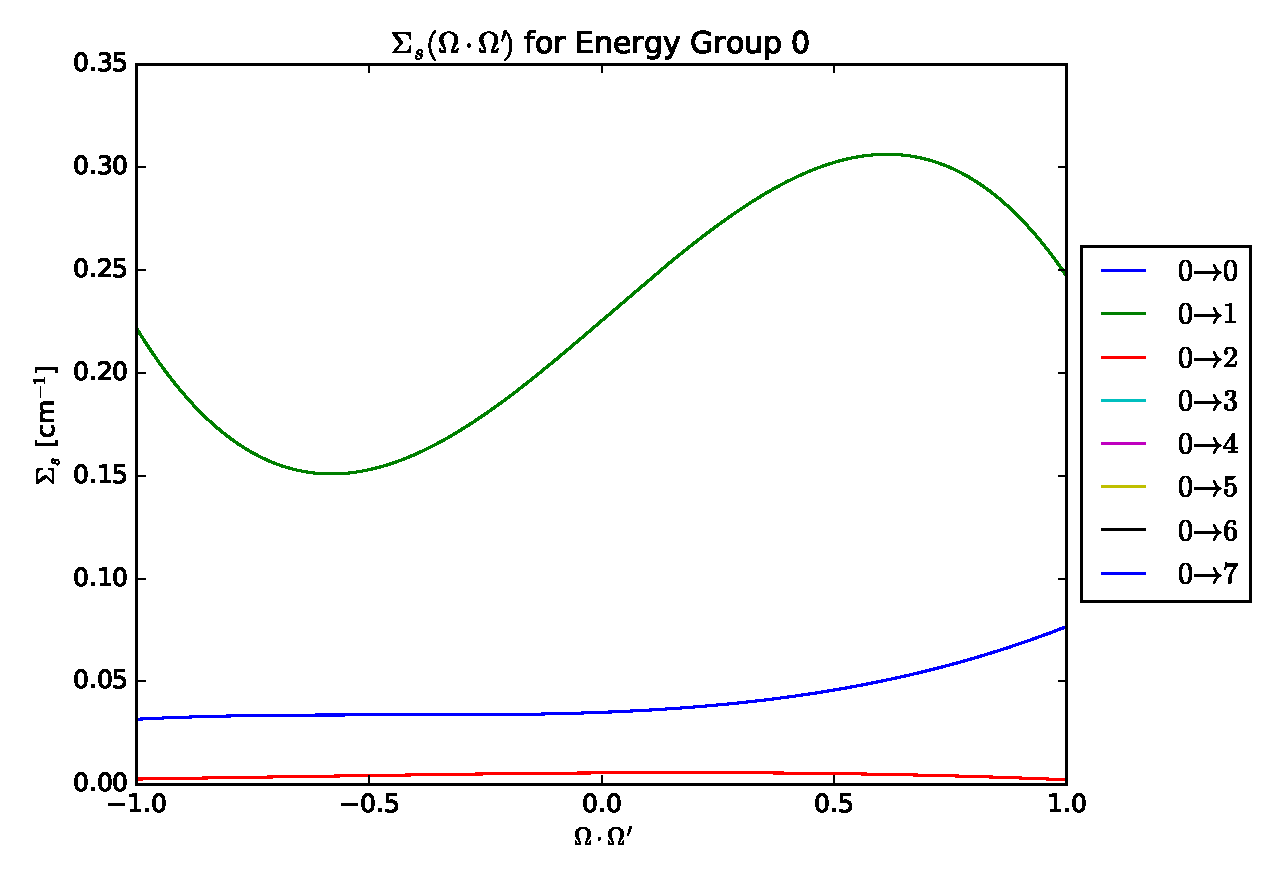
\includegraphics[width=\textwidth]{img/xs.eps}
\caption{Water scattering cross section as a function of angle in the highest energy group.}
\label{fig:water-xs}
\end{figure}
\FloatBarrier

In Figure \ref{fig:water-xs-coarse} we see that the coarse QR and LDO quadrature
sets both capture the forward-peakedness of this cross section. The QR quadrature set
contains fewer unique values of $\bo\cdot\bo'$ than does the LDO quadrature set,
however, and the LDO quadrature set produces values of $\Sigma_s$ that are closer to
the extremal values of the reference cross section curve. The potential impact of this
is the possibility of being able to use relatively coarse LDO quadrature sets in 
solving a problem while incorporating the problem's angular dependence better than a 
standard quadrature set of a similar coarseness would.

\begin{figure}[!htb]
\centering
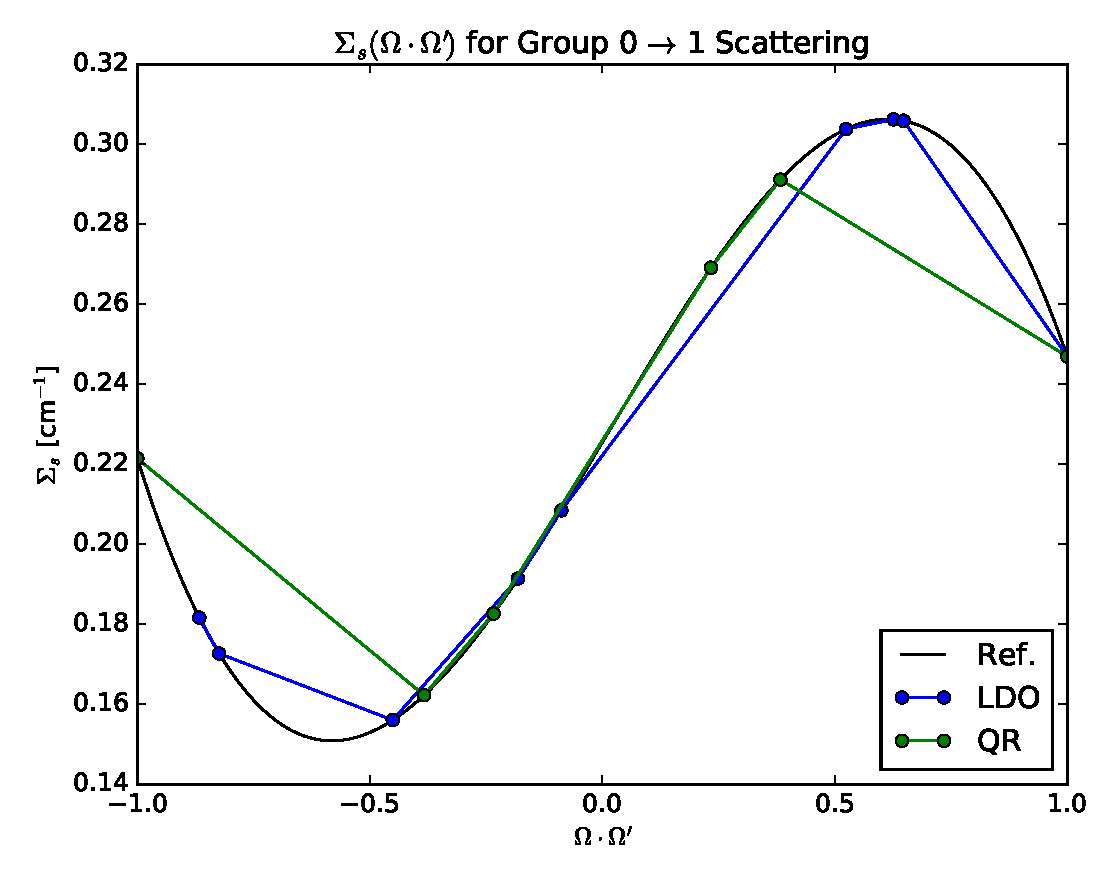
\includegraphics[width=\textwidth]{img/xs-coarse.eps}
\caption{Group 0 $\to$ 1 scattering cross section reconstructed with coarse angular meshes.}
\label{fig:water-xs-coarse}
\end{figure}
\FloatBarrier

Finer angular meshes of both quadrature set types are shown in Figure 
\ref{fig:water-xs-fine}; in this plot the QR quadrature set has 128 angles and the LDO 
quadrature set has 144 angles.
It is seen that both quadrature set types match the reference
cross section curve quite well when the angular mesh is refined. This is unsurprising
for the QR quadrature set and serves as a confirmation that the LDO formulation is 
formally the same as the traditional discrete ordinates equations.

\begin{figure}[!htb]
\centering
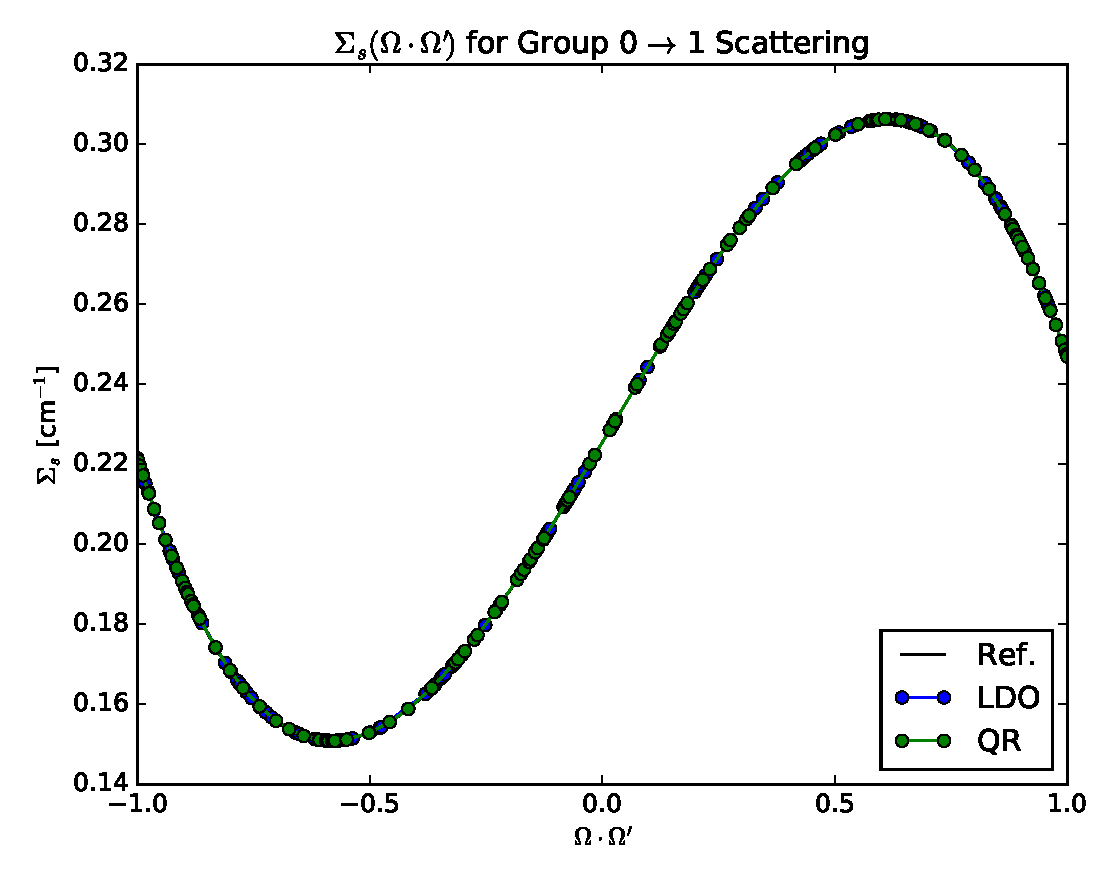
\includegraphics[width=\textwidth]{img/xs-fine.eps}
\caption{Group 0 $\to$ 1 scattering cross section reconstructed with fine angular meshes.}
\label{fig:water-xs-fine}
\end{figure}
% \FloatBarrier

\FloatBarrier
\subsection{Scattering in Denovo}

In Denovo and most other discrete ordinates codes, the operation $\mathbf{L}^{-1}$ in 
Equation \ref{l_inv} represents a sweep through the system mesh in the directions of 
particle travel \cite{denovo}. 
We can rewrite Equation \ref{l_inv} to reframe it as solving for the total source $Q$:

% eq 5 in the sweep sources pdf
\begin{equation}
Q = \ve{DL}^{-1}\left(\ve{M}Q_m + Q_d\right).
\label{swpsrc}
\end{equation}

\noindent Here, the operators are the same as those in Equation \ref{l_inv}, $Q_m$ is 
the sum of the ``moment-based'' sources, and $Q_d$ is the sum of the ``discrete'' 
sources \cite{sweepsources} as shown in Equation \ref{qmd}. Recalling Equation 
\ref{swpsrc}, moment-based sources are those to which the moment-to-discrete operator 
$\ve{M}$ is applied in the traditional discrete ordinates formulation. Discrete sources
are not operated on by $\ve{M}$ and may be restricted to a subset of the discrete 
angles used in a given problem.

\begin{equation}
Q_m = \sum_{s=1}^{S_m}Q_{m,s} \quad\text{ and }\quad Q_d = \sum_{s=1}^{S_d}Q_{d,s},
\label{qmd}
\end{equation}

\noindent where $Q_{m,s}$ is a particular moment-based sweep source, $Q_{d,s}$ is a
particular discrete-based sweep source, $S_m$ is the total number of moment-based 
sources in the system, and $S_d$ is the total number of discrete sources
\cite{sweepsources}. Figure \ref{swpsrclist} shows the sweep source hierarchy
implemented in Denovo, where the goal of the infrastructure is to calculate the total
source listed in Equation \ref{swpsrc} by performing a transport sweep over the 
combined particle sources.

\begin{figure}[!htb]
\centering
\includegraphics[width=\textwidth]{img/swp-src.png}
\caption{Sweep source hierarchy in Denovo \cite{sweepsources}.}
\label{swpsrclist}
\end{figure}

From this diagram, it is apparent that all scattering derives from a common base class,
the scattering sweep source base, and that this base class derives from the 
moment-based sweep source class.
The types of scattering supported include downscattering, within-group scattering,
upscattering, and first-collision scattering. The scattering classes share a great deal
of functionality, hence the implementation of the common base class. Because the
scattering sweep source is a type 
of moment-based sweep source, we note the particular difference in the operator
forms of the discrete ordinates and LDO formulations and how that translates into 
implementing scattering calculations in Denovo.

In the LDO formulation, the interpolation matrix $\mathbf{J}$ is applied to the 
moment-based sources. Looking at Equations \ref{l_inv} and 
\ref{ldo_op}, it is apparent that the operator order is different between the 
traditional discrete ordinates formulation and the LDO formulation, Namely, the product
of the scattering matrix and the moment-to-discrete or interpolation matrix is reversed
between the two sets of equations. To handle this difference, a ``scattering 
calculator'' was implemented in the scattering sweep source base class such that the
scattering sweep source is calculated in accordance with the formulation of the
equation set being solved.

\section{Selection of Quadrature Sets}

As mentioned in Section \ref{sec:ldo_math}, the LDO equations are developed with and
must be evaluated at a fundamental system of points for the subspace of spherical
harmonics. Ahrens provides references for examples of construction methods of these
point systems \cite{ahrens}. Like Ahrens, we have chosen to use the extremal point sets
developed and distributed by Womersley \cite{wom}.

Womersley's extremal systems are generated such that the associated Gram matrix is
positive definite \cite{wom}; these matrices are of interest to work with from an
implementation standpoint because of their low condition numbers. In Table \ref{md03}
we give an example of a point set generated by Womersley. The point set is of degree 3
and thus contains 16 points.

\begin{table}[!htb]
\centering
\caption{The ``md003.00016'' quadrature set developed by Womersley \cite{wom}.}
\small
\begin{tabular}{cccc}
\multicolumn{1}{c}{\textbf{$\mu$}} & 
\multicolumn{1}{c}{\textbf{$\eta$}} & 
\multicolumn{1}{c}{\textbf{$\xi$}} & 
\multicolumn{1}{c}{\textbf{$w$}} \\
\hline
0.00000000000000000 & 0.0000000000000000 & 1.0000000000000000 &
0.73999377643692810 \\
0.89273429807179527 & 0.0000000000000000 & -0.45058348066286125 &
0.73999377643692787 \\
-0.14301510478336188 & 0.98579910306911467 & -0.088015954189755163 &
0.73999377643692688 \\
-0.73214276086495222 & 0.51082433836573149 & -0.45058348066286003 &
0.73999377643692854 \\
0.65748213697787805 & -0.7831172071742225 & -0.088015954189756496 &
0.73999377643692765 \\
-0.70626478165373330 & 0.4595590936077425 & 0.52407635945553088 &
0.92161132427900849 \\
-0.60670408850507063 & -0.4914548265981833 & 0.62661538904237324 &
0.73999377643692887 \\
-0.29492456926406690 & -0.9812320737717869 & -0.18150577463199227 &
0.92161132427900960 \\
0.21767572867043725 & -0.7831172071742269 & 0.62661538904237279 &
0.73999377643692787 \\
-0.51446703219451573 & -0.23748738235169115 & -0.82396809162048790 & 
0.73999377643692743 \\
0.85155965361038066 & -0.013788611344369470 & 0.52407635945553044 &
0.92161132427900860 \\
0.28603020956672459 & -0.48914548265981850 & -0.82396809162048790 &
0.73999377643692776 \\
0.14962969730741976 & 0.47595590936077353 & -0.86664694427906974 &
0.92161132427900883 \\
-0.96739492195887000 & -0.23748738235169184 & -0.088015954189756274 & 
0.73999377643692821 \\
0.68136471239214502 & 0.72663286501151070 & -0.088015954189756274 &
0.73999377643692898 \\
0.22843682262779150 & 0.72663286501151014 & 0.64793618324097579 &
0.73999377643692754
\end{tabular}
\label{md03}
\end{table}

We note that all of Womersley's extremal systems are generated such that the first
point in each set is situated along the $z$-axis. These systems are rotationally
invariant with respect to the maximization of the logarithm of the determinant of the 
associated Gram matrix, so the point sets may be rotated in space if this vector
placement is undesirable for a given scenario. The work presented and discussed in 
Chapter \ref{sec:results} uses the point sets posted by Womersley; exploration of using
rotated extremal point sets is a potential area of future work.

\section{Restrictions}

Several restrictions exist for solving the LDO equations in the Exnihilo framework as
well as employing the solutions in the ADVANTG software. Some of these restrictions are
a result of implementing the LDO equations in a framework designed to solve the
traditional discrete ordinates equations, while other restrictions are merely 
current limitations of the software pieces used in this work.

\subsection{Boundary Conditions}
\label{sec:bc}

Although it is mathematically possible to use reflective boundary conditions for the
LDO equations (given their interpolatory nature), the current implementations of the
various codes used in this work restrict the solutions to vacuum (black) boundary
conditions at the time of this writing. The primary reason for this is that the
ADVANTG software does not support the use of reflective boundary conditions, and the
LDO equations were implemented into the Exnihilo framework for the purpose of using 
the solutions in ADVANTG for Monte Carlo variance reduction parameter generation. To a
lesser extent, the Exnihilo framework was built with symmetric quadrature sets in mind,
and so the use of reflective boundary conditions with the LDO equations was considered
to be an effort beyond the scope of this work.

\subsection{Uncollided Flux}
\label{sec:uncflux}

The use of an ``analytic'' approximation of the uncollided flux source,
a method employed to reduce ray effects from point sources or other small sources
\cite{exum}, is not available when solving the LDO equations through Exnihilo. This
approximation is obtained in Denovo by solving the following equations for the group
uncollided flux moments for every mesh cell in the calculation domain:

\begin{equation}
\bo\cdot\nabla\psi^g(\bo) + \sigt^g\psi^g(\bo) = \frac{Q^g_p}{4\pi}\delta(r-r_p),
\label{uncflux_eq}
\end{equation}

\noindent where $|r-r_p|$ is the geometric distance between the flux source and some
particular point and the analytic solution of the above equations is

\begin{equation}
\psi^g(\bo) = \delta(\bo - \bo_{p\rightarrow r})\frac{Q^g_p}{4\pi|r-r_p|^2}
e^{-\tau(r,r_p)}.
\label{uncflux_sln}
\end{equation}

\noindent In Equation \ref{uncflux_sln}, the term $\delta(\bo - \bo_{p\rightarrow r})$
indicates that the angular flux at a given point is only nonzero for the the angle that
passes directly from the source through the particular point of interest. The ``optical
path length'' $\tau(r,r_p)$ is the integral of the total cross section from the 
source location to the point of interest and is calculated via ray tracing.

Because the Exnihilo framework was written to solve the traditional form of 
the discrete ordinates equations, these flux moment solutions in Equation
\ref{uncflux_sln} are based on the expansion listed in Equation \ref{sph_harm_exp}.
That is to say, when using the analytic uncollided flux approximation, the flux moments
are calculated using the components of the spherical harmonic functions listed in
Equations \ref{eq:sph_e} and \ref{eq:sph_o}. So, the solutions do not apply to the LDO
equations and this treatment cannot be used. All tests in the following chapter were
run with the uncollided flux treatment turned off; implementing this approximation for
use with the LDO equations in Denovo remains an area of future work.

\subsection{Particle Sources}
\label{sec:ptsrc}

When considering neutron transport problems of interest, a small variety of particle 
source types appear frequently. One typical source type is an isotropic source, in 
which particles are emitted uniformly in all directions. Specifically, isotropic point 
sources, in which the physical size of the source itself is negligible, are routinely 
used in both experimental work and simulations.

Point sources must be approximated as small volumetric sources when solving the LDO
equations in Denovo. When a point source is used in a system, Denovo calculates the
uncollided flux from that point source using the analytic solution to the NTE. As
mentioned previously, this is done to alleviate ray effects. However, as discussed 
above in Section \ref{sec:uncflux}, these analytic solutions are not applicable when
solving the LDO equations. Thus, when a point source is specified in combination with 
the LDO equations, it is treated as a small volume source instead. In this case, an
equal contribution of the source strength is added to every angular flux coefficient in
the cell in which the particle source resides. This is notably different from the
traditional discrete ordinates formulation in Denovo, in which the source strength is
added only to the zeroth flux moment for reasons described in Section \ref{sec:flux}.

Finally in this section, we note that this work is limited to isotropic particle
sources. At the time of this writing, ADVANTG does not support directional sources 
\cite{munk}; Monte Carlo particle importance maps generated with ADVANTG and Denovo
automatically use an isotropic source distribution regardless of the particle source
input. Since the ultimate goal of implementing the LDO equations in the Exnihilo
framework is to use the results for Monte Carlo variance reduction parameter 
generation via ADVANTG, implementation of the use of directional sources when solving 
the LDO equations in Denovo was not pursued in this work.

\subsection{Fixed Source vs. Criticality Calculations}

All scenarios tested in this work are fixed-source problems, though the LDO equations
are applicable to $k$-eigenvalue (criticality) problems in principle. Ray effects,
which we are interested in using solutions of the LDO equations to mitigate, largely
come from localized sources, as discussed in Section \ref{sec:ray}. Due to the 
distributed nature of fission sites in a typical light water reactor, the particle 
flux in a given criticality calculation will be relatively isotropic and unlikely to 
incur ray effects within the reactor core. Furthermore, at the time of this writing, 
ADVANTG only supports generation of Denovo input for fixed-source problems. 

\chapter{Test Cases and Results}
\label{sec:results}

In this chapter we present the test case scenarios simulated in this work as well as
the results of the various simulations performed. First, a description of the 
scenarios is given to detail the geometry and cross section configurations used. 
Next, a comparison of deterministic results for the test scenarios is given, with 
discussion and emphasis placed on the difference in the results between different 
types of quadrature sets. Then, we present results and analysis of the performance of
the quadrature sets' associated Monte Carlo variance reduction parameters in the
context of both CADIS and \fwc\ simulations. Finally, a summary of the results is
given to conclude the chapter.

\section{Test Case Scenarios}

\subsection{Steel Plate in Water}
\label{sec:steel_params}

The first test case we describe is an idealized geometry of a steel plate embedded in
water; it is modeled after the scenario presented in Reference 
\cite{wilsonslaybaugh}. 
A diagram of the problem geometry is shown in Figure \ref{steelxz} and a list
of material properties used in the problem is given in Table \ref{steel-mat}.
In Figure \ref{steelxz}, the orange region contains the source material, the black
region is composed of steel, the blue regions indicate water, and the white region is
composed of air.

\begin{figure}[!htb]
\centering
\includegraphics[width=0.4\textwidth]{img/steel-xz.png}
\caption{Steel plate in water geometry ($x-z$ slice through $y = 25$ cm) 
         \cite{wilsonslaybaugh}.}
\label{steelxz}
\end{figure}

The problem measurements are $53\times50\times140$ cm. The scenario is uniform in the 
$y$-direction and materials vary mainly in the $z$-direction. The source region 
extends from 0 to 15 cm, the steel shield extends between 15 and 30 cm, the water and 
steel plate extend from 30 to 130 cm, and the air extends from 130 to 140 cm. The 
steel plate is 3 cm wide and is centered at $x = 26.5$ cm. Vacuum boundary conditions 
were used at the problem boundaries.

A non-uniform Cartesian mesh was used for the spatial discretization in the 
deterministic calculations. In the $x$-direction, voxel width is 5 cm between $x = 0$
cm and $x = 25$ cm, 0.5 cm between $x = 25$ cm and $x = 28$ cm, and 5 cm between 
$x = 28$ cm and $x = 53$ cm. A uniform spacing of voxel width 1 cm was used in the 
$y$-direction. In the $z$-direction, the spatial cell width is 3 cm between $z = 0$ cm and
$z = 30$ cm and 2 cm between $z = 30$ cm and $z = 140$ cm.

\begin{table}[!htb]
\centering
\caption{Materials and compositions in the steel plate in water scenario.}
\label{steel-mat}
\begin{tabular}{l|cc}
\textbf{Material} & \multicolumn{2}{c}{\textbf{Isotopes (Atomic \%)}} \\ \hline
\multirow{5}{*}{Source}   & U-235   & (0.000247) \\
                          & U-238   & (0.009287) \\
                          & Zr-nat. & (0.004009) \\
                          & H-1     & (0.037394) \\
                          & O-16    & (0.034927) \\ \hline
\multirow{4}{*}{Air}      & N-14    & (0.784431) \\
                          & O-16    & (0.210748) \\
                          & Ar-nat. & (0.004671) \\
                          & C-nat.  & (0.000150) \\ \hline
\multirow{2}{*}{Carbon Steel} & C-nat.  & (0.022831) \\
                              & Fe-nat. & (0.977169) \\ \hline
\multirow{2}{*}{Water}        & H-1     & (2)        \\
                              & O-16    & (1)        \\
\end{tabular}
\end{table}

The composition of the neutron source block is a homogenization of water, zirconium,
and uranium and was calculated based on the geometry and composition of the Rowlands
UO$_2$ pin cell benchmark specification \cite{pincell}. The source is a U-235 fission 
spectrum that is uniformly distributed throughout the homogenized material. The
compositions of air, carbon steel, and water were taken from the Compendium of 
Material Composition Data for Radiation Transport Modeling \cite{pnnl}. For this scenario,
we are interested in the forward flux solutions at the end of the steel plate.

\FloatBarrier
\subsection{Dog-Legged Void Neutron (DLVN)}

The next problem modeled is the dog-legged void neutron (DLVN) experimental benchmark,
which was designed to measure neutron streaming in iron with air voids. The model used
in the following calculations was constructed from References 
\cite{sw-dlvn,j-dlvn,dlvn1991}. The two materials used in the problem are elemental 
iron and polyethylene. The polyethylene composition used was C$_2$H$_4$. This is 
listed as ``polyethylene, non-borated'' and is material 248 in Reference \cite{pnnl}. 

\begin{figure}[!htb]
\centering
\includegraphics[width=0.5\textwidth]{img/dlvn.png}
\caption{Centerline cutaway of DLVN setup \cite{sw-dlvn}.}
\label{dlvn}
\end{figure}

The problem measurements are $40\times54\times48$ inches. A uniform spatial mesh was 
imposed over the entire problem, with voxels measuring 1 inch per side. The neutron
source in this problem is a Cf-252 point source located at the center of the $x-$ and
$y-$directions and at $z = 9$ inches. For reasons noted in Section \ref{sec:ptsrc},
this point source was approximated as a small volumetric source in the tests in this 
work. We are interested in the forward flux solutions at the various detector locations
shown in Figure \ref{dlvn}.

The experimental configuration is symmetric about the $y-z$ plane at $x = 0$ and so is
usually simulated with a reflecting boundary at $x = 0$ and vacuum boundaries on all
other sides of the configuration. For the tests in this work, the use of reflecting
boundary conditions was not available (see Section \ref{sec:bc}), so the model used 
was constructed to represent the entire experimental geometry configuration. Vacuum
boundary conditions were applied to the outside of the entire problem.

\FloatBarrier
\subsection{Ispra Sodium Benchmark}

The Ispra sodium benchmark experiment was constructed as part of experiments to study
neutron deep penetration in homogeneous materials commonly used in advanced nuclear
reactors. It is included in the Shielding Integral Benchmark Archive and Database 
(SINBAD) data library \cite{sinbad}. We will give a brief overview of the material and
geometry configuration here and refer the reader to Reference \cite{sinbad} for a 
complete description of the experiment.

The neutron source consists of fission neutrons originating from an enriched U disc 
that was subjected to a neutron flux leaving the thermal column of a TRIGA MARK II 
reactor. An irradiation tunnel assembly composed of steel containers filled with Na 
was constructed in front of the neutron source converter. The total length of the 
irradiation tunnel was 400 cm. A diagram of the experimental geometry is shown in 
Figure \ref{eurac}; we are interested in the forward flux solutions in the detector
array located along the midline of the assembly.

\begin{figure}[!htb]
\centering
\includegraphics[width=\textwidth]{img/eurna-2v.png}
\caption{Cross sectional views of the sodium benchmark assembly.}
\label{eurac}
\end{figure}

In the simulation of this benchmark configuration, the boundaries are -300 cm and 500
cm in the $x-$direction and -400 and 400 cm in both the $y-$ and $z-$directions.
The spatial mesh in this problem is uniform in the $y-$ and $z-$directions with a 
voxel width of 5 cm per side in these dimensions. The $x-$direction mesh was 
created such that voxels are 10 cm wide between $x =$ -300 and -100 cm, 5 cm wide 
between $x =$ -100 and 400 cm, and 10 cm wide between $x =$ 400 and 500 cm. The problem
has vacuum boundary conditions.

\FloatBarrier
\subsection{Simplified Portal Monitor}

The final problem described here is a simplified portal monitor scenario. Portal
monitors are large detector panels used to screen cargo for illicit radioactive
materials. The problem models a cargo container holding a Ba-133 photon point source
and large blocks of homogenized iron and polyethylene. 
The geometry and material configuration used in this test is the same as the
example problem listed in Section 7.2 of the ADVANTG technical report \cite{advantg};
slight modifications were made to the given MCNP input deck such that the problem 
could be studied with both CADIS and \fwc\ calculations. Diagrams of the simplified 
portal monitor problem are shown in Figure \ref{p1}.

\begin{figure}[!htb]
\centering
\begin{subfigure}{0.475\textwidth}
\includegraphics[width=\textwidth]{img/portal1.png}
\end{subfigure}
\begin{subfigure}{0.475\textwidth}
\includegraphics[width=\textwidth]{img/portal2.png}
\end{subfigure}
\caption{Top and side views of simplified portal problem \cite{advantg}.}
\label{p1}
\end{figure}

In Figure \ref{p1}, the different colors represent different materials. The NaI 
detectors are red and the gray material is concrete. The two types of material blocks
are iron, shown in green, and polyethylene, shown in white. The steel cargo container
surrounds the particle source and material blocks and is a semitransparent blue. Here
we are interested in the forward flux solutions at the four detector locations.

A non-uniform Cartesian mesh that captures all of the problem's material boundaries
was constructed for this simulation. The voxels are nominally 10 cm thick within the
cargo container. Additional mesh planes parallel to the $x-$axis were added to the 
gaps between the homogenized iron and polyethylene blocks \cite{advantg}. Vacuum
boundary conditions are present at all problem edges.

\subsection{Calculation Parameters}
\subsubsection{Deterministic}
\label{params}

All of the deterministic calculations used 32 processes on a 2.8GHz AMD 
Opteron\texttrademark\ 6320 Processor \cite{amd}, two for each logical CPU unit. 
With this in mind, all deterministic calculations were set to use the same Denovo 
computational block structure of 8 blocks 
in the $x-$dimension, 4 blocks in the $y-$dimension, and 1 block in the $z-$dimension;
thus the total number of computational blocks equals the number of processes.
Denovo uses the Koch-Baker-Alcouffe (KBA) parallel sweep algorithm for high
parallel efficiency in calculating transport sweeps \cite{denovo}; the aforementioned
block structure was chosen to achieve the same parallel decomposition among all test 
case deterministic simulations. 

All but one of the test cases use the same coarse energy group structure specified in 
the ``27n19g'' library; the groups in this library are listed in Table A-1 of 
Appendix A of the ADVANTG technical report \cite{advantg}. The exception to this is 
the simplified portal problem. The highest energy emission line of Ba-133 is 383.8 
keV, so weight window bounds above this energy would not be used in the Monte Carlo 
simulation. Thus, the highest energy group of the deterministic calculations was set 
to group number 41, which has an upper energy of 400 keV \cite{advantg}. Because 
energy discretization is treated the same way between the traditional discrete 
ordinates formulation and the LDO equations, it was assumed that energy group 
structure would not greatly impact the comparative results.

The step characteristics (SC) spatial discretization was used in all of the
deterministic calculations based on the recommendation listed in Section 9.1.3 of the
Exnihilo user manual \cite{exum}. In the DLVN and portal monitor scenarios, the point
sources are approximated as small spherical volumetric sources (see Section 
\ref{sec:ptsrc} for detail).

Except for the Galerkin quadratures, all runs used a P$_5$ scattering expansion. At 
the time of this writing, Galerkin quadrature sets are implemented in the Exnihilo 
framework with the restriction that the \pn order be one greater than the \sn order.
That is, for the Galerkin quadrature set of \sn order 2, the corresponding \pn order 
is set equal to 3, and for the Galerkin quadrature set of \sn order 4, the \pn order
is 5.

\subsubsection{Monte Carlo}
\label{mcparams}

The Monte Carlo calculations in this work were run on one Dell PowerEdge C6220
server  blade node with two Intel Xeon 10-core Ivy Bridge processors (a total
of 20 cores) \cite{savio}. All calculations were specified to use 21 MPI
tasks; MCNP reserves one ``master'' process for communication and transports
particles with the remaining available tasks \cite{mcnp}. So, for the purpose
of parallel efficiency, one transport process per hardware core was used here.

All of the Monte Carlo calculations were run with a fixed number of particle 
histories to simulate. For the steel plate in water, Ispra sodium benchmark, and 
simplified portal monitor cases, all calculations used 1\E{9} particle histories in 
both the CADIS and \fwc\ contexts. The DLVN experimental benchmark case was simulated 
with 1\E{10} neutron histories as it was modeled after calculations in Reference 
\cite{sw-dlvn}. All Monte Carlo tally results and following calculations
are reported with the one standard deviation confidence interval $\xbar(1\pm R)$ where the
relative error $R \equiv S_{\xbar}/\xbar$ \cite{mcnp}.

\FloatBarrier
\section{Deterministic Forward Flux Calculations}
\label{sec:det-fwd}

Before investigating deterministic flux solutions resultant from solving the LDO
equations as input for Monte Carlo variance parameter generation, it behooves us to
compare the LDO deterministic results against those of standard quadrature set types.
We start here by presenting results and analysis for forward scalar flux solutions
using different quadrature types for the four test cases. We assume extensibility of
these results to adjoint scalar flux solutions since the changes to the Exnihilo code
suite made in this work did not impact the transport solvers in the Denovo package.

For all of the quadrature set types and sizes discussed above, a forward simulation of
each test case was run via the Exnihilo framework. The following results show a
representative quadrature set chosen for each type. With the exception of the 
Galerkin quadrature set featured, the angular refinement of the representative 
quadrature sets was chosen such that the quadrature sets have approximately the same 
total number of angles. The QR quadrature set is of order 4 and has 128 angles, the 
LDFE set is order 1 with 128 angles, and the LDO set is of order 11 with 144 angles. 
The Galerkin quadrature set chosen as the representative example here is of order 4 
and has 24 angles. This set was chosen because its corresponding \pn order is 5 and so
the scattering data used matches that of the other quadrature types.

Because more results were generated than are presented here, a fuller set of figures 
is hosted at \url{http://dx.doi.org/10.6084/m9.figshare.6063053}.

\subsection{Quadrature Sets}

In these preliminary deterministic calculations, forward solutions for the test cases
were generated using quadruple range (QR), Galerkin, linear-discontinuous finite 
element (LDFE), and LDO quadrature sets. All test cases were run with the same 
quadrature sets; increasing sizes of quadrature sets were used to ascertain the
angular mesh refinement necessary for a given quadrature type to converge to a 
solution. 

QR quadrature sets were chosen to generate the reference results against which the 
LDO results are compared. QR was selected because they are commonly used 
in hybrid methods for Monte Carlo variance reduction parameter generation and 
therefore provide a relevant baseline. The Exnihilo
framework allows the user to select the number of polar and azimuthal angles in each
octant when using a QR quadrature set; for these studies, the number of polar and 
azimuthal angles per octant were each set to the same value, with the values ranging
from one per octant (for a total of eight angles) to nine per octant (for a total of
648 angles). 

LDFE and Galerkin quadrature sets were also chosen because of their interesting 
mathematical properties. Compared to QR quadrature sets, LDFE quadrature sets have 
been shown to exhibit more accurate solutions for the scalar flux in both 
simple and more complex geometry and material configurations \cite{ldfe}; they 
approximate the angular flux using direction cosines and are determined by requiring 
that the integration of the related interpolation basis functions is equal to the 
surface area of a unit sphere. For LDFE quadrature sets, if $N$ is the order of the 
quadrature, there are $4^{(N+1)}$ angles per octant \cite{exum}. In this work, the 
LDFE quadrature orders used were one (128 total angles) and two (8192 total angles).

Galerkin quadrature sets offer several advantages relative to the standard \sn method
for problems with highly anisotropic scattering \cite{morel}. Similar to the LDO
equations, the ``hybrid collocation-Galerkin-S$_\mathrm{N}$'' method developed by 
Morel has the same algebraic structure as the traditional discrete ordinates 
equations but employs a nonstandard scattering treatment.
For reasons discussed below in Section \ref{params}, the Galerkin quadrature orders
used were 2 and 4. For an \sn order $N$, a given Galerkin quadrature set (as
implemented in Exnihilo) has a total of $N(N+2)$ angles; the Galerkin quadrature sets
used in this work have 8 and 24 total angles, respectively.

The degrees and sizes of the LDO quadrature sets used are listed in Table
\ref{ldo-n}.

\begin{table}[!htb]
\centering
\caption{Properties of LDO quadrature sets used in preliminary scaling studies.}
\begin{tabular}{cc}
\multicolumn{1}{l}{\textbf{Quadrature Order ($\mathbf{N}$)}} & 
\multicolumn{1}{l}{\textbf{Number of Points}} \\
\hline
3 & 16 \\
5 & 36 \\
8 & 81 \\
9 & 100 \\
11 & 144 \\
12 & 169 \\
13 & 196 \\
14 & 225 \\
\end{tabular}
\label{ldo-n}
\end{table}

\FloatBarrier
\subsection{Steel Plate in Water}
\label{sec:steel-fwd}

Figure \ref{steel-fwd-slices} shows a representative forward scalar flux slice plot 
for each quadrature type. Each of the flux slices is at the midplane of the 
$y-$dimension such that $y = 25$ cm. The geometry/material borders are outlined on
each plot as well. All plots show the same expected result -- the scalar flux is 
highest in the source region and drops off by orders of magnitude along the $z-$axis.

To more thoroughly evaluate the LDO quadrature set in this test case, we will look 
more closely at the differences between the representative LDO flux and the three
other quadrature types. Figure \ref{steel-fwd-diff-rel} shows three plots of relative
flux differences; each plot compares the representative LDO quadrature set against one
of the standard quadrature set types. The relative flux difference is calculated as

\begin{equation}
\phi_{\mathrm{diff}} = 
\frac{\left|\phi_{\mathrm{LDO}}-\phi_{\mathrm{ref}}\right|}{\phi_{\mathrm{ref}}}
\label{flux-diff}
\end{equation}

\noindent where $\phi_{\mathrm{ref}}$ is the scalar flux calculated using the 
standard quadrature set and is taken to be the reference value. For all three of the
standard quadrature sets, the area of greatest agreement with the LDO scalar flux is
towards the bottom of the problem geometry, with discrepancies growing along the
$z-$axis. The greatest difference can be seen between the LDO and Galerkin quadrature 
sets, while the LDO and QR quadrature sets agree best. The area of greatest
discrepancy between the QR and LDO flux solutions is in the region of air just beyond
the steel beam. We will look more in depth as to why this is in Section 
\ref{sec:steel-cad} and briefly note here that this particular deviation is most 
likely due to issues in processing iron cross section data inherent to deterministic
calculations.

Table \ref{steel-fwd-diff-table} lists the minimum, maximum, and average differences
between various quadrature types for the flux slices plotted in Figure 
\ref{steel-fwd-diff-rel}. We compare the representative LDO flux solution to the 
solutions from the three standard representative quadrature types and also
compare the Galerkin and LDFE results against the QR result. On average, the LDO
forward flux solution matches the QR flux solution more closely than it matches either
the Galerkin or LDFE flux solutions. Additionally, the LDO flux solution matches the
QR flux solution more closely than do either of the Galerkin and LDFE flux solutions.

\begin{table}[!hbt]
\centering
\caption{Steel plate forward scalar flux extremal and average relative differences.}
\label{steel-fwd-diff-table}
\begin{tabular}{l|ccc}
\textbf{Comparison} & \textbf{Min. Diff.} & \textbf{Max. Diff.} & \textbf{Avg. Diff.} 
\\ \hline
LDO/QR              & 6\E{-6}             & 1.09\E{-1}       & 2.21\E{-2}
\rule{0pt}{2.6ex} \\ 
LDO/Galerkin        & 2\E{-5}             & 4.51\E{0}        & 9.30\E{-1}      \\
LDO/LDFE            & 5\E{-7}             & 2.79\E{-1}       & 9.42\E{-2}      \\
Galerkin/QR         & 3\E{-5}             & 8.24\E{-1}       & 2.90\E{-1}      \\
LDFE/QR             & 2\E{-7}             & 2.48\E{-1}       & 9.63\E{-2}
\end{tabular}
\end{table}

Looking at Figures \ref{steel-fwd-slices} and \ref{steel-fwd-diff-rel} we note that
the forward scalar flux solutions from the LDO equations capture the same physical
trends as the standard quadrature type solutions and also that the LDO flux solution
most closely matches that using the QR quadrature set. Additionally, Table 
\ref{steel-fwd-diff-table} shows an average difference of 2.2\% between the
plotted flux solutions from the representative LDO and QR quadrature sets, which is 
the lowest average difference seen in the comparisons here. As QR quadratures are 
commonly used for Monte Carlo variance reduction parameter generation, the relative 
agreement of the LDO scalar flux with the QR scalar flux motivates the exploration of 
the use of LDO scalar flux solutions for Monte Carlo variance reduction parameter 
generation.

\begin{figure}[!htb]
\centering
\begin{subfigure}{0.4\textwidth}
\includegraphics[max height=0.445\textheight]
{img/steel-plots/fwd/flux-qr04-slice.eps}
\subcaption{QR forward flux slice.}
\end{subfigure} ~
\begin{subfigure}{0.4\textwidth}
\includegraphics[max height=0.445\textheight]
{img/steel-plots/fwd/flux-gkn04-slice.eps}
\subcaption{Galerkin forward flux slice.}
\end{subfigure}
\\
\begin{subfigure}{0.4\textwidth}
\includegraphics[max height=0.445\textheight]
{img/steel-plots/fwd/flux-ldfe01-slice.eps}
\subcaption{LDFE forward flux slice.}
\end{subfigure} ~
\begin{subfigure}{0.4\textwidth}
\includegraphics[max height=0.445\textheight]
{img/steel-plots/fwd/flux-ldo11-slice.eps}
\subcaption{LDO forward flux slice.}
\end{subfigure}
\caption{Steel plate forward scalar flux slices.}
\label{steel-fwd-slices}
\end{figure}

\begin{figure}[!htb]
\centering
\begin{subfigure}{0.4\textwidth}
\includegraphics[max height=0.445\textheight]
{img/steel-plots/fwd/flux-diff-rel-qr04.eps}
\subcaption{LDO/QR flux rel. diff.}
\end{subfigure} ~
\begin{subfigure}{0.4\textwidth}
\includegraphics[max height=0.445\textheight]
{img/steel-plots/fwd/flux-diff-rel-gkn04.eps}
\subcaption{LDO/Galerkin flux rel. diff.}
\end{subfigure}
\\
\begin{subfigure}{0.4\textwidth}
\includegraphics[max height=0.445\textheight]
{img/steel-plots/fwd/flux-diff-rel-ldfe01.eps}
\subcaption{LDO/LDFE flux rel. diff.}
\end{subfigure}
\caption{Steel plate forward scalar flux relative difference slices.}
\label{steel-fwd-diff-rel}
\end{figure}

\FloatBarrier
\subsection{DLVN}

For the DLVN test case, we present flux slice plots for the same representative
quadrature sets listed in Section \ref{sec:steel-fwd}. Although the entire DLVN
experimental geometry was simulated, here we plot only half of the configuration; this
is the typical view of the benchmark seen in the literature.

Figure \ref{dlvn-fwd-slices} shows the forward scalar flux for each of the
representative quadrature sets at the midplane of $y = 27$ inches (68.58 cm). Each of 
the plots has outlines of the material boundaries with the detector locations 
delineated as well. As expected, the flux is highest at the neutron source and 
decreases as particles move through the experimental configuration.
With this, we again look at the differences between the representative LDO flux and 
the three other quadrature types. 

As with the previous test case, the flux differences 
are calculated with Equation \ref{flux-diff}. In the DLVN scenario, the 
differences stem from the source location. This is not surprising; the particle source
here is approximately a point source and so these differences are appearing in the
form of ray effects, where the discrete angles in the LDO quadrature set do not 
overlap with the angles in a given standard quadrature set. Similar to the steel plate
in water test case, the LDO scalar flux best matches the QR scalar flux and the
largest differences are seen between the LDO and Galerkin scalar flux plots. Looking
at Figure \ref{dlvn-fwd-diff-gkn}, the areas of greatest discrepancy appear as ray
effects; the relative coarseness of the representative Galerkin quadrature set angular
mesh is likely the cause of this. This is visibly pronounced in the DLVN case because
of the geometrically small particle source; it is also likely the source of the 
LDO/Galerkin discrepancy seen above for the steel plate embedded in water, but ray
effects are lessened in that scenario by the larger volumetric source.

Lastly, it is instructive to compare the results of the forward deterministic scalar
flux solutions with the experimentally measured flux values at the detector locations.
Table \ref{dlvn-fwd-det} lists the experimentally measured \cite{dlvn1991} and
deterministically calculated scalar flux values at the detector locations noted in 
Figure \ref{dlvn}. Table \ref{dlvn-fwd-det-diff} lists the percent differences 
between the deterministically calculated flux values and experimentally determined 
flux values with the lowest difference for each detector location emphasized.

\begin{table}[!htb]
\centering
\caption{DLVN benchmark experimental and simulated scalar flux values [n/cm$^2$/s].}
\label{dlvn-fwd-det}
\begin{tabular}{l|ccccccc}
              & Det. \#5       & Det. \#9       & Det. \#11      & Det. \#12
              & Det. \#13      & Det. \#14 \\ \hline
Exp. Flux     & 6.97\E{-8}     & 1.57\E{-7}     & 8.81\E{-6}     & 2.60\E{-7}
              & 1.42\E{-6}     & 2.74\E{-7}     \rule{0pt}{2.6ex} \\
QR            & 4.98\E{-8}     & 1.68\E{-7}     & 8.65\E{-5}     & 4.92\E{-7}
              & 2.71\E{-6}     & 1.45\E{-6}     \\
Galerkin      & 3.24\E{-8}     & 1.47\E{-7}     & 8.19\E{-5}     & 4.43\E{-7}
              & 2.95\E{-6}     & 9.55\E{-7}     \\
LDFE          & 5.12\E{-8}     & 1.76\E{-7}     & 9.17\E{-5}     & 5.14\E{-7}
              & 2.93\E{-6}     & 1.47\E{-6}     \\
LDO           & 4.56\E{-8}     & 1.39\E{-7}     & 7.88\E{-5}     & 4.28\E{-7}
              & 2.37\E{-6}     & 1.28\E{-6}
\end{tabular}
\end{table}

\begin{table}[!htb]
\centering
\caption{Percent differences between DLVN experimental and simulated scalar flux 
         values.}
\label{dlvn-fwd-det-diff}
\begin{tabular}{l|ccccccc}
              & Det. \#5       & Det. \#9        & Det. \#11       & Det. \#12
              & Det. \#13      & Det. \#14       \\ \hline
QR            & \textbf{25.58} & 6.89            & 881.94          & 89.09
              & 90.63          & 428.81          \\
Galerkin      & 53.48          & \textbf{6.37}   & 829.72          & 70.56
              & 107.7         & \textbf{248.42} \\
LDFE          & 26.61          & 12.3           & 940.41          & 97.75
              & 106.4         & 435.01          \\
LDO           & 34.61          & 11.2           & \textbf{794.75} & \textbf{64.46}
              & \textbf{66.77} & 368.24
\end{tabular}
\end{table}

Looking at Table \ref{dlvn-fwd-det-diff} we see that all of the calculated values fall
outside of the experimental uncertainty of five percent \cite{dlvn1991}. The
results from the LDO quadrature set most closely match the experimental results for
half of the detector locations. This begs the question of how the LDO equations would
perform in the context of the \fwc\ method for the DLVN problem since the adjoint
source can be set to multiple detector locations. Table \ref{dlvn-fwd-diff-table}
lists the extreme and average values of the forward flux relative difference slices
shown in Figure \ref{dlvn-fwd-diff-rel} with Galerkin/QR and LDFE/QR comparisons
included for reference. We see that, on average, the LDO forward flux
solution matches the QR forward flux solution better than it matches those of the other
quadrature types. However, in this case, the LDFE flux solution matches the QR flux solution
on average better than any other quadrature type, including the LDO flux solution
(5\% difference versus 8.4\% difference).

\begin{table}[!hbt]
\centering
\caption{DLVN benchmark forward scalar flux extremal and average relative 
         differences.}
\label{dlvn-fwd-diff-table}
\begin{tabular}{l|ccc}
\textbf{Comparison} & \textbf{Min. Diff.} & \textbf{Max. Diff.} & \textbf{Avg. Diff.} 
\\ \hline
LDO/QR              & 2\E{-4}             & 8.40\E{-1}  & 8.44\E{-2} \rule{0pt}{2.6ex} \\ 
LDO/Galerkin        & 1\E{-6}             & 2.14\E{0}   & 2.42\E{-1}      \\
LDO/LDFE            & 3\E{-5}             & 8.71\E{-1}  & 1.17\E{-1}      \\
Galerkin/QR         & 3\E{-4}             & 6.37\E{-1}  & 1.92\E{-1}      \\
LDFE/QR             & 3\E{-5}             & 2.67\E{-1}  & 5.05\E{-2}
\end{tabular}
\end{table}

Noting the potential performance of the LDO quadrature sets in the \fwc\ context and
having observed fairly good agreement between the LDO forward flux result and the QR
forward flux result, we will further pursue solutions of the LDO equations as input 
for Monte Carlo variance reduction parameter generation for the DLVN problem.

\begin{figure}[!htb]
\centering
\begin{subfigure}{0.4\textwidth}
\includegraphics[max height=0.445\textheight]
{img/dlvn-plots/fwd/flux-qr04-slice.eps}
\subcaption{QR forward flux slice.}
\end{subfigure} ~
\begin{subfigure}{0.4\textwidth}
\includegraphics[max height=0.445\textheight]
{img/dlvn-plots/fwd/flux-gkn04-slice.eps}
\subcaption{Galerkin forward flux slice.}
\end{subfigure}
\\
\begin{subfigure}{0.4\textwidth}
\includegraphics[max height=0.445\textheight]
{img/dlvn-plots/fwd/flux-ldfe01-slice.eps}
\subcaption{LDFE forward flux slice.}
\end{subfigure} ~
\begin{subfigure}{0.4\textwidth}
\includegraphics[max height=0.445\textheight]
{img/dlvn-plots/fwd/flux-ldo11-slice.eps}
\subcaption{LDO forward flux slice.}
\end{subfigure}
\caption{DLVN benchmark forward scalar flux slices.}
\label{dlvn-fwd-slices}
\end{figure}

\begin{figure}[!hbt]
\centering
\begin{subfigure}{0.4\textwidth}
\includegraphics[max height=0.445\textheight]
{img/dlvn-plots/fwd/flux-diff-rel-qr04.eps}
\subcaption{LDO/QR flux rel. diff.}
\end{subfigure} ~
\begin{subfigure}{0.4\textwidth}
\includegraphics[max height=0.445\textheight]
{img/dlvn-plots/fwd/flux-diff-rel-gkn04.eps}
\subcaption{LDO/Galerkin flux rel. diff.}
\label{dlvn-fwd-diff-gkn}
\end{subfigure}
\\
\begin{subfigure}{0.4\textwidth}
\includegraphics[max height=0.445\textheight]
{img/dlvn-plots/fwd/flux-diff-rel-ldfe01.eps}
\subcaption{LDO/LDFE flux rel. diff.}
\end{subfigure}
\caption{DLVN benchmark forward scalar flux relative difference slices.}
\label{dlvn-fwd-diff-rel}
\end{figure}

\FloatBarrier
\subsection{Ispra Sodium Benchmark}
\label{sec:eurac-fwd}

For this test case, the
representative LDO quadrature set is of order 9 and has 100 total angles (as opposed
to the LDO set of order 11 used for the other cases). Of the LDO quadrature orders
listed in Table \ref{ldo-n}, only the smallest four quadrature sets (orders 3, 5, 8,
and 9) were available for use with the given test case and computational hardware 
configuration. Recalling the discussion in Chapter \ref{ch:method}, we will point out
that, when solving the LDO equations, the angular flux coefficient solution vector
scales as the number of discrete angles used in the simulation. This solution vector 
exists for every energy group in every spatial cell and this particular test case used
over 3 million spatial cells. So, the use of the larger LDO quadrature sets was not 
possible given the parameters listed above in Section \ref{params} because the memory
requirement exceeded what was available.

Figure \ref{eurac-fwd-slices} shows flux slice plots for each representative
quadrature set with outlines of the neutron source, the sodium apparatus boundaries,
and the detector locations in the experimental configuration. All plots are at the problem
midplane of $y = 0$ cm.
Ray effects are particularly apparent in all of the flux slices. Although the
particle source is a volume rather than a point,
the geometry of the source volume creates the anisotropies observed in the solutions.
Additionally, the volume of the source is comparatively small relative to the overall
scenario geometry, so we see ray effects on this larger scale.

Let us again look at the differences between the representative LDO flux and the three
other quadrature types. As with the previous test cases, the flux difference is
calculated using Equation \ref{flux-diff}. Like the DLVN test case, Figure
\ref{eurac-fwd-diff-rel} shows numerous ray effects. The ray effects are likely
exacerbated by the use of a coarser LDO quadrature set, but the primary cause is most 
likely the anisotropic disk source. Like the preceding two test cases, the worst match
is between the LDO and Galerkin results. Here, the comparisons of the LDO flux 
solution with the QR and LDFE flux solutions look fairly similar, with the areas of
best agreement located in the sodium container and the regions of greatest 
discrepancy located along rays far from the neutron source disk.

As this test case scenario is an actual experimental benchmark, it is pertinent to
compare the results of the simulations performed in this work against the experimental
data listed in the benchmark. Keeping in mind that this work aims to compare the
calculations using LDO quadrature sets with calculations using standard quadrature
sets, we present a simplified analysis and comparison here to gauge the representative
LDO quadrature set among the representative standard quadrature sets. For each 
detector location in the sodium block, the absolute saturation activity of the 
\ce{^{32}S}(n,p)\ce{^{32}P} reaction was measured experimentally using sulfur 
detectors. The listed activity values are normalized for varying detector mass such 
that the activities are listed in becquerels per gram \cite{eurac}.

To compare the scalar flux output resultant from the Exnihilo calculations with the
absolute saturation activity values listed in the experimental benchmark, we use the
flux values to calculate a reaction rate density \cite{dude} comparable with the
listed activity values:

\begin{equation}
A = N\sigma\phi,
\label{eq:act}
\end{equation}

\noindent where $A$ is the specific activity in becquerels per gram, $N$ is the number 
density of the sulfur detectors in atoms per gram, $\sigma$ is the cross section of
the \ce{^{32}S}(n,p)\ce{^{32}P} reaction in cm$^2$, and $\phi$ is the scalar flux at 
the detector location in neutrons per cm$^2$ per second. For these calculations, we
have used the values of $N = 0.0188$\E{24} atoms per gram of sulfur \cite{sinbad} and
an average cross section value of $\sigma = 6.5$\E{-26} cm$^2$ \cite{s32xs}.
Additionally, since the neutron source strength is normalized to unity in Exnihilo,
the flux values were multiplied by a factor of 1.948\E{11}, the calculated number of
source neutrons per second exiting the source disk in the direction of the detectors 
\cite{sinbad}. The \ce{^{32}S}(n,p)\ce{^{32}P} reaction has a threshold of 2.7 MeV
\cite{eurac}, so the scalar flux values used in these calculations are those
corresponding to the two highest energy groups in the 27n19g library. Results are
listed in Table \ref{eurac-fwd-det} with detector \#1 located closest to the neutron
source and detector \#7 located farthest from the source.

% https://tex.stackexchange.com/a/50355 re: spacing and exponents
\begin{table}[!htb]
\footnotesize
\centering
\caption{Ispra sodium benchmark experimental and simulated detector activities 
         [Bq/g].}
\label{eurac-fwd-det}
\begin{tabular}{l|ccccccc}
              & Det. \#1         & Det. \#2        & Det. \#3        & Det. \#4
              & Det. \#5         & Det. \#6        & Det. \#7 \\ \hline
Exp. Act.     & 3.237\E{4}       & 1.971\E{3}      & 1.036\E{2}      & 6.270\E{0}
              & 4.200\E{-1}      & 3.030\E{-2}     & 1.990\E{-3} \rule{0pt}{2.6ex} \\
Exp. Err.     & 5.7\% & 5.7\% & 5.7\% & 6.0\% & 6.0\% & 6.0\% & 15.0\% \\
QR            & 2.472\E{4}       & 7.474\E{2}      & 6.507\E{1}      & 3.142\E{0}
              & 8.114\E{-2}      & 4.152\E{-3}     & 2.446\E{-4}       \\
Galerkin      & 2.435\E{4}       & 6.702\E{2}      & 4.460\E{1}      & 1.870\E{0}
              & 3.969\E{-2}      & 1.665\E{-3}     & 7.228\E{-5}       \\
LDFE          & 2.463\E{4}       & 7.071\E{2}      & 6.031\E{1}      & 2.787\E{0}
              & 6.862\E{-2}      & 3.395\E{-3}     & 1.953\E{-4}       \\
LDO           & 2.471\E{4}       & 7.446\E{2}      & 6.512\E{1}      & 3.087\E{0}
              & 7.796\E{-2}      & 3.926\E{-3}     & 2.255\E{-4}
\end{tabular}
\end{table}

It is apparent that the activities calculated using the scalar flux values from 
Exnihilo do not match those determined experimentally; this is likely due to the
simplifications made in the activity calculations using the simulations' scalar flux
output. That is, using a finer energy group structure and more sophisticated cross 
section values would produce detector activities closer to those determined 
experimentally. However, the values arrived at here are still instructive in 
analyzing overall physical trends and useful for comparing the LDO quadrature set 
against the standard quadrature sets.

Table \ref{eurac-fwd-det-ratio} lists the ratios
of the deterministic activity calculations to the experimental values to explore the
behavior of the different quadrature types. For each detector location, the ratio
closest to unity is emphasized. It is immediately apparent that the QR scalar flux
values are the most closely matching for all detector locations except Detector \#3,
where the LDO scalar flux value is the closest. Even so, for all detector locations,
the LDO ratio value is closer to the QR ratio value than are either the LDFE or 
Galerkin ratios.

\begin{table}[!htb]
\small
\centering
\caption{Ispra sodium benchmark experimental and simulated detector activity ratios.}
\label{eurac-fwd-det-ratio}
\begin{tabular}{l|ccccccc}
              & Det. \#1       & Det. \#2       & Det. \#3       & Det. \#4
              & Det. \#5       & Det. \#6       & Det. \#7       \\ \hline
QR            & \textbf{0.764} & \textbf{0.379} & 0.628          & \textbf{0.501}
              & \textbf{0.193} & \textbf{0.137} & \textbf{0.123} \\
Galerkin      & 0.752          & 0.340          & 0.431          & 0.298
              & 0.095          & 0.055          & 0.036          \\
LDFE          & 0.761          & 0.359          & 0.582          & 0.445
              & 0.163          & 0.112          & 0.098          \\
LDO           & 0.763          & 0.378          & \textbf{0.629} & 0.492
              & 0.186          & 0.130          & 0.113
\end{tabular}
\end{table}

Like the experimental activities, the 
activities calculated with the deterministic scalar flux values decrease 
logarithmically as the distance from the source increases. For all of the quadrature
types, the calculated activities decrease more quickly than the experimental results.
Detectors 2, 3, 5, 6, and 7 all see the deterministically calculated activities at
one order of magnitude lower than the respective experimental activities (except for
the case of the Galerkin quadrature result at detector 7 which is two orders of 
magnitude below the experimental activity). One possible reason for these
discrepancies is the presence of iron in the structure of the benchmark assembly. As
we will discuss more in depth in Section \ref{sec:steel-cad}, it is not unexpected
that deterministically calculated results in the presence of iron are lower
than those seen experimentally.

Table \ref{eurac-fwd-diff-table} lists the extreme and average values of the 
forward flux solution relative differences shown in Figure \ref{eurac-fwd-diff-rel} as
well as comparisons of the QR flux solution against those of the Galerkin and LDFE 
flux solutions. On average, all of the flux solutions show poor agreement, with the
best match being a 26\% difference between the LDO and LDFE forward flux solutions.

\begin{table}[!hbt]
\centering
\caption{Ispra sodium benchmark forward flux extremal and average relative 
         differences.}
\label{eurac-fwd-diff-table}
\begin{tabular}{l|ccc}
\textbf{Comparison} & \textbf{Min. Diff.} & \textbf{Max. Diff.} & \textbf{Avg. Diff.} 
\\ \hline
LDO/QR              & 2\E{-6}             & 2.78\E{1}   & 5.00\E{-1} \rule{0pt}{2.6ex} \\
LDO/Galerkin        & 8\E{-6}             & 2.38\E{4}   & 6.57\E{1}   \\
LDO/LDFE            & 1\E{-6}             & 7.75\E{0}   & 2.61\E{-1}    \\
Galerkin/QR         & 3\E{-6}             & 1.16\E{0}   & 4.24\E{-1}    \\
LDFE/QR             & 7\E{-6}             & 2.29\E{1}   & 7.59\E{-1}
\end{tabular}
\end{table}

For all of the detector locations, we see in Table \ref{eurac-fwd-det} that the
activity calculated with the representative LDO quadrature set demonstrates good
agreement with the QR quadrature set. The LDO results in this table match the QR
results more closely than do the Galerkin and LDFE results and, of the standard 
quadrature set results, the LDO results are closest to QR results. We find the LDO
results' proximity to the QR results sufficient justification to pursue the 
exploration of Monte Carlo variance reduction parameter generation using the LDO 
equations for this test case.

\clearpage
\begin{figure}[!htb]
\begin{subfigure}{\textwidth}
\centering
\includegraphics[max height=0.445\textheight]
{img/eurac-plots/fwd/flux-qr04-slice.eps}
\subcaption{QR forward flux slice.}
\end{subfigure}
\\
\begin{subfigure}{\textwidth}
\centering
\includegraphics[max height=0.445\textheight]
{img/eurac-plots/fwd/flux-gkn04-slice.eps}
\subcaption{Galerkin forward flux slice.}
\end{subfigure}
\end{figure}
\clearpage
\begin{figure}[!htb]
\ContinuedFloat
\begin{subfigure}{\textwidth}
\centering
\includegraphics[max height=0.445\textheight]
{img/eurac-plots/fwd/flux-ldfe01-slice.eps}
\subcaption{LDFE forward flux slice.}
\end{subfigure}
\begin{subfigure}{\textwidth}
\centering
\includegraphics[max height=0.445\textheight]
{img/eurac-plots/fwd/flux-ldo09-slice.eps}
\subcaption{LDO forward flux slice.}
\end{subfigure}
\caption{Ispra sodium benchmark forward scalar flux slices.}
\label{eurac-fwd-slices}
\end{figure}

\clearpage
\begin{figure}[!htb]
\begin{subfigure}{\textwidth}
\centering
\includegraphics[max height=0.445\textheight]
{img/eurac-plots/fwd/flux-diff-rel-qr04.eps}
\subcaption{LDO/QR flux relative difference.}
\end{subfigure}
\\
\begin{subfigure}{\textwidth}
\centering
\includegraphics[max height=0.445\textheight]
{img/eurac-plots/fwd/flux-diff-rel-gkn04.eps}
\subcaption{LDO/Galerkin flux relative difference.}
\end{subfigure}
\end{figure}
\clearpage
\begin{figure}[!htb]
\ContinuedFloat
\begin{subfigure}{\textwidth}
\centering
\includegraphics[max height=0.445\textheight]
{img/eurac-plots/fwd/flux-diff-rel-ldfe01.eps}
\subcaption{LDO/LDFE flux relative difference.}
\end{subfigure}
\caption{Ispra sodium benchmark forward scalar flux relative difference slices.}
\label{eurac-fwd-diff-rel}
\end{figure}

\FloatBarrier
\subsection{Simplified Portal Monitor}

Lastly, we look at the simplified portal monitor problem with the small photon source.
Of the test cases presented here, the forward solutions differ most greatly for this
problem. Figure \ref{cargo-fwd-slices} shows forward scalar flux solutions for the
representative quadrature sets with the material pallets, detector array, and shipping
container outlines overlaid on the plots. Flux slices are plotted at the midplane of
$z = 243.84$ cm (96 inches). All of the flux solutions display ray 
effects as a result of the streaming paths created by the material variation of the
pallets inside of the shipping container.

As with the previous test cases, we look at the differences between the 
representative LDO flux and the three other quadrature types. Figure
\ref{cargo-fwd-diff-rel} shows flux differences similar to the difference plots for 
the Ispra sodium benchmark problem; that is, the differences largely appear as ray 
effects. This is unsurprising given the combination of the small volume of the photon 
source in the problem and the inherent difficulty of accurately simulating particle
streaming in deterministic calculations. Again we see that the LDO scalar flux 
solution exhibits strong disagreement with the Galerkin scalar flux solution. The
LDO/QR and LDO/LDFE comparison plots show discrepancies of similar orders of 
magnitude and all of the relative difference plots exhibit the greatest difference
along the $y-z$ plane streaming pathway located in the center of the shipping 
container.

Table \ref{cargo-fwd-diff-table} lists the minimum, maximum, and average values of
the relative differences in the forward scalar flux solutions, shown in Figure
\ref{cargo-fwd-diff-rel}. As with all of the previous cases, comparisons between the
QR flux solution and the Galerkin and LDFE flux solutions are included for reference.
None of the flux solutions in this case show particularly good agreement on average;
the closest solutions are the LDFE and QR flux solutions which have an average
difference of about 24\%. Of the three standard quadrature types, the LDO forward flux
solution matches the QR forward flux solution most closely.

\begin{table}[!hbt]
\centering
\caption{Portal monitor forward scalar flux extremal and average relative 
         differences.}
\label{cargo-fwd-diff-table}
\begin{tabular}{l|ccc}
\textbf{Comparison} & \textbf{Min. Diff.} & \textbf{Max. Diff.} & \textbf{Avg. Diff.} 
\\ \hline
LDO/QR              & 1\E{-6}             & 1.43\E{2}           & 3.07\E{-1}
\rule{0pt}{2.6ex}   \\
LDO/Galerkin        & 7\E{-5}             & 1.22\E{2}           & 1.96\E{0}      \\
LDO/LDFE            & 6\E{-5}             & 1.53\E{2}           & 3.33\E{-1}      \\
Galerkin/QR         & 4\E{-5}             & 2.47\E{0}           & 3.93\E{-1}      \\
LDFE/QR             & 2\E{-5}             & 2.09\E{0}           & 2.38\E{-1}
\end{tabular}
\end{table}

Given the localized small volumetric particle source used in the problem in 
combination with the streaming pathways created by the scenario's material and
geometry configuration, it is unsurprising that the forward flux solutions generated
with the various representative quadrature sets show only fair agreement. Still, in
the interest of exploring the LDO quadratures' solutions for Monte Carlo variance
reduction parameter generation for this problem transporting photons, we will compare
the results of the different quadrature sets in the CADIS and \fwc\ contexts.

\clearpage
\begin{figure}[!htb]
\begin{subfigure}{\textwidth}
\centering
\includegraphics[max height=0.445\textheight]
{img/cargo-plots/fwd/flux-qr04-slice.eps}
\subcaption{QR forward flux slice.}
\end{subfigure}
\\
\begin{subfigure}{\textwidth}
\centering
\includegraphics[max height=0.445\textheight]
{img/cargo-plots/fwd/flux-gkn04-slice.eps}
\subcaption{Galerkin forward flux slice.}
\end{subfigure}
\end{figure}
\clearpage
\begin{figure}[!htb]
\ContinuedFloat
\begin{subfigure}{\textwidth}
\centering
\includegraphics[max height=0.445\textheight]
{img/cargo-plots/fwd/flux-ldfe01-slice.eps}
\subcaption{LDFE forward flux slice.}
\end{subfigure}
\\
\begin{subfigure}{\textwidth}
\centering
\includegraphics[max height=0.445\textheight]
{img/cargo-plots/fwd/flux-ldo11-slice.eps}
\subcaption{LDO forward flux slice.}
\end{subfigure}
\caption{Simplified portal monitor scenario forward scalar flux slices.}
\label{cargo-fwd-slices}
\end{figure}

\clearpage
\begin{figure}[!htb]
\begin{subfigure}{\textwidth}
\centering
\includegraphics[max height=0.445\textheight]
{img/cargo-plots/fwd/flux-diff-rel-qr04.eps}
\subcaption{LDO/QR flux relative difference.}
\end{subfigure}
\\
\begin{subfigure}{\textwidth}
\centering
\includegraphics[max height=0.445\textheight]
{img/cargo-plots/fwd/flux-diff-rel-gkn04.eps}
\subcaption{LDO/Galerkin flux relative difference.}
\end{subfigure}
\end{figure}
\clearpage
\begin{figure}[!htb]
\ContinuedFloat
\begin{subfigure}{\textwidth}
\centering
\includegraphics[max height=0.445\textheight]
{img/cargo-plots/fwd/flux-diff-rel-ldfe01.eps}
\subcaption{LDO/LDFE flux relative difference.}
\end{subfigure}
\caption{Simplified portal monitor scenario forward scalar flux relative difference 
         slices.}
\label{cargo-fwd-diff-rel}
\end{figure}

\FloatBarrier
\subsection{Summary}

For the test cases here, we have compared the forward scalar flux solutions resultant 
from solving the LDO equations against those arising from solving the traditional
discrete ordinates equations with a small variety of standard quadrature set types.
Particular attention was paid to the comparison of the LDO results with the QR 
results, as QR quadrature sets are commonly used in Monte Carlo variance reduction
parameter generation and the larger goal of this work is to assess the efficacy of the
LDO equations' solutions in Monte Carlo variance reduction parameter generation. In
each test case, the results from solving the LDO equations best matched those from
using the QR quadrature set in the traditional discrete ordinates formulation.
Additionally, for the two benchmark test cases, the LDO equations produced results
that were commensurate to those of all standard quadrature sets when the deterministic
results were compared against experimental values.

\FloatBarrier
\section{CADIS Calculations}
\label{sec:cad}

Having found that the LDO equations' forward scalar flux solutions are comparable to
those of standard quadrature sets, we move on to test the various quadrature sets'
performance for Monte Carlo variance reduction parameter generation. We begin by
looking at the test case scenarios in the context of the CADIS method, described in
Section \ref{sec:cadis}. Since the CADIS method uses the deterministic adjoint scalar
flux solution to generate Monte Carlo variance reduction parameters, it is pertinent
to first examine the deterministic adjoint scalar flux solutions for each of the
representative quadrature sets for each test case. Then, we move on to the Monte Carlo
results to examine the different quadrature types' efficacy in Monte Carlo variance
reduction.

\subsection{Steel Plate in Water}
\label{sec:steel-cad}

For the CADIS calculations for the steel plate embedded in water, the adjoint source
was set to be the detector tally. Figure \ref{steel-cad-adj-slices} shows the 
deterministically calculated adjoint scalar flux solutions for the representative
quadrature sets. As expected, the flux is highest at the detector location and
decreases logarithmically moving backwards along the $z-$axis. From there, we also 
examine the relative differences between the LDO solution and those from the standard
quadrature sets. Results are shown in Figure \ref{steel-cad-adj-diff-rel} with
extremal and average values listed in Table \ref{steel-cad-diff-table}. As seen
previously, the LDO solution matches the QR solution better than it matches the 
Galerkin or LDFE solutions. In this case, the LDFE solution has a lower maximum relative
difference compared to the QR solution than does the LDO solution, but we see that the LDO
solution matches the QR solution more closely than does the LDFE solution on average (4.1\%
difference versus 12.5\% difference).

\begin{table}[!htb]
\centering
\caption{Steel plate CADIS adjoint scalar flux extremal and average relative 
         differences.}
\label{steel-cad-diff-table}
\begin{tabular}{l|ccc}
\textbf{Comparison} & \textbf{Min. Diff.} & \textbf{Max. Diff.} & \textbf{Avg. Diff.} 
\\ \hline
LDO/QR              & 3\E{-5}       & 4.54\E{-1} & 4.13\E{-2}
\rule{0pt}{2.6ex}   \\ 
LDO/Galerkin        & 1\E{-3}       & 3.50\E{1}  & 3.27\E{0}  \\
LDO/LDFE            & 5\E{-5}       & 6.96\E{-1} & 1.14\E{-1}  \\
Galerkin/QR         & 4\E{-4}       & 9.71\E{-1} & 4.60\E{-1}  \\
LDFE/QR             & 7\E{-5}       & 4.26\E{-1} & 1.25\E{-1}
\end{tabular}
\end{table}

\begin{figure}[!htb]
\centering
\begin{subfigure}{0.4\textwidth}
\includegraphics[max height=0.445\textheight]
{img/steel-plots/cad-adj/flux-qr04-slice.eps}
\subcaption{QR adjoint flux slice.}
\end{subfigure} ~
\begin{subfigure}{0.4\textwidth}
\includegraphics[max height=0.445\textheight]
{img/steel-plots/cad-adj/flux-gkn04-slice.eps}
\subcaption{Galerkin adjoint flux slice.}
\end{subfigure}
\\
\begin{subfigure}{0.4\textwidth}
\includegraphics[max height=0.445\textheight]
{img/steel-plots/cad-adj/flux-ldfe01-slice.eps}
\subcaption{LDFE adjoint flux slice.}
\end{subfigure} ~
\begin{subfigure}{0.4\textwidth}
\includegraphics[max height=0.445\textheight]
{img/steel-plots/cad-adj/flux-ldo11-slice.eps}
\subcaption{LDO adjoint flux slice.}
\end{subfigure}
\caption{Steel plate adjoint scalar flux slices for the CADIS method.}
\label{steel-cad-adj-slices}
\end{figure}

\begin{figure}[!htb]
\centering
\begin{subfigure}{0.4\textwidth}
\includegraphics[max height=0.445\textheight]
{img/steel-plots/cad-adj/flux-diff-rel-qr04.eps}
\subcaption{LDO/QR flux rel. diff.}
\end{subfigure} ~
\begin{subfigure}{0.4\textwidth}
\includegraphics[max height=0.445\textheight]
{img/steel-plots/cad-adj/flux-diff-rel-gkn04.eps}
\subcaption{LDO/Galerkin flux rel. diff.}
\end{subfigure}
\\
\begin{subfigure}{0.4\textwidth}
\includegraphics[max height=0.445\textheight]
{img/steel-plots/cad-adj/flux-diff-rel-ldfe01.eps}
\subcaption{LDO/LDFE flux rel. diff.}
\end{subfigure}
\caption{Steel plate adjoint scalar flux relative difference slices for the CADIS 
         method.}
\label{steel-cad-adj-diff-rel}
\end{figure}

\clearpage
Following this, we examine the Monte Carlo results; recall that 1\E{9} neutron histories were
used in these calculations. Figure \ref{steel-cad-tally} shows
the MCNP-reported flux tally for the detector at the end of the steel plate for each
angular mesh refinement for each quadrature type. We note that the Monte Carlo runs
with biasing parameters from the Galerkin quadrature set of order 2 and the LDO
quadrature set of order 5 were not able to finish in a timely manner for the hardware
configuration used in this work, so Monte Carlo results for those two data points are
not included here. The flux tally results are plotted as a function of angular mesh 
refinement to observe the impact of angular mesh refinement on flux tally solution 
for the different quadrature types. Figure \ref{steel-cad-tally} also includes the 
flux tally value for an unbiased Monte Carlo calculation as a reference point of
comparison; it is shown as a horizontal black line with dashed lines on either side indicating 
the one standard deviation confidence interval.

\begin{figure}[!hbt]
\centering
\includegraphics[max height=0.445\textheight]{img/steel-plots/mcnp/cadis-tally-4.eps}
\caption{MCNP-reported flux tally values at the end of the steel plate.}
\label{steel-cad-tally}
\end{figure}

All of the biased results tend towards a tally calculation on the order of 
$10^{-12}$, while the unbiased tally calculation is on the order of $10^{-10}$. We
will pause here to explore one reason behind this discrepancy. Figure 
\ref{steel-tally-bin} shows the MCNP-reported flux tally broken down into energy bins
with boundaries set to those of the 27n19g library. In this plot, only tallies corresponding
to calculations using biasing parameters from the four representative quadrature sets are 
included. We see an extreme difference in 
the results from the biased calculations versus the results from the unbiased 
calculation between neutron energies of 1 keV and 1 MeV. \clearpage

\begin{figure}[!htb]
\centering
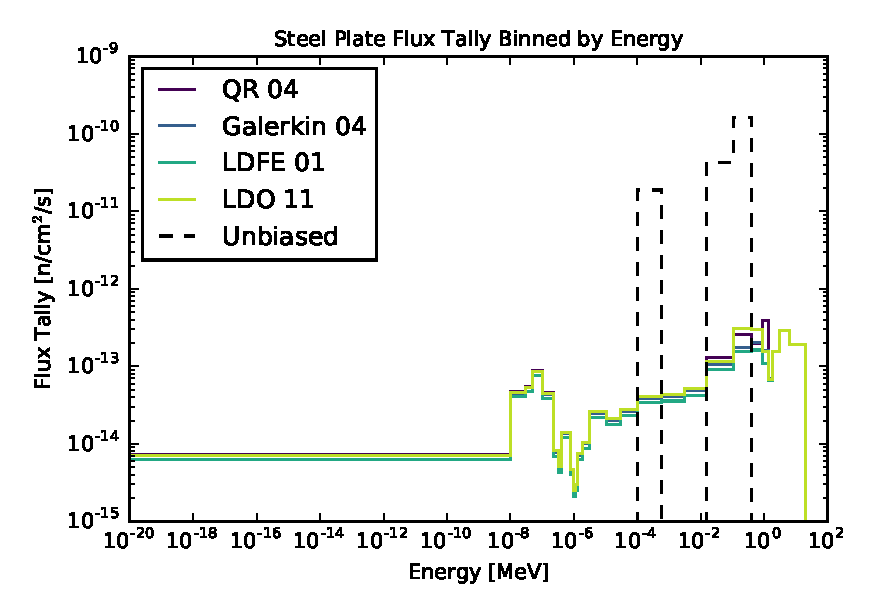
\includegraphics[max height=0.445\textheight]{img/steel-plots/mcnp/ebin-hist.eps}
\caption{Steel plate detector tally broken down by energy bin.}
\label{steel-tally-bin}
\end{figure}

\noindent This phenomenon has been 
previously documented \cite{wilsonslaybaugh} and can be largely attributed to the 
resonances in the iron cross section, shown in Figure \ref{fe-xs} with the 27n19g 
library energy group boundaries overlaid. The unresolved resonance region in the iron
cross section spans multiple energy groups, leading to inaccuracies in the discretized
multigroup cross section values used in deterministic calculations. To put this
directly in the context of the test case scenario at hand, Figure \ref{hist-xs} shows
the detector tally broken down by energy bin overlaid on the iron total cross section.
Unsurprisingly, the energy regions of large discrepancy are those in which the iron
cross section resonances lie.

\begin{figure}[!htb]
\centering
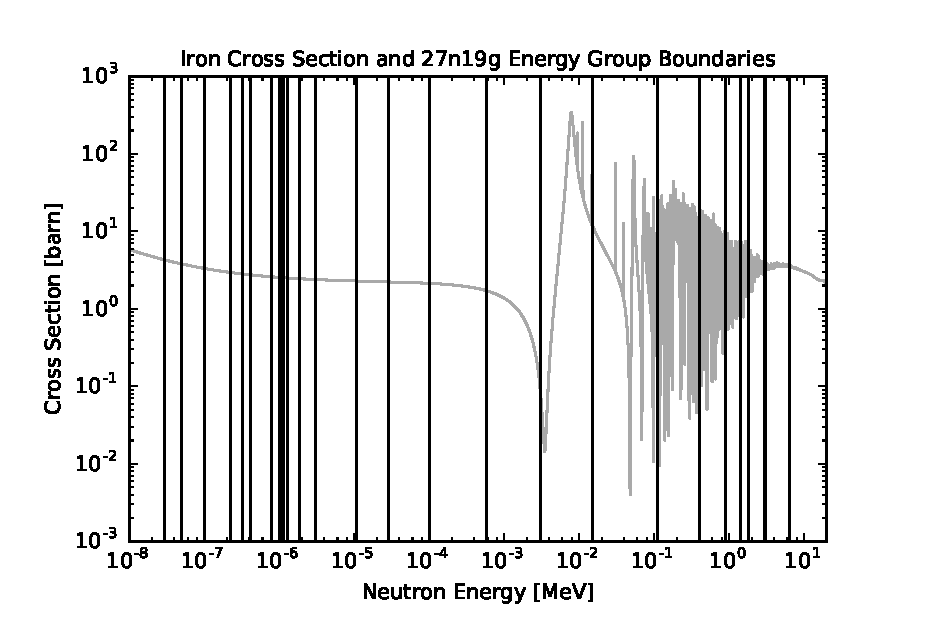
\includegraphics[max height=0.445\textheight]{img/steel-plots/fe-xs.eps}
\caption{ENDF iron total reaction cross section with 27n19g energy group limits 
         \cite{endf, advantg}.}
\label{fe-xs}
\end{figure}

\begin{figure}[!hbt]
\centering
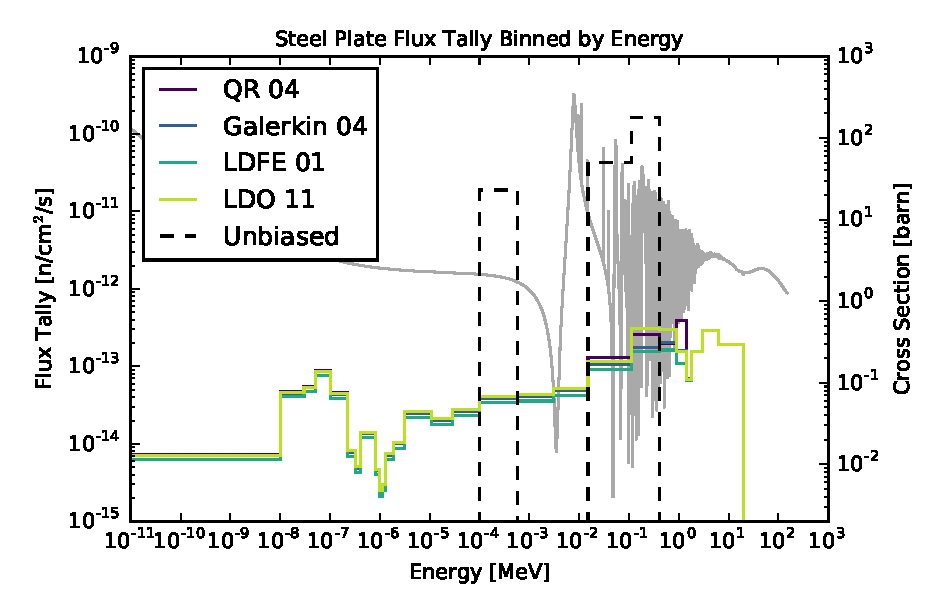
\includegraphics[max height=0.445\textheight]{img/steel-plots/mcnp/ebin-hist-xs.eps}
\caption{Steel plate detector tally broken down by energy bin with iron cross 
         section.}
\label{hist-xs}
\end{figure}

\FloatBarrier
Having explored the discrepancy between the biased and unbiased tally
results, we move on to looking at the Figures of Merit for the various Monte Carlo 
run results. Figure \ref{steel-cad-fom} shows the reported FOM value for the detector
tally for the various quadrature sets and orders. We again plot the results as a
function of angular mesh refinement with a black horizontal line denoting the FOM for
the unbiased Monte Carlo calculation. The biasing parameters corresponding to the 
LDFE quadrature set of order 1 result in the highest FOM value while those of the QR
set of order 1 result in the lowest FOM value. For all LDO quadrature sets of order 8
and above, the Figures of Merit are one order of magnitude greater than that of the
unbiased calculation.

\begin{figure}[!htb]
\centering
\includegraphics[max height=0.445\textheight]{img/steel-plots/mcnp/cadis-fom-4.eps}
\caption{FOM values for MCNP flux tally at the end of the steel plate.}
\label{steel-cad-fom}
\end{figure}

To conclude this section, we consider the overall trends in angular mesh refinement
in Figures \ref{steel-cad-tally} and \ref{steel-cad-fom}. It appears that the angular
mesh refinement does not have a great impact on the flux tally value in this scenario,
as all of the biased tally results fall within the same order of magnitude and do not
exhibit any trends as a function of the number of discrete angles used. The Figures 
of Merit vary somewhat more greatly. Specifically, the LDO biasing parameters appear
to gather around FOM values of 0.005 even as the number of discrete angles used 
is increased. So, for the steel plate in water detector tally in the context of the 
CADIS method, one could use a relatively low-order (i.e., order 8) LDO quadrature set 
to generate Monte Carlo biasing parameters that result in a Figure of Merit comparable to
(and better than most of, as seen here) those produced by finer angular meshes.

\FloatBarrier
\subsection{DLVN}

To study the DLVN problem in the context of the CADIS method, the adjoint source
was set to be the tally located at detector \#14 in the original experiment.
All of the adjoint scalar flux solutions shown in Figure \ref{dlvn-cad-adj-slices}
reflect this; the adjoint flux is highest at the specified detector location. The
differences in the adjoint scalar flux solutions shown in Figure 
\ref{dlvn-cad-adj-diff-rel} appear as ray effects from the relatively localized source
at the detector location as well as in the streaming pathway in the dog-legged void
section. Table \ref{dlvn-cad-diff-table} lists the extremal and average values of the 
relative differences between the LDO and standard quadrature results. Comparisons
between the Galerkin and LDFE quadrature sets versus the QR set are also given for
reference. On average, the LDO adjoint flux solution agrees best with the QR adjoint
flux solution with a difference of approximately 3.8\%.

\begin{table}[!hbt]
\centering
\caption{DLVN CADIS adjoint scalar flux extremal and average relative 
         differences.}
\label{dlvn-cad-diff-table}
\begin{tabular}{l|ccc}
\textbf{Comparison} & \textbf{Min. Diff.} & \textbf{Max. Diff.} & \textbf{Avg. Diff.} 
\\ \hline
LDO/QR              & 1\E{-5}             & 1.24\E{0}         & 3.78\E{-2} 
\rule{0pt}{2.6ex}   \\ 
LDO/Galerkin        & 3\E{-4}             & 5.01\E{0}         & 3.56\E{-1}          \\
LDO/LDFE            & 2\E{-5}             & 9.67\E{-1}        & 6.04\E{-2}          \\
Galerkin/QR         & 6\E{-1}             & 7.62\E{-1}        & 2.00\E{-1}          \\
LDFE/QR             & 2\E{-5}             & 3.07\E{-1}        & 5.31\E{-2}
\end{tabular}
\end{table}

\begin{figure}[!htb]
\centering
\begin{subfigure}{0.4\textwidth}
\includegraphics[max height=0.445\textheight]
{img/dlvn-plots/cad-adj/flux-qr04-slice.eps}
\subcaption{QR adjoint flux slice.}
\end{subfigure} ~
\begin{subfigure}{0.4\textwidth}
\includegraphics[max height=0.445\textheight]
{img/dlvn-plots/cad-adj/flux-gkn04-slice.eps}
\subcaption{Galerkin adjoint flux slice.}
\end{subfigure}
\\
\begin{subfigure}{0.4\textwidth}
\includegraphics[max height=0.445\textheight]
{img/dlvn-plots/cad-adj/flux-ldfe01-slice.eps}
\subcaption{LDFE adjoint flux slice.}
\end{subfigure} ~
\begin{subfigure}{0.4\textwidth}
\includegraphics[max height=0.445\textheight]
{img/dlvn-plots/cad-adj/flux-ldo11-slice.eps}
\subcaption{LDO adjoint flux slice.}
\end{subfigure}
\caption{DLVN adjoint scalar flux slices for the CADIS method.}
\label{dlvn-cad-adj-slices}
\end{figure}

\begin{figure}[!htb]
\centering
\begin{subfigure}{0.4\textwidth}
\includegraphics[max height=0.445\textheight]
{img/dlvn-plots/cad-adj/flux-diff-rel-qr04.eps}
\subcaption{LDO/QR flux rel. diff.}
\end{subfigure} ~
\begin{subfigure}{0.4\textwidth}
\includegraphics[max height=0.445\textheight]
{img/dlvn-plots/cad-adj/flux-diff-rel-gkn04.eps}
\subcaption{LDO/Galerkin flux rel. diff.}
\end{subfigure}
\\
\begin{subfigure}{0.4\textwidth}
\includegraphics[max height=0.445\textheight]
{img/dlvn-plots/cad-adj/flux-diff-rel-ldfe01.eps}
\subcaption{LDO/LDFE flux rel. diff.}
\end{subfigure}
\caption{DLVN adjoint scalar flux relative difference slices for the CADIS method.}
\label{dlvn-cad-adj-diff-rel}
\end{figure}

\clearpage
Moving forward, we look at the Monte Carlo results. For the DLVN case, 1\E{10}
neutron histories were simulated. Since the CADIS method is for one
local adjoint source, which we have set to detector \#14 here, the discussion in this
section will focus on the results for this specific detector location. Figure
\ref{dlvn-cad-tally} shows the MCNP-reported tally for the forward scalar flux at the
location of detector \#14. Here we see that all of the biased calculation values fall
within the error of the unbiased result. However, all of these tally calculations 
(biased and unbiased) do not match the experimentally calculated flux value of 
2.74\E{-7} $\pm$ 5\% n/cm$^2$/s at detector \#14.

\begin{figure}[!htb]
\centering
\includegraphics[max height=0.445\textheight]{img/dlvn-plots/mcnp/cadis-tally-14.eps}
\caption{Flux tally at detector \#14 in the DLVN problem with the CADIS method.}
\label{dlvn-cad-tally}
\end{figure}

\begin{figure}[!htb]
\centering
\includegraphics[max height=0.445\textheight]{img/dlvn-plots/mcnp/cadis-fom-14.eps}
\caption{FOM values for the DLVN problem detector \#14 tally with the CADIS 
         method.}
\label{dlvn-cad-fom}
\end{figure}

Figures \ref{dlvn-cad-tally} and \ref{dlvn-cad-fom} show similar convergence behavior 
with respect to angular mesh refinement for the biased tally calculations and Figure 
of Merit values. Beyond the lowest-order angular mesh refinement for each
quadrature type studied here, the tally result for this detector location using the
CADIS method is not impacted by further refining the angular mesh. The Figures of
Merit for the tally calculations reach a similar upper bound, but this happens more
slowly with respect to angular mesh refinement for the LDO quadrature sets. Like the
tally in the steel plate case above, the LDO quadrature set of order 8 is the optimal
choice with respect to flux tally result and FOM value for detector \#14 in the DLVN
experimental benchmark problem in the CADIS context.

\FloatBarrier
\subsection{Ispra Sodium Benchmark}
\label{sec:eurac-cad}

For these CADIS calculations, the adjoint source was set to be the detector
location farthest from the experimental neutron source. As with the previous cases, we will 
first examine the adjoint scalar flux solutions and then move on to the Monte Carlo results.
The representative LDO quadrature set used in the deterministic calculations
here is of order 9 with only 100 total angles and is
coarser than the other representative quadrature sets.

The adjoint scalar flux solutions are shown in Figure \ref{eurac-cad-slices} with
relative differences plotted in Figure \ref{eurac-cad-diff-rel} and listed in Table
\ref{eurac-cad-diff-table}. Since this
source is relatively localized in the overall problem scale, ray effects are seen in
the adjoint flux solutions as well as in the relative difference plots. For this case,
the Galerkin adjoint scalar flux matches most closely with the QR adjoint scalar flux;
a finer LDO angular mesh would likely show better agreement.

\begin{table}[!hbt]
\centering
\small
\caption{Ispra sodium test CADIS adjoint flux extremal and average relative 
         differences.}
\label{eurac-cad-diff-table}
\begin{tabular}{l|ccc}
\textbf{Comparison} & \textbf{Min. Diff.} & \textbf{Max. Diff.} & \textbf{Avg. Diff.} 
\\ \hline
LDO/QR              & 1\E{-8}             & 1.46\E{2}   & 9.71\E{-1}
\rule{0pt}{2.6ex}   \\ 
LDO/Galerkin        & 2\E{-5}             & 2.52\E{5}   & 5.74\E{2}  \\
LDO/LDFE            & 1\E{-6}             & 3.32\E{2}   & 1.28\E{0}  \\
Galerkin/QR         & 5\E{-6}             & 1.00\E{0}   & 4.62\E{-1} \\
LDFE/QR             & 6\E{-7}             & 8.10\E{1}   & 1.19\E{0}
\end{tabular}
\end{table}

\clearpage
\begin{figure}[!htb]
\begin{subfigure}{\textwidth}
\centering
\includegraphics[max height=0.445\textheight]
{img/eurac-plots/cad-adj/flux-qr04-slice.eps}
\subcaption{QR adjoint flux slice.}
\end{subfigure}
\\
\begin{subfigure}{\textwidth}
\centering
\includegraphics[max height=0.445\textheight]
{img/eurac-plots/cad-adj/flux-gkn04-slice.eps}
\subcaption{Galerkin adjoint flux slice.}
\end{subfigure}
\end{figure}
\clearpage
\begin{figure}[!htb]
\ContinuedFloat
\begin{subfigure}{\textwidth}
\centering
\includegraphics[max height=0.445\textheight]
{img/eurac-plots/cad-adj/flux-ldfe01-slice.eps}
\subcaption{LDFE adjoint flux slice.}
\end{subfigure}
\\
\begin{subfigure}{\textwidth}
\centering
\includegraphics[max height=0.445\textheight]
{img/eurac-plots/cad-adj/flux-ldo09-slice.eps}
\subcaption{LDO adjoint flux slice.}
\end{subfigure}
\caption{Ispra sodium adjoint scalar flux slices for the CADIS method.}
\label{eurac-cad-slices}
\end{figure}

\clearpage
\begin{figure}[!htb]
\begin{subfigure}{\textwidth}
\centering
\includegraphics[max height=0.445\textheight]
{img/eurac-plots/cad-adj/flux-diff-rel-qr04.eps}
\subcaption{LDO/QR flux relative difference.}
\end{subfigure}
\\
\begin{subfigure}{\textwidth}
\centering
\includegraphics[max height=0.445\textheight]
{img/eurac-plots/cad-adj/flux-diff-rel-gkn04.eps}
\subcaption{LDO/Galerkin flux relative difference.}
\end{subfigure}
\end{figure}
\clearpage
\begin{figure}[!htb]
\ContinuedFloat
\begin{subfigure}{\textwidth}
\centering
\includegraphics[max height=0.445\textheight]
{img/eurac-plots/cad-adj/flux-diff-rel-ldfe01.eps}
\subcaption{LDO/LDFE flux relative difference.}
\end{subfigure}
\caption{Ispra sodium adjoint scalar flux relative difference slices for the CADIS 
         method.}
\label{eurac-cad-diff-rel}
\end{figure}

Again, we will focus the analysis here on
the Monte Carlo results for the detector location set to be the adjoint source in the
CADIS context. Here, 1\E{9} neutron histories were simulated. 
Figure \ref{eurac-cad-tally} shows the calculated activity values for
the far detector location as a function of angular mesh refinement. All activity
values were calculated using the forward scalar flux reported by MCNP in combination
with Equation \ref{eq:act} and the data listed in Section \ref{sec:eurac-fwd}. All of
the biased results fall well within the statistical error of the unbiased calculation,
but the calculations are all four orders of magnitude greater than the experimentally
calculated activity of 0.00199 Bq/g listed in Table \ref{eurac-fwd-det}. One likely
reason for this is that the MCNP flux tallies used in these calculations include neutrons of 
all incident energies and not only those above the threshold for the \ce{^{32}S}(n,p)\ce{^{32}P}
reaction measured experimentally.

\begin{figure}[!htb]
\centering
\includegraphics[max height=0.445\textheight]{img/eurac-plots/mcnp/cadis-tally-74.eps}
\caption{Ispra sodium calculated activity in the far detector with the CADIS method.}
\label{eurac-cad-tally}
\end{figure}

\begin{figure}[!htb]
\centering
\includegraphics[max height=0.445\textheight]{img/eurac-plots/mcnp/cadis-fom-74.eps}
\caption{Ispra sodium far detector flux tally FOM values with the CADIS method.}
\label{eurac-cad-fom}
\end{figure}

Figure \ref{eurac-cad-tally} exhibits no trend for the calculated activity with
respect to angular mesh refinement; the coarsest angular mesh of each quadrature type
studied here is sufficient to achieve the same forward flux tally and calculated
activity value. The FOM values plotted in Figure \ref{eurac-cad-fom} show
differing trends for the different quadrature types. The QR biasing parameters tend
toward a Figure of Merit of approximately 1000, with the exception of those from the
quadrature set of order 4. Of the LDO quadrature sets tested here, the best
performance comes from the coarsest angular mesh, with the finest angular mesh not far
behind. So, for the Ispra sodium benchmark case in the CADIS method context, the LDO
quadrature set of order 3 would be the best one to use (of the LDO quadrature sets).

\FloatBarrier
\subsection{Simplified Portal Monitor}

To study calculations for the simplified portal monitor scenario in the context of the CADIS 
method, the adjoint source was set to be the top detector in the small array. The adjoint scalar
flux solutions are plotted in Figure \ref{cargo-cad-adj-slices}. Ray effects appear
drastically in all of the adjoint scalar flux solutions. Figure \ref{cargo-cad-gkn}
shows regions where the adjoint scalar flux solution is negative for the 
representative Galerkin quadrature set; these regions are plotted in white.
Because of these negative flux regions, Table \ref{cargo-cad-diff-table} shows the 
extremal values of the magnitudes of the relative flux differences, calculated as

\begin{equation}
\phi_{\mathrm{diff}} = 
\frac{\left|\phi_{\mathrm{LDO}}-\phi_{\mathrm{ref}}\right|}{\left|\phi_{\mathrm{ref}}\right|}.
\label{flux-diff-gkn}
\end{equation}

\noindent All of the flux solutions show poor agreement, likely because of the localized source
and streaming paths created by this scenario's materials and geometry. Still, the LDO adjoint
scalar flux solution agrees with the QR adjoint scalar flux solution better than the Galerkin
or LDFE solutions, on average.

\begin{table}[!hbt]
\centering
\caption{Portal monitor CADIS adjoint scalar flux extremal and average relative 
         differences.}
\label{cargo-cad-diff-table}
\begin{tabular}{l|ccc}
\textbf{Comparison} & \textbf{Min. Diff.} & \textbf{Max. Diff.} & \textbf{Avg. Diff.} 
\\ \hline
LDO/QR              & 2\E{-4}             & 1.83\E{2}    & 2.27\E{0}
\rule{0pt}{2.6ex}   \\ 
LDO/Galerkin        & 1\E{-4}             & 6.20\E{4}    & 4.29\E{1}  \\
LDO/LDFE            & 2\E{-4}             & 2.54\E{2}    & 3.46\E{0}   \\
Galerkin/QR         & 1\E{-3}             & 2.59\E{2}    & 3.81\E{0}   \\
LDFE/QR             & 6\E{-5}             & 6.48\E{1}    & 2.21\E{0}
\end{tabular}
\end{table}

\clearpage
\begin{figure}[!htb]
\begin{subfigure}{\textwidth}
\centering
\includegraphics[max height=0.445\textheight]
{img/cargo-plots/cad-adj/flux-qr04-slice.eps}
\subcaption{QR adjoint flux slice.}
\end{subfigure}
\\
\begin{subfigure}{\textwidth}
\centering
\includegraphics[max height=0.445\textheight]
{img/cargo-plots/cad-adj/flux-gkn04-slice.eps}
\subcaption{Galerkin adjoint flux slice.}
\label{cargo-cad-gkn}
\end{subfigure}
\end{figure}
\clearpage
\begin{figure}[!htb]
\ContinuedFloat
\begin{subfigure}{\textwidth}
\centering
\includegraphics[max height=0.445\textheight]
{img/cargo-plots/cad-adj/flux-ldfe01-slice.eps}
\subcaption{LDFE adjoint flux slice.}
\end{subfigure}
\\
\begin{subfigure}{\textwidth}
\centering
\includegraphics[max height=0.445\textheight]
{img/cargo-plots/cad-adj/flux-ldo11-slice.eps}
\subcaption{LDO adjoint flux slice.}
\end{subfigure}
\caption{Simplified portal monitor adjoint scalar flux slices for the CADIS method.}
\label{cargo-cad-adj-slices}
\end{figure}

\clearpage
\begin{figure}[!htb]
\begin{subfigure}{\textwidth}
\centering
\includegraphics[max height=0.445\textheight]
{img/cargo-plots/cad-adj/flux-diff-rel-qr04.eps}
\subcaption{LDO/QR flux relative difference.}
\end{subfigure}
\\
\begin{subfigure}{\textwidth}
\centering
\includegraphics[max height=0.445\textheight]
{img/cargo-plots/cad-adj/flux-diff-rel-gkn04.eps}
\subcaption{LDO/Galerkin flux relative difference.}
\end{subfigure}
\end{figure}
\clearpage
\begin{figure}[!htb]
\ContinuedFloat
\begin{subfigure}{\textwidth}
\centering
\includegraphics[max height=0.445\textheight]
{img/cargo-plots/cad-adj/flux-diff-rel-ldfe01.eps}
\subcaption{LDO/LDFE flux relative difference.}
\end{subfigure}
\caption{Portal monitor adjoint scalar flux relative difference slices for the CADIS 
         method.}
\label{cargo-cad-adj-diff-rel}
\end{figure}

Finally, we move on to the results and analysis of the Monte Carlo calculations, in which
1\E{9} particle histories were simulated.
Again, since the CADIS adjoint source was set to be the top detector location, we
focus the discussion in this section on the results for that specific location.
Figures \ref{cargo-cad-tally} and \ref{cargo-cad-fom} show the MCNP-reported forward scalar 
flux tally values and Figures of Merit, respectively. As with the other test cases, the
values are plotted as a function of the number of quadrature points used to generate
the biasing parameters in order to explore the impact of angular mesh refinement on
flux tally and FOM.

\begin{figure}[!htb]
\centering
\includegraphics[max height=0.445\textheight]{img/cargo-plots/mcnp/cadis-tally-14.eps}
\caption{Flux tally in the portal monitor top detector using the CADIS method.}
\label{cargo-cad-tally}
\end{figure}

\begin{figure}[!htb]
\centering
\includegraphics[max height=0.445\textheight]{img/cargo-plots/mcnp/cadis-fom-14.eps}
\caption{CADIS method FOM values for the portal monitor top detector flux tally.}
\label{cargo-cad-fom}
\end{figure}

Similar to other test cases, the flux tally values reported in Figure 
\ref{cargo-cad-tally} show a trend of converging to a stable value after the first few
coarsest angular meshes. The flux tally values from the biased calculations all fall
within the statistical error of that of the unbiased calculation but appear to require
a minimum value of approximately 100 discrete angular values in order to stabilize.
Figure \ref{cargo-cad-fom} shows a strong correlation between the number of quadrature
points and the flux tally FOM, eventually approaching an upper limit around 100.
The LDO Figures of Merit increase most rapidly with the
number of quadrature points used, so one would want to use a higher-order LDO 
quadrature set to generate Monte Carlo biasing parameters.

\FloatBarrier
\subsection{Summary}

In this section, we examined the deterministic and Monte Carlo results for the four
test case scenarios in the context of the CADIS method. 
For all of the test cases, little correlation was noted between angular mesh
refinement and MCNP-reported forward flux tally value beyond the suggestion to use
at least 100 discrete angles for the simplified portal monitor scenario. The reported
FOM values also exhibited minimal correlation with angular mesh refinement except in
the case of the portal monitor scenario, where the flux tally FOM increased with angular mesh
refinement while approaching an upper limit.

For the three test cases in which neutrons were transported, the LDO quadrature sets 
of lower orders (3 and 8) were the most effective of the LDO sets for both flux tally
value and FOM achievement. That is, if one were interested in using an LDO quadrature
set to generate Monte Carlo biasing parameters for a given neutron transport problem
in the context of the CADIS method, we would suggest performing the deterministic
calculation with an LDO quadrature set of order 8. For a photon transport problem
considered in the CADIS context, we would suggest the finest available LDO quadrature
set, based on the results seen here.

\FloatBarrier
\section{FW-CADIS Calculations}

Finally, we examine the performance of the various quadrature types in the context of
the \fwc\ method. Similar to the analysis for the CADIS method, we will first look at 
the deterministic adjoint scalar flux solutions from the representative quadrature 
sets to compare the calculations using the LDO equations versus the standard 
quadrature types. Recalling Section \ref{sec:fwcadis}, the \fwc\ method incorporates 
both forward and adjoint scalar flux solutions. Because the adjoint source may be
specified differently between the CADIS and \fwc\ methods, it is instructive to look
at the \fwc\ deterministic adjoint scalar flux solutions. However, the deterministic
forward flux solutions used in the \fwc\ method are the same as those discussed
in Section \ref{sec:det-fwd} and so we will not repeat the analysis here. Lastly, we
again look at result metrics from the various Monte Carlo runs to compare the variance
reduction parameter generation efficacy of the different quadrature types.

\subsection{Steel Plate in Water}

For the \fwc\ calculations for the steel plate in water, the adjoint source was set to
be a mesh tally over all of the air beyond the steel plate. The discretization for the
adjoint source mesh tally is the same as that listed in 
Section \ref{sec:steel_params}. Specifically, the adjoint source mesh is identical to
the overall problem mesh in the $x-$ and $y-$directions but starts at $z = 130$ cm and
extends to the problem boundary at $z = 140$ cm.

Figure \ref{steel-fwc-adj-slices} shows the adjoint scalar flux solutions for the
representative quadrature sets for the steel plate embedded in water. As expected, in
each solution, the adjoint flux is highest in the chosen adjoint source region for the
problem and decreases logarithmically in the $z-$direction. Table 
\ref{steel-fwc-diff-table} lists the minimum, maximum, and average relative adjoint
scalar flux solution differences for the comparisons plotted in Figure 
\ref{steel-fwc-adj-diff-rel}. As with earlier cases, the Galerkin/QR and LDFE/QR
comparisons are also tabulated for reference. Like other deterministic flux
comparisons for the steel plate embedded in water, the LDO flux solution best matches
the QR flux solution, with an average relative difference of 4.6\% for the \fwc\ adjoint
scalar flux.

\begin{table}[!hbt]
\centering
\caption{Steel plate \fwc\ adjoint scalar flux extremal and average relative 
         differences.}
\label{steel-fwc-diff-table}
\begin{tabular}{l|ccc}
\textbf{Comparison} & \textbf{Min. Diff.} & \textbf{Max. Diff.} & \textbf{Avg. Diff.} 
\\ \hline
LDO/QR              & 2\E{-4}             & 1.66\E{-1}    & 4.63\E{-2}
\rule{0pt}{2.6ex}   \\ 
LDO/Galerkin        & 2\E{-5}             & 1.85\E{0}     & 7.16\E{-1}      \\
LDO/LDFE            & 8\E{-2}             & 2.41\E{-1}    & 1.92\E{-1}      \\
Galerkin/QR         & 5\E{-4}             & 5.98\E{0}     & 2.85\E{0}      \\
LDFE/QR             & 3\E{-2}             & 3.37\E{-1}    & 2.09\E{-1}
\end{tabular}
\end{table}

\noindent Comparing Figure \ref{steel-fwc-adj-diff-rel} with Figure 
\ref{steel-cad-adj-diff-rel}, we see that the relative differences among the \fwc\ adjoint
scalar flux solutions are more uniform than those of the CADIS adjoint flux solutions. This is
to be expected, as the CADIS adjoint source is much more localized than the \fwc\ for the
steel plate scenario studies conducted here.

\begin{figure}[!htb]
\centering
\begin{subfigure}{0.4\textwidth}
\includegraphics[max height=0.445\textheight]
{img/steel-plots/fwc-adj/flux-qr04-slice.eps}
\subcaption{QR adjoint flux slice.}
\end{subfigure} ~
\begin{subfigure}{0.4\textwidth}
\includegraphics[max height=0.445\textheight]
{img/steel-plots/fwc-adj/flux-gkn04-slice.eps}
\subcaption{Galerkin adjoint flux slice.}
\end{subfigure}
\\
\begin{subfigure}{0.4\textwidth}
\includegraphics[max height=0.445\textheight]
{img/steel-plots/fwc-adj/flux-ldfe01-slice.eps}
\subcaption{LDFE adjoint flux slice.}
\end{subfigure} ~
\begin{subfigure}{0.4\textwidth}
\includegraphics[max height=0.445\textheight]
{img/steel-plots/fwc-adj/flux-ldo11-slice.eps}
\subcaption{LDO adjoint flux slice.}
\end{subfigure}
\caption{Steel plate adjoint scalar flux slices for the \fwc\ method.}
\label{steel-fwc-adj-slices}
\end{figure}

\begin{figure}[!htb]
\centering
\begin{subfigure}{0.4\textwidth}
\includegraphics[max height=0.445\textheight]
{img/steel-plots/fwc-adj/flux-diff-rel-qr04.eps}
\subcaption{LDO/QR flux rel. diff.}
\end{subfigure} ~
\begin{subfigure}{0.4\textwidth}
\includegraphics[max height=0.445\textheight]
{img/steel-plots/fwc-adj/flux-diff-rel-gkn04.eps}
\subcaption{LDO/Galerkin flux rel. diff.}
\end{subfigure}
\\
\begin{subfigure}{0.4\textwidth}
\includegraphics[max height=0.445\textheight]
{img/steel-plots/fwc-adj/flux-diff-rel-ldfe01.eps}
\subcaption{LDO/LDFE flux rel. diff.}
\end{subfigure}
\caption{Steel plate adjoint flux relative difference slices for the \fwc\
         method.}
\label{steel-fwc-adj-diff-rel}
\end{figure}

\clearpage
Next, we will look at the results for the mesh tally in the air region of the 
scenario. The Monte Carlo run with biasing parameters from the Galerkin quadrature 
set of order 2 was not able to finish in a timely manner for the hardware
configuration used in this work, so Monte Carlo results for this data point are not
included here. The calculations for this test case scenario used 1\E{9} neutron histories.

Figure \ref{steel-fwc-tally} shows the total tally summed over all air in the
problem for the biased and unbiased calculations. The biased calculations are plotted
as a function of angular mesh refinement and the unbiased calculation value is shown
as a black horizontal line. Like the CADIS method, the \fwc\ method generates biasing
parameters such that the biased Monte Carlo flux tally results all fall far below that
of the unbiased calculation. Similarly, in this case, the angular mesh refinement has
little impact on the tally result. So, if using an LDO quadrature set to generate
biasing parameters with the \fwc\ method in a similar scenario, a low-order LDO
angular mesh could be used to good effect.

\begin{figure}[!htb]
\centering
\includegraphics[max height=0.445\textheight]{img/steel-plots/mcnp/fwc-tally.eps}
\caption{Flux tally over the air region in the steel plate test with the \fwc\ method.}
\label{steel-fwc-tally}
\end{figure}

To analyze the performance of the representative quadrature sets' variance reduction
parameters for the steel plate in water case using the \fwc\ method, we will look at
the average FOM values over the entire adjoint source mesh tally. The Figures of
Merit were calculated by taking the average relative error over all spatial cells in the
air block mesh tally and using that mean value in combination with the MCNP-reported 
computer time and Equation \ref{eq:fom}. Figure \ref{steel-fwc-fom} shows these
average Figures of Merit as a function of the number of angles used in generating the
biasing parameters. The average FOM for the unbiased calculation is shown as a
horizontal black line.

\begin{figure}[!htb]
\centering
\includegraphics[max height=0.445\textheight]{img/steel-plots/mcnp/fwcadis-fom.eps}
\caption{Average FOM values for the mesh tally in the \fwc\ steel plate scenario.}
\label{steel-fwc-fom}
\end{figure}

We see a different trend here in that the highest average FOM values tend to come from
quadrature sets with mid-range angular mesh refinement; the coarsest and finest
angular meshes produce Monte Carlo biasing parameters that result in reduced Figures
of Merit. Considering Figures \ref{steel-fwc-tally} and \ref{steel-fwc-fom}, we note
that one would wish to use a lower-order (e.g., order 5) LDO quadrature set to generate
variance reduction parameters for a Monte Carlo mesh tally using the \fwc\ method.

\FloatBarrier
\subsection{DLVN}

Considering the DLVN case with the \fwc\ method, the adjoint source was specified to
be the combination of all of the detector locations in the problem. In accordance 
with this, the adjoint scalar flux solutions shown in Figure \ref{dlvn-fwc-adj-slices}
demonstrate the highest source values in the region where four out of the six
detector locations are concentrated. Figure \ref{dlvn-fwc-adj-diff-rel} displays the
relative differences between the LDO adjoint scalar flux solution and those of
the three standard quadrature types with extremal and average relative difference
values listed in Table \ref{dlvn-fwc-diff-table}. 
Of the standard quadrature types, the LDO adjoint flux solution differs the least from the QR
adjoint flux solution, with an average relative difference of about 11\% for this \fwc\ adjoint
source specification for the DLVN problem. Given the more spatially 
generalized source specification, it is unsurprising to see uniform differences in 
Figures \ref{dlvn-fwc-qr-ldo} and \ref{dlvn-fwc-ldfe-ldo}. The nonuniform differences 
in Figure \ref{dlvn-fwc-gkn-ldo} may be attributed to the relative coarseness of the
representative Galerkin quadrature set.

\begin{table}[!hbt]
\centering
\caption{DLVN \fwc\ adjoint scalar flux extremal and average relative differences.}
\label{dlvn-fwc-diff-table}
\begin{tabular}{l|ccc}
\textbf{Comparison} & \textbf{Min. Diff.} & \textbf{Max. Diff.} & \textbf{Avg. Diff.} 
\\ \hline
LDO/QR              & 1\E{-3}             & 4.32\E{-1} & 1.12\E{-1}
\rule{0pt}{2.6ex}   \\ 
LDO/Galerkin        & 2\E{-5}             & 1.90\E{0}  & 1.79\E{-1}      \\
LDO/LDFE            & 1\E{-2}             & 3.97\E{-1} & 1.73\E{-1}      \\
Galerkin/QR         & 2\E{-4}             & 6.88\E{-1} & 2.68\E{-1}      \\
LDFE/QR             & 4\E{-4}             & 2.58\E{-1} & 5.42\E{-2}
\end{tabular}
\end{table}

\begin{figure}[!htb]
\centering
\begin{subfigure}{0.4\textwidth}
\includegraphics[max height=0.445\textheight]
{img/dlvn-plots/fwc-adj/flux-qr04-slice.eps}
\subcaption{QR adjoint flux slice.}
\end{subfigure} ~
\begin{subfigure}{0.4\textwidth}
\includegraphics[max height=0.445\textheight]
{img/dlvn-plots/fwc-adj/flux-gkn04-slice.eps}
\subcaption{Galerkin adjoint flux slice.}
\end{subfigure}
\\
\begin{subfigure}{0.4\textwidth}
\includegraphics[max height=0.445\textheight]
{img/dlvn-plots/fwc-adj/flux-ldfe01-slice.eps}
\subcaption{LDFE adjoint flux slice.}
\end{subfigure} ~
\begin{subfigure}{0.4\textwidth}
\includegraphics[max height=0.445\textheight]
{img/dlvn-plots/fwc-adj/flux-ldo11-slice.eps}
\subcaption{LDO adjoint flux slice.}
\end{subfigure}
\caption{DLVN adjoint scalar flux slices for the \fwc\ method.}
\label{dlvn-fwc-adj-slices}
\end{figure}

\begin{figure}[!htb]
\centering
\begin{subfigure}{0.4\textwidth}
\includegraphics[max height=0.445\textheight]
{img/dlvn-plots/fwc-adj/flux-diff-rel-qr04.eps}
\subcaption{LDO/QR flux rel. diff.}
\label{dlvn-fwc-qr-ldo}
\end{subfigure} ~
\begin{subfigure}{0.4\textwidth}
\includegraphics[max height=0.445\textheight]
{img/dlvn-plots/fwc-adj/flux-diff-rel-gkn04.eps}
\subcaption{LDO/Galerkin flux rel. diff.}
\label{dlvn-fwc-gkn-ldo}
\end{subfigure}
\\
\begin{subfigure}{0.4\textwidth}
\includegraphics[max height=0.445\textheight]
{img/dlvn-plots/fwc-adj/flux-diff-rel-ldfe01.eps}
\subcaption{LDO/LDFE flux rel. diff.}
\label{dlvn-fwc-ldfe-ldo}
\end{subfigure}
\caption{DLVN adjoint scalar flux relative difference slices for the \fwc\ method.}
\label{dlvn-fwc-adj-diff-rel}
\end{figure}

\clearpage
Moving on to the Monte Carlo results and analysis, we look at the flux tallies and 
Figures of Merit for all of the detector locations in the DLVN experimental benchmark.
Recall that 1\E{10} particle histories were simulated.
Figure \ref{dlvn-fwc-tally} shows all of the detector locations' MCNP-reported forward scalar
flux tallies plotted as a function of angular mesh refinement used to generate biasing 
parameters in addition to the Figures of Merit for the flux tallies.
In each plot, the unbiased flux tally result is shown as a horizontal black line.

Figures \ref{dlvn-fwc-5} and \ref{dlvn-fwc-9} exhibit the same lack of trend in flux tally as a
function of angular mesh refinement. That is, in general, for detector locations \#5 and \#9,
using more discrete angles in the \fwc\ deterministic calculations does not greatly impact the
flux tally result from MCNP. Figures \ref{dlvn-fwc-13} and \ref{dlvn-fwc-14} show similar
behavior with the exception of the most coarse angular meshes. For these detector locations, any
angular mesh refinement other than the coarsest angular mesh will produce a consistent forward 
scalar flux tally result. Figures \ref{dlvn-fwc-11} and \ref{dlvn-fwc-12} show slightly more
variation in flux tally result with angular mesh refinement. These two detector locations' 
tallies have also higher statistical error relative to those at the other detector locations. 
Overall, though, the flux tallies at detectors \#11 and \#12 are not heavily impacted by the
refinement of the angular mesh used in generating the Monte Carlo biasing parameters, but
a mid-range number of quadrature points should be used to avoid the large statistical
errors seen at the extreme ends of the angular mesh refinement spectrum.

Like their corresponding flux tally graphs, Figures \ref{dlvn-fwc-5}, \ref{dlvn-fwc-9}, and
\ref{dlvn-fwc-13} show almost no variation in FOM with angular mesh refinement for the tallies
at detector locations \#5, \#9, and \#13. This is to be expected, considering the uniform
statistical error and stable flux tally results at these locations. Figure \ref{dlvn-fwc-11}
shows variation in FOM with angular mesh refinement that is more varied, which corresponds to
the larger statistical uncertainties in the flux tally values for detector \#11. Figure
\ref{dlvn-fwc-12} shows little variation in FOM with angular mesh refinement with the 
exception of the finest QR set. Lastly, \ref{dlvn-fwc-14} shows an upper FOM limit of 
approximately 200 across all quadrature types, with the Figure of Merit largely consistent
across quadrature types with the exception of QR angular meshes.

In Table \ref{dlvn-fwc-det} we compare the Monte Carlo forward flux tally results for the 
representative quadrature sets listed in Section \ref{params}. Results from the unbiased Monte 
Carlo calculation are also included for comparison. All Monte Carlo
flux tally values are reported with an uncertainty of one standard deviation. For all detector
locations, the Monte Carlo flux tallies do not match the experimentally measured flux values for
any of the representative quadrature sets or the unbiased calculation, so we only compare the
Monte Carlo calculations in this table. We do note that the Monte Carlo calculations
overestimate the flux tally at all detector locations with the exception of detector \#13.
The flux tallies at detectors 5, 9, 13, and 14 all match within statistical uncertainty for all
of the Monte Carlo calculations. At detector \#11, the biased Monte Carlo calculations match
within standard error, but the calculations using the QR and LDO biasing parameter fall outside
of the error bounds of the unbiased calculation. Somewhat similarly, at detector \#14, all of
the biased calculations match one another within statistical uncertainty, but they are all
outside of the error bounds of the unbiased flux tally calculation.

\begin{table}[!htb]
\centering
\footnotesize
\caption{DLVN benchmark flux tallies [n/cm$^2$/s] calculated with \fwc.}
\label{dlvn-fwc-det}
\begin{tabular}{l|ccccc}
         & \textbf{QR} & \textbf{Galerkin} & \textbf{LDFE} 
         & \textbf{LDO} & \textbf{Unbiased}  \\ \hline
 Det. \#5 & \mr{1.3341 $\pm$ 0.0003} & \mr{1.3344 $\pm$ 0.0003} & \mr{1.3347 $\pm$ 0.0004} &
            \mr{1.3344 $\pm$ 0.0003} & \mr{1.3315 $\pm$ 0.0092} \rule{0pt}{2.6ex} \\
    (\E{-7})      &    &   &  &   &    \\
 Det. \#9 & \mr{2.5225 $\pm$ 0.0005} & \mr{2.5224 $\pm$ 0.0005} & \mr{2.5229 $\pm$ 0.0004} &
            \mr{2.2555 $\pm$ 0.0004} & \mr{2.5104 $\pm$ 0.0127} \rule{0pt}{2.6ex}  \\
   (\E{-7}) &   &  &  &  &   \\
 Det. \#11 & \mr{1.4420 $\pm$ 0.0005} & \mr{1.4451 $\pm$ 0.0027} & \mr{1.4446 $\pm$ 0.0026} &
            \mr{1.4463 $\pm$ 0.0015} & \mr{1.4463 $\pm$ 0.0010} \rule{0pt}{2.6ex} \\
   (\E{-5}) &   &  &  &  &   \\
 Det. \#12 & \mr{2.4749 $\pm$ 0.0004} & \mr{2.4743 $\pm$ 0.0004} & \mr{2.4751 $\pm$ 0.0004} &
            \mr{2.4744 $\pm$ 0.0004} & \mr{2.4684 $\pm$ 0.0042}  \rule{0pt}{2.6ex} \\
    (\E{-6}) &   &  &  &  &   \\
 Det. \#13 & \mr{4.3984 $\pm$ 0.0011} & \mr{4.3997 $\pm$ 0.0011} & \mr{4.3994 $\pm$ 0.0011} &
            \mr{4.3983 $\pm$ 0.0011} & \mr{4.4170 $\pm$ 0.0175}  \rule{0pt}{2.6ex} \\
    (\E{-7}) &   &  &  &  &   \\
 Det. \#14 & \mr{7.0070 $\pm$ 0.0025} & \mr{7.0829 $\pm$ 0.0045} & \mr{7.0813 $\pm$ 0.0026} &
            \mr{7.0834 $\pm$ 0.0032} & \mr{7.0694 $\pm$ 0.0216}  \rule{0pt}{2.6ex} \\
    (\E{-7}) &   &  &  &  &   \\ \hline
\end{tabular}
\end{table}

To examine the FOM values in a more quantifiable way, Table \ref{dlvn-fwc-fom-table} lists the
FOM values for all detector locations for each of the representative quadrature sets as well as
the unbiased calculation. The maximum FOM value at each detector location is emphasized.
Of the six detector locations, the LDO quadrature set achieves the highest FOM
for two of the locations. The QR quadrature set is the only other type to also
deliver the highest FOM for two out of six detectors; the Galerkin and LDFE
quadrature set biasing parameters each only achieve the highest FOM at one detector.
So, the LDO quadrature set's biasing parameters perform comparably
to those from the QR quadrature set with respect to obtaining high FOM values
for multiple detector locations using the \fwc\ method for the DLVN problem.

\begin{table}[!hbt]
\centering
\caption{\fwc\ FOM values for representative quadratures for the DLVN problem.}
\label{dlvn-fwc-fom-table}
\begin{tabular}{l|cccccc}
\multicolumn{1}{l|}{Quad. Type}
& \multicolumn{1}{l}{Det. \#5}
& \multicolumn{1}{l}{Det. \#9}
& \multicolumn{1}{l}{Det. \#11}
& \multicolumn{1}{l}{Det. \#12}
& \multicolumn{1}{l}{Det. \#13}
& \multicolumn{1}{l}{Det. \#14}
\\ \hline
\begin{tabular}[c]{@{}l@{}}   QR \end{tabular} 
& \begin{tabular}[c]{@{}c@{}} 483.01 \end{tabular} % fom for #5
& \begin{tabular}[c]{@{}c@{}} 709.51 \end{tabular} % fom for #9
& \begin{tabular}[c]{@{}c@{}} \textbf{202.66} \end{tabular} % fom for #11
& \begin{tabular}[c]{@{}c@{}} 747.91 \end{tabular} % fom for #12
& \begin{tabular}[c]{@{}c@{}} 380.84 \end{tabular} % fom for #13
& \begin{tabular}[c]{@{}c@{}} \textbf{185.40} \end{tabular} % fom for #14
\\
\begin{tabular}[c]{@{}l@{}}   Galerkin \end{tabular} 
& \begin{tabular}[c]{@{}c@{}} \textbf{527.79} \end{tabular} % fom for #5
& \begin{tabular}[c]{@{}c@{}} 649.88 \end{tabular} % fom for #9
& \begin{tabular}[c]{@{}c@{}} 5.9934 \end{tabular} % fom for #11
& \begin{tabular}[c]{@{}c@{}} 798.88 \end{tabular} % fom for #12
& \begin{tabular}[c]{@{}c@{}} 326.11 \end{tabular} % fom for #13
& \begin{tabular}[c]{@{}c@{}} 52.098 \end{tabular} % fom for #14
\\
\begin{tabular}[c]{@{}l@{}}   LDFE \end{tabular} 
& \begin{tabular}[c]{@{}c@{}} 310.28 \end{tabular} % fom for #5
& \begin{tabular}[c]{@{}c@{}} 710.43 \end{tabular} % fom for #9
& \begin{tabular}[c]{@{}c@{}} 6.6749 \end{tabular} % fom for #11
& \begin{tabular}[c]{@{}c@{}} 926.28 \end{tabular} % fom for #12
& \begin{tabular}[c]{@{}c@{}} \textbf{391.62} \end{tabular} % fom for #13
& \begin{tabular}[c]{@{}c@{}} 166.51 \end{tabular} % fom for #14
\\
\begin{tabular}[c]{@{}l@{}}   LDO \end{tabular}
& \begin{tabular}[c]{@{}c@{}} 478.24 \end{tabular} % fom for #5
& \begin{tabular}[c]{@{}c@{}} \textbf{721.22} \end{tabular} % fom for #9
& \begin{tabular}[c]{@{}c@{}} 19.959 \end{tabular} % fom for #11
& \begin{tabular}[c]{@{}c@{}} \textbf{943.96} \end{tabular} % fom for #12
& \begin{tabular}[c]{@{}c@{}} 369.42 \end{tabular} % fom for #13
& \begin{tabular}[c]{@{}c@{}} 110.40 \end{tabular} % fom for #14
\\
Unbiased  & 0.14912 & 0.27845 & 14.555 & 2.5256 & 0.45376 & 0.76362
\end{tabular}
\end{table}

In summary, for test case scenarios such as the DLVN problem in which the \fwc\ method is used
to generate Monte Carlo variance reduction parameters to optimize the response at multiple
flux tally detector locations, a relatively coarse quadrature set of any of the types studied
here can be used to sufficient effect. However, the coarsest available quadrature sets should
be avoided; flux tally results and Figures of Merit for the various detector locations tend to
level out as a function of angular mesh refinement beyond the quadrature sets with the fewest
number of angles. In particular, if using an LDO quadrature set in another similar scenario, we
would suggest using a point set of order 5 or 8.

\begin{figure}[!htb]
\begin{subfigure}{\linewidth}
\centering
\includegraphics[max height=0.445\textheight]
{img/dlvn-plots/mcnp/fwc-5.eps}
\subcaption{MCNP-reported forward flux tally and FOM values at detector \#5.}
\label{dlvn-fwc-5}
\end{subfigure} 
\\
\begin{subfigure}{\linewidth}
\centering
\includegraphics[max height=0.445\textheight]
{img/dlvn-plots/mcnp/fwc-9.eps}
\subcaption{MCNP-reported forward flux tally and FOM values at detector \#9.}
\label{dlvn-fwc-9}
\end{subfigure}
\end{figure}
\clearpage
\begin{figure}[!htb]
\ContinuedFloat
\begin{subfigure}{\linewidth}
\centering
\includegraphics[max height=0.445\textheight]
{img/dlvn-plots/mcnp/fwc-11.eps}
\subcaption{MCNP-reported forward flux tally and FOM values at detector \#11.}
\label{dlvn-fwc-11}
\end{subfigure}
\\
\begin{subfigure}{\linewidth}
\centering
\includegraphics[max height=0.445\textheight]
{img/dlvn-plots/mcnp/fwc-12.eps}
\subcaption{MCNP-reported forward flux tally and FOM values at detector \#12.}
\label{dlvn-fwc-12}
\end{subfigure}
\end{figure}
\clearpage
\begin{figure}[!htb]
\ContinuedFloat
\begin{subfigure}{\linewidth}
\centering
\includegraphics[max height=0.445\textheight]
{img/dlvn-plots/mcnp/fwc-13.eps}
\subcaption{MCNP-reported forward flux tally and FOM values at detector \#13.}
\label{dlvn-fwc-13}
\end{subfigure} 
\\
\begin{subfigure}{\linewidth}
\centering
\includegraphics[max height=0.445\textheight]
{img/dlvn-plots/mcnp/fwc-14.eps}
\subcaption{MCNP-reported forward flux tally and FOM values at detector \#14.}
\label{dlvn-fwc-14}
\end{subfigure}
\caption{\fwc\ flux tallies and FOM values for the DLVN problem.}
\label{dlvn-fwc-tally}
\end{figure}

\FloatBarrier
\subsection{Ispra Sodium Benchmark}

As in the previous case, the adjoint source for the Ispra sodium benchmark problem in
the context of the \fwc\ method was specified to be the combination of all of the 
detector locations in the problem. Figure \ref{eurac-fwc-slices} shows the adjoint scalar
flux solutions for the representative quadrature sets based on this specification. Relative
differences between the representative LDO adjoint scalar flux and the standard quadratures'
adjoint scalar fluxes are shown in Figure \ref{eurac-fwc-diff-rel} with minimum, maximum, and
average relative differences listed in Table \ref{eurac-fwc-diff-table}. Again, comparisons of
the QR flux solution against the Galerkin and LDFE flux solutions are tabulated for reference
as well.

\begin{table}[!hbt]
\centering
\caption{Ispra sodium \fwc\ adjoint flux extremal and average relative differences.}
\label{eurac-fwc-diff-table}
\begin{tabular}{l|ccc}
\textbf{Comparison} & \textbf{Min. Diff.} & \textbf{Max. Diff.} & \textbf{Avg. Diff.} 
\\ \hline
LDO/QR              & 2\E{-6}             & 4.40\E{1}       & 5.93\E{-1}
\rule{0pt}{2.6ex}   \\  
LDO/Galerkin        & 6\E{-7}             & 4.45\E{4}       & 1.63\E{2}   \\
LDO/LDFE            & 1\E{-6}             & 1.30\E{2}       & 7.42\E{-1}  \\
Galerkin/QR         & 2\E{-6}             & 1.00\E{0}       & 4.42\E{-1}  \\
LDFE/QR             & 3\E{-6}             & 5.05\E{1}       & 8.00\E{-1}
\end{tabular}
\end{table}

\noindent Comparing these differences to the values listed in Table \ref{eurac-cad-diff-table},
we see that the LDO adjoint flux matches those of the standard quadratures more closely on
average in the \fwc\ method than the CADIS method. This is to be expected, as the adjoint source
in the \fwc\ method is much less localized than in the CADIS method for this scenario. As with 
the forward and CADIS adjoint flux comparisons for the Ispra sodium benchmark, the differences 
between the representative LDO flux solution and the representative standard quadratures' flux
solutions are exacerbated by the relatively coarse LDO angular mesh.

\clearpage
\begin{figure}[!htb]
\begin{subfigure}{\textwidth}
\centering
\includegraphics[max height=0.445\textheight]
{img/eurac-plots/fwc-adj/flux-qr04-slice.eps}
\subcaption{QR adjoint flux slice.}
\end{subfigure}
\\
\begin{subfigure}{\textwidth}
\centering
\includegraphics[max height=0.445\textheight]
{img/eurac-plots/fwc-adj/flux-gkn04-slice.eps}
\subcaption{Galerkin adjoint flux slice.}
\end{subfigure}
\end{figure}
\clearpage
\begin{figure}[!htb]
\ContinuedFloat
\begin{subfigure}{\textwidth}
\centering
\includegraphics[max height=0.445\textheight]
{img/eurac-plots/fwc-adj/flux-ldfe01-slice.eps}
\subcaption{LDFE adjoint flux slice.}
\end{subfigure}
\\
\begin{subfigure}{\textwidth}
\centering
\includegraphics[max height=0.445\textheight]
{img/eurac-plots/fwc-adj/flux-ldo09-slice.eps}
\subcaption{LDO adjoint flux slice.}
\end{subfigure}
\caption{Ispra sodium benchmark adjoint scalar flux slices for the \fwc\ method.}
\label{eurac-fwc-slices}
\end{figure}

\clearpage
\begin{figure}[!htb]
\begin{subfigure}{\textwidth}
\centering
\includegraphics[max height=0.445\textheight]
{img/eurac-plots/fwc-adj/flux-diff-rel-qr04.eps}
\subcaption{LDO/QR flux relative difference.}
\end{subfigure}
\\
\begin{subfigure}{\textwidth}
\centering
\includegraphics[max height=0.445\textheight]
{img/eurac-plots/fwc-adj/flux-diff-rel-gkn04.eps}
\subcaption{LDO/Galerkin flux relative difference.}
\end{subfigure}
\end{figure}
\clearpage
\begin{figure}[!htb]
\ContinuedFloat
\begin{subfigure}{\textwidth}
\centering
\includegraphics[max height=0.445\textheight]
{img/eurac-plots/fwc-adj/flux-diff-rel-ldfe01.eps}
\subcaption{LDO/LDFE flux relative difference.}
\end{subfigure}
\caption{Ispra sodium adjoint scalar flux relative difference slices for the \fwc\ 
         method.}
\label{eurac-fwc-diff-rel}
\end{figure}

Having looked at the deterministically calculated adjoint flux solutions for the \fwc\ method,
we move on to examine the results of the Monte Carlo calculations run using the corresponding
biasing parameters. All calculations here used 1\E{9} neutron histories.
Figure \ref{eurac-fwc-tally} shows the saturation activities calculated for
the various detector locations using Equation \ref{eq:act} and the parameters listed in
Section \ref{sec:eurac-fwd}. Figures of Merit for the forward flux tallies are also shown. The
detectors are numbered such that detector \#1 is the closest to the experimental neutron source
location with increasing detector number as the distance between the neutron source and the
detector location increases.

Comparing Figures \ref{eurac-fwc-slices} and \ref{eurac-fwc-tally}, it is clear to see that the
statistical uncertainty associated with the calculated activity (propagated from that of the
forward flux tally) is heavily correlated to the adjoint source strength at the detector 
location. That is, detector \#7, which has the highest adjoint source strength, sees the lowest
uncertainty in the activity values calculated there. Even with the variation in statistical
uncertainty, the behaviors of the FOM values for all detectors are fairly consistent between the
locations for the biased calculations. For all detector locations, the biasing parameters from
the coarser angular meshes produce higher FOM values than the mid-range and fine angular meshes
for the quadrature types studied here.

\begin{figure}[!htb]
\begin{subfigure}{\linewidth}
\centering
\includegraphics[max height=0.445\textheight]
{img/eurac-plots/mcnp/fwc-14.eps}
\subcaption{Calculated activities and flux tally FOM values at detector \#1.}
\label{eurac-14}
\end{subfigure} 
\\
\begin{subfigure}{\linewidth}
\centering
\includegraphics[max height=0.445\textheight]
{img/eurac-plots/mcnp/fwc-24.eps}
\subcaption{Calculated activities and flux tally FOM values at detector \#2.}
\label{eurac-24}
\end{subfigure}
\end{figure}
\clearpage
\begin{figure}[!htb]
\ContinuedFloat
\begin{subfigure}{\linewidth}
\centering
\includegraphics[max height=0.445\textheight]
{img/eurac-plots/mcnp/fwc-34.eps}
\subcaption{Calculated activities and flux tally FOM values at detector \#3.}
\label{eurac-34}
\end{subfigure}
\\
\begin{subfigure}{\linewidth}
\centering
\includegraphics[max height=0.445\textheight]
{img/eurac-plots/mcnp/fwc-44.eps}
\subcaption{Calculated activities and flux tally FOM values at detector \#4.}
\label{eurac-44}
\end{subfigure}
\end{figure}
\clearpage
\begin{figure}[!htb]
\ContinuedFloat
\begin{subfigure}{\linewidth}
\centering
\includegraphics[max height=0.445\textheight]
{img/eurac-plots/mcnp/fwc-54.eps}
\subcaption{Calculated activities and flux tally FOM values at detector \#5.}
\label{eurac-54}
\end{subfigure} 
\\
\begin{subfigure}{\linewidth}
\centering
\includegraphics[max height=0.445\textheight]
{img/eurac-plots/mcnp/fwc-64.eps}
\subcaption{Calculated activities and flux tally FOM values at detector \#6.}
\label{eurac-64}
\end{subfigure}
\end{figure}
\clearpage
\begin{figure}[!htb]
\ContinuedFloat
\begin{subfigure}{\linewidth}
\centering
\includegraphics[max height=0.445\textheight]
{img/eurac-plots/mcnp/fwc-74.eps}
\subcaption{Calculated activities and flux tally FOM values at detector \#7.}
\label{eurac-74}
\end{subfigure}
\caption{Ispra sodium benchmark \fwc\ calculated activity and FOM values.}
\label{eurac-fwc-tally}
\end{figure}

Table \ref{eurac-fwc-fom-table} lists the Figures of Merit for all detector locations for the
representative quadrature sets. The FOM values from the unbiased Monte Carlo calculation are
also included for reference. For all detector locations except that closest to the experimental
neutron source, the representative Galerkin quadrature set generates biasing parameters that
produce the highest FOM. The unbiased calculation results in the highest overall FOM for the
detector closest to the neutron source, which is unsurprising given the relative proximity of
the neutron source and closest detector and the relatively low adjoint source strength for that
detector location in the \fwc\ adjoint scalar flux solutions.

\begin{table}[!hbt]
\centering
\small
\caption{Representative quadratures' \fwc\ FOM values for the Ispra sodium test.}
\label{eurac-fwc-fom-table}
\begin{tabular}{l|ccccccc}
\multicolumn{1}{l|}{Quad. Type}
& \multicolumn{1}{l}{Det. \#1}
& \multicolumn{1}{l}{Det. \#2}
& \multicolumn{1}{l}{Det. \#3}
& \multicolumn{1}{l}{Det. \#4}
& \multicolumn{1}{l}{Det. \#5}
& \multicolumn{1}{l}{Det. \#6}
& \multicolumn{1}{l}{Det. \#7}
\\ \hline
\begin{tabular}[c]{@{}l@{}}   QR \end{tabular} 
& \begin{tabular}[c]{@{}c@{}} 1877.6 \end{tabular} % fom for #1
& \begin{tabular}[c]{@{}c@{}} 1254.2 \end{tabular} % fom for #2
& \begin{tabular}[c]{@{}c@{}} 1155.3 \end{tabular} % fom for #3
& \begin{tabular}[c]{@{}c@{}} 1094.7 \end{tabular} % fom for #4
& \begin{tabular}[c]{@{}c@{}} 1047.4 \end{tabular} % fom for #5
& \begin{tabular}[c]{@{}c@{}} 962.76 \end{tabular} % fom for #6
& \begin{tabular}[c]{@{}c@{}} 748.32 \end{tabular} % fom for #7
\\
\begin{tabular}[c]{@{}l@{}}   Galerkin \end{tabular} 
& \begin{tabular}[c]{@{}c@{}} 3211.0 \end{tabular} % fom for #1
& \begin{tabular}[c]{@{}c@{}} \textbf{2205.2} \end{tabular} % fom for #2
& \begin{tabular}[c]{@{}c@{}} \textbf{1999.1} \end{tabular} % fom for #3
& \begin{tabular}[c]{@{}c@{}} \textbf{1797.5} \end{tabular} % fom for #4
& \begin{tabular}[c]{@{}c@{}} \textbf{1578.1} \end{tabular} % fom for #5
& \begin{tabular}[c]{@{}c@{}} \textbf{1398.1} \end{tabular} % fom for #6
& \begin{tabular}[c]{@{}c@{}} \textbf{969.99} \end{tabular} % fom for #7
\\
\begin{tabular}[c]{@{}l@{}}   LDFE \end{tabular} 
& \begin{tabular}[c]{@{}c@{}} 2309.4 \end{tabular} % fom for #1
& \begin{tabular}[c]{@{}c@{}} 1573.0 \end{tabular} % fom for #2
& \begin{tabular}[c]{@{}c@{}} 1436.7 \end{tabular} % fom for #3
& \begin{tabular}[c]{@{}c@{}} 1394.9 \end{tabular} % fom for #4
& \begin{tabular}[c]{@{}c@{}} 1273.9 \end{tabular} % fom for #5
& \begin{tabular}[c]{@{}c@{}} 1157.4 \end{tabular} % fom for #6
& \begin{tabular}[c]{@{}c@{}} 848.77 \end{tabular} % fom for #7
\\
\begin{tabular}[c]{@{}l@{}}   LDO \end{tabular}
& \begin{tabular}[c]{@{}c@{}} 1626.0 \end{tabular} % fom for #1
& \begin{tabular}[c]{@{}c@{}} 1125.3 \end{tabular} % fom for #2
& \begin{tabular}[c]{@{}c@{}} 1066.2 \end{tabular} % fom for #3
& \begin{tabular}[c]{@{}c@{}} 989.45 \end{tabular} % fom for #4
& \begin{tabular}[c]{@{}c@{}} 950.75 \end{tabular} % fom for #5
& \begin{tabular}[c]{@{}c@{}} 895.03 \end{tabular} % fom for #6
& \begin{tabular}[c]{@{}c@{}} 686.34 \end{tabular} % fom for #7
\\
Unbiased  &  \textbf{9685.4} & 1966.4 & 442.76 & 97.875 & 20.791 & 4.0357 & 0.66237
\end{tabular}
\end{table}

Lastly, in Table \ref{eurac-fwc-det}, we compare the activities calculated from
the biased and unbiased Monte Carlo forward flux tallies. At all
detector locations, the calculations from the biased and unbiased Monte Carlo runs severely
overestimate the experimentally measured saturation activity (see Section \ref{sec:eurac-cad}), 
so we examine the Monte Carlo results amongst themselves. All of the calculations match within
statistical uncertainty at detector locations 1, 2, 5, 6, and 7. At detector \#4, the biased
calculations match within their respective statistical errors but are all outside of the error
bounds of the unbiased calculation. Detector \#3 sees calculated activities all on the same order
of magnitude; not all of the biased calculations match within statistical uncertainty and only
the calculated activity using the LDFE biasing parameters matches the unbiased calculation within
error bounds.

\begin{table}[!htb]
\centering
\footnotesize
\caption{Ispra sodium benchmark activities [Bq/g] calculated with \fwc.}
\label{eurac-fwc-det}
\begin{tabular}{l|ccccc}
         & \textbf{QR} & \textbf{Galerkin} & \textbf{LDFE} 
         & \textbf{LDO} & \textbf{Unbiased} \\ \hline
 Det. \#1 & \mr{9.5121 $\pm$ 0.0026} & \mr{9.5107 $\pm$ 0.0020} & \mr{9.5111 $\pm$ 0.0023} &
            \mr{9.5130 $\pm$ 0.0028} & \mr{9.5121 $\pm$ 0.0021} \rule{0pt}{2.6ex} \\
   (\E{4})       &    &   &   &   &  \\
 Det. \#2 & \mr{2.1024 $\pm $0.0007} & \mr{2.1018 $\pm$ 0.0005} & \mr{2.1024 $\pm$ 0.0006} &
            \mr{2.1031 $\pm $0.0007} & \mr{2.1026 $\pm$ 0.0010} \rule{0pt}{2.6ex} \\
   (\E{4})       &    &   &   &   &  \\
 Det. \#3 & \mr{4.6834 $\pm$ 0.0016} & \mr{4.6816 $\pm$ 0.0012} & \mr{4.6808 $\pm$ 0.0015} &
            \mr{4.6854 $\pm$ 0.0017} & \mr{4.6749 $\pm$ 0.0047} \rule{0pt}{2.6ex} \\
   (\E{3})       &    &   &   &   &  \\
 Det. \#4 & \mr{9.7356 $\pm$ 0.0035} & \mr{9.7380 $\pm$ 0.0027} & \mr{9.7406 $\pm$ 0.0031} &
            \mr{9.7393 $\pm$ 0.0036} & \mr{9.7695 $\pm$ 0.0211} \rule{0pt}{2.6ex} \\
   (\E{2})       &    &   &   &   &  \\
 Det. \#5 & \mr{1.9030 $\pm$ 0.0007} & \mr{1.9024 $\pm$ 0.0006} & \mr{1.9027 $\pm$ 0.0006} &
            \mr{1.9041 $\pm$ 0.0007} & \mr{1.0941 $\pm$ 0.0089} \rule{0pt}{2.6ex} \\
   (\E{2})       &    &   &   &   &  \\
 Det. \#6 & \mr{3.4166 $\pm$ 0.0013} & \mr{3.4168 $\pm$ 0.0011} & \mr{3.4165 $\pm$ 0.0012} &
            \mr{3.4180 $\pm$ 0.0013} & \mr{3.4194 $\pm$ 0.0363} \rule{0pt}{2.6ex} \\
   (\E{1})       &    &   &   &   &  \\
 Det. \#7 & \mr{5.0891 $\pm$ 0.0022} & \mr{5.0854 $\pm$ 0.0019} & \mr{5.0885 $\pm$ 0.0021} &
            \mr{5.0903 $\pm$ 0.0023} & \mr{5.0508 $\pm$ 0.1326} \rule{0pt}{2.6ex} \\
   (\E{0})       &    &   &   &   &  \\ \hline
\end{tabular}
\end{table}

To summarize the results in this section, we note that the detector activity calculations from
the LDO biasing parameters are comparable within statistical uncertainty to those from the
standard quadrature types, but the LDO biasing parameters do not generate the highest Figure of
Merit for any detector location for the representative quadrature set. So, we would not suggest
using an LDO quadrature set in the \fwc\ method for a situation such as this scenario with fast
reactor materials and detectors (adjoint source locations) all along one line. Of the LDO
quadrature sets tested in this scenario, the coarsest and finest angular meshes produce 
comparable FOM values for all of the detector locations.

\FloatBarrier
\subsection{Simplified Portal Monitor}

To generate Monte Carlo variance reduction parameters for the simplified portal monitor using the
\fwc\ method, the adjoint source was set to be all four detector locations in the problem's
detector array.  Figure \ref{cargo-fwc-adj-slices} shows the adjoint scalar flux solutions from
the representative quadrature sets for this case. Ray effects are seen in the $x-y$ plane
for all quadrature sets; this is unsurprising given the relatively localized adjoint source with
respect to this plane. Differences between the representative LDO adjoint flux solution and the
other adjoint flux solutions are shown in Figure \ref{cargo-fwc-adj-diff-rel} and listed in
Table \ref{cargo-fwc-diff-table}.

\begin{table}[!htb]
\centering
\caption{Portal monitor \fwc\ adjoint flux extremal and average relative differences.}
\label{cargo-fwc-diff-table}
\begin{tabular}{l|ccc}
\textbf{Comparison} & \textbf{Min. Diff.} & \textbf{Max. Diff.} & \textbf{Avg. Diff.} 
\\ \hline
LDO/QR              & 8\E{-5}      & 8.59\E{1}  & 2.95\E{0}
\rule{0pt}{2.6ex} \\
LDO/Galerkin        & 3\E{-4}      & 2.53\E{2}  & 1.02\E{1}           \\
LDO/LDFE            & 3\E{-5}      & 3.46\E{1}  & 8.54\E{-1}          \\
Galerkin/QR         & 4\E{-4}      & 1.19\E{2}  & 3.23\E{0}           \\
LDFE/QR             & 1\E{-4}      & 8.67\E{1}  & 2.88\E{0}
\end{tabular}
\end{table}

\FloatBarrier
\noindent As with all other test cases, the listed differences are
relative and comparisons between the standard representative quadrature sets are included for
reference. Unlike other scenarios, the LDO adjoint flux best matches the LDFE adjoint flux for
the simplified portal monitor scenario and this \fwc\ adjoint source specification. However,
this best agreement is an average relative difference of 85\%; none of the flux solutions
agree particularly well here. The relative 
difference flux plots show ray effects similar to those seen for the forward and CADIS adjoint 
scalar fluxes for all quadrature types in the simplified portal monitor scenario. 

\clearpage
\begin{figure}[!htb]
\begin{subfigure}{\textwidth}
\centering
\includegraphics[max height=0.445\textheight]
{img/cargo-plots/fwc-adj/flux-qr04-slice.eps}
\subcaption{QR adjoint flux slice.}
\end{subfigure}
\\
\begin{subfigure}{\textwidth}
\centering
\includegraphics[max height=0.445\textheight]
{img/cargo-plots/fwc-adj/flux-gkn04-slice.eps}
\subcaption{Galerkin adjoint flux slice.}
\end{subfigure}
\end{figure}
\clearpage
\begin{figure}[!htb]
\ContinuedFloat
\begin{subfigure}{\textwidth}
\centering
\includegraphics[max height=0.445\textheight]
{img/cargo-plots/fwc-adj/flux-ldfe01-slice.eps}
\subcaption{LDFE adjoint flux slice.}
\end{subfigure}
\\
\begin{subfigure}{\textwidth}
\centering
\includegraphics[max height=0.445\textheight]
{img/cargo-plots/fwc-adj/flux-ldo11-slice.eps}
\subcaption{LDO adjoint flux slice.}
\end{subfigure}
\caption{Simplified portal monitor adjoint flux slices for the \fwc\ method.}
\label{cargo-fwc-adj-slices}
\end{figure}

\clearpage
\begin{figure}[!htb]
\begin{subfigure}{\textwidth}
\centering
\includegraphics[max height=0.445\textheight]
{img/cargo-plots/fwc-adj/flux-diff-rel-qr04.eps}
\subcaption{LDO/QR flux relative difference.}
\end{subfigure}
\\
\begin{subfigure}{\textwidth}
\centering
\includegraphics[max height=0.445\textheight]
{img/cargo-plots/fwc-adj/flux-diff-rel-gkn04.eps}
\subcaption{LDO/Galerkin flux relative difference.}
\end{subfigure}
\end{figure}
\clearpage
\begin{figure}[!htb]
\ContinuedFloat
\begin{subfigure}{\textwidth}
\centering
\includegraphics[max height=0.445\textheight]
{img/cargo-plots/fwc-adj/flux-diff-rel-ldfe01.eps}
\subcaption{LDO/LDFE flux relative difference.}
\end{subfigure}
\caption{Portal monitor adjoint flux relative difference slices for the \fwc\ method.}
\label{cargo-fwc-adj-diff-rel}
\end{figure}

\clearpage
Figure \ref{cargo-fwc} shows MCNP-reported forward scalar flux tallies and Figures of Merit for
all four detectors in the array. The flux tallies and FOM values are each plotted as a function
of the number of discrete angles used in the quadrature sets that were used to generate biasing
parameters. In all plots, the unbiased calculation result is shown as a horizontal black line.
At all detector locations, the forward flux tallies and FOM values show the same trend of 
leveling off to a stable value once the angular mesh used for the \fwc\ biasing parameters has
been refined past the few coarsest numbers of discrete angles. At all detector locations except
for the \nth{2} in the array, the unbiased calculation and the calculations with biasing 
parameters resultant from the representative quadrature sets all match within
statistical uncertainty. The \nth{2} detector sees all representative biased flux tallies
matching one another but outside the error bounds of the unbiased flux tally calculation.

Table \ref{cargo-fwc-fom-table} lists the Figures of Merit for the various detector locations for
the representative quadrature sets. The unbiased calculation FOM values are also tabulated for
reference. We see that the biasing parameters from the representative LDO quadrature set produce
the highest Figures of Merit for three out of four detector locations, with the representative 
QR quadrature set's biasing parameters achieving the highest FOM for the bottom detector in the
array.

\begin{table}[!hbt]
\centering
\small
\caption{\fwc\ FOM values for representative quadratures for the portal monitor.}
\label{cargo-fwc-fom-table}
\begin{tabular}{l|cccc}
\multicolumn{1}{l|}{Quad. Type}
& \multicolumn{1}{l}{Top Detector}
& \multicolumn{1}{l}{\nth{2} Detector}
& \multicolumn{1}{l}{\nth{3} Detector}
& \multicolumn{1}{l}{Bottom Detector}
\\ \hline
\begin{tabular}[c]{@{}l@{}}   QR \end{tabular} 
& \begin{tabular}[c]{@{}c@{}} 76.115 \end{tabular} % fom for #14
& \begin{tabular}[c]{@{}c@{}} 121.24 \end{tabular} % fom for #24
& \begin{tabular}[c]{@{}c@{}} 128.9 \end{tabular} % fom for #34
& \begin{tabular}[c]{@{}c@{}} \textbf{81.125} \end{tabular} % fom for #44
\\
\begin{tabular}[c]{@{}l@{}}   Galerkin \end{tabular} 
& \begin{tabular}[c]{@{}c@{}} 30.249 \end{tabular} % fom for #14
& \begin{tabular}[c]{@{}c@{}} 38.139 \end{tabular} % fom for #24
& \begin{tabular}[c]{@{}c@{}} 34.01 \end{tabular} % fom for #34
& \begin{tabular}[c]{@{}c@{}} 29.016 \end{tabular} % fom for #44
\\
\begin{tabular}[c]{@{}l@{}}   LDFE \end{tabular} 
& \begin{tabular}[c]{@{}c@{}} 65.613 \end{tabular} % fom for #14
& \begin{tabular}[c]{@{}c@{}} 96.156 \end{tabular} % fom for #24
& \begin{tabular}[c]{@{}c@{}} 115.5 \end{tabular} % fom for #34
& \begin{tabular}[c]{@{}c@{}} 61.655 \end{tabular} % fom for #44
\\
\begin{tabular}[c]{@{}l@{}}   LDO \end{tabular} 
& \begin{tabular}[c]{@{}c@{}} \textbf{85.707} \end{tabular} % fom for #14
& \begin{tabular}[c]{@{}c@{}} \textbf{132.96} \end{tabular} % fom for #24
& \begin{tabular}[c]{@{}c@{}} \textbf{140.3} \end{tabular} % fom for #34
& \begin{tabular}[c]{@{}c@{}} 75.135 \end{tabular} % fom for #44
\\
Unbiased & 4.4096 & 3.1520 & 2.096 & 2.8313
\end{tabular}
\end{table}

To conclude, using LDO quadrature sets to generate Monte Carlo biasing parameters in the \fwc\
method is particularly promising for cases such as the simplified portal monitor scenario.
When selecting an LDO quadrature set to generate variance reduction parameters for similar photon
transport problems, a relatively coarse angular mesh of order 5 or 8 may be used to good effect.

\clearpage
\begin{figure}[!htb]
\begin{subfigure}{\textwidth}
\centering
\includegraphics[max height=0.445\textheight]
{img/cargo-plots/mcnp/fwc-14.eps}
\subcaption{MCNP-reported forward flux tally and FOM values at the top detector.}
\end{subfigure}
\\
\begin{subfigure}{\textwidth}
\centering
\includegraphics[max height=0.445\textheight]
{img/cargo-plots/mcnp/fwc-24.eps}
\subcaption{MCNP-reported forward flux tally and FOM values at the second detector.}
\end{subfigure}
\end{figure}
\clearpage
\begin{figure}[!htb]
\ContinuedFloat
\begin{subfigure}{\textwidth}
\centering
\includegraphics[max height=0.445\textheight]
{img/cargo-plots/mcnp/fwc-34.eps}
\subcaption{MCNP-reported forward flux tally and FOM values at the third detector.}
\end{subfigure}
\\
\begin{subfigure}{\textwidth}
\centering
\includegraphics[max height=0.445\textheight]
{img/cargo-plots/mcnp/fwc-44.eps}
\subcaption{MCNP-reported forward flux tally and FOM values at the bottom detector.}
\label{cargo-fwc-14}
\end{subfigure}
\caption{\fwc\ flux tallies and FOM values for the portal monitor scenario.}
\label{cargo-fwc}
\end{figure}

\FloatBarrier
\subsection{Summary}

We conclude the \fwc\ method section by summarizing the results presented here. As in
Section \ref{sec:cad}, the representative LDO adjoint scalar flux solutions were compared with 
those of representative standard quadrature types for each test case scenario. Compared to the 
CADIS calculations, the steel plate in water and DLVN experimental benchmark cases showed much 
more uniform relative differences for the adjoint scalar flux solutions in the context of the
\fwc\ method. Differences in the Ispra sodium benchmark and simplified portal monitor scenarios
still appeared as ray effects due to the small scale of the \fwc\ adjoint sources in the large
problem geometries.

For the Monte Carlo results using the biasing parameters of the various quadrature sets from
the \fwc\ method, the forward flux tally results using the LDO biasing parameters were
comparable to those of standard quadrature types across all of the test case scenarios. We
generally recommend using a coarse LDO angular mesh of order 5 or 8 to generate biasing 
parameters for Monte Carlo neutral particle transport problems in the context of the \fwc\
method. Highlights of the LDO quadratures' performance in this section include the representative
LDO quadrature set producing the highest FOM values for two out of the six detector locations in
the DLVN benchmark and three out of four detector locations in the simplified portal monitor
scenario. To this end, further exploration of using LDO solutions for Monte Carlo variance
reduction parameter generation for photon transport using the \fwc\ method is an area of future
work and interest.

\FloatBarrier
\section{Chapter Summary}

Finally, we end the chapter with an overall summary of the results and discussion presented,
with a specific focus on outcomes from LDO quadrature sets. Before exploring the LDO equations'
solutions as input for Monte Carlo variance reduction parameter generation, we first performed
comparative studies for the LDO equations' forward scalar flux solutions versus those of QR,
Galerkin, and LDFE quadrature sets for four test case scenarios. Because QR quadrature sets are
commonly used in Monte Carlo variance reduction parameter generation, particular attention was
paid to the comparisons between the LDO and QR forward flux results. At best, the average
relative difference between the representative LDO and QR forward flux solutions was 2.2\% for 
the steel plate in water test case. The Ispra sodium benchmark case saw the greatest LDO/QR 
forward flux difference at an average of 50\%. Based on this general agreement and all
quadrature types capturing the same physical phenomena in each test case, we moved forward to 
explore the LDO equations' solutions in Monte Carlo variance reduction parameter generation.

Before looking at the results of the Monte Carlo calculations using biasing parameters from the
CADIS method, the deterministic adjoint scalar flux solutions were explored for the different
quadrature types. In this context, the LDO/QR adjoint flux solution comparison had the smallest 
relative difference (3.8\%) for the DLVN experimental benchmark. The responses of interest for
the Monte Carlo calculations were studied as a function of angular mesh refinement used in the
generation of biasing parameters. On the whole, little correlation was seen between angular 
mesh refinement and the MCNP-reported forward flux tally values in the CADIS context. If using
an LDO quadrature set to generate biasing parameters in this context for any of the neutron
transport scenarios, a low-order (3 - 8) quadrature set may be used to sufficient effect for
flux tally value and FOM achievement. For generating biasing parameters in the CADIS context for
a photon problem with an LDO quadrature set, the finest available angular mesh should be used.
This is consistent with what is expected based on the difference between neutron and photon 
scattering in the materials in these test case scenarios.

Finally, studies of deterministic adjoint scalar flux solutions and their efficacy as input for
Monte Carlo variance reduction parameter generation were performed in the context of the \fwc\
method. Here the LDO adjoint flux solution best matched the QR adjoint flux solution in the 
steel plate scenario with an
average relative difference of 4.6\% between the representative quadrature sets' solutions.
Again in this context we found that low-order (5 or 8) angular meshes are sufficient to produce 
forward flux tally and Figure of Merit values comparable to those of more refined angular meshes 
when using LDO quadrature sets. The superior FOM values resultant from the representative LDO
quadrature set for three of four detectors in the simplified portal monitor scenario begets
interest in further exploration of LDO equations' solutions as input for Monte Carlo biasing
parameters for photon transport in the \fwc\ context.

\chapter{Conclusions and Future Work}
\label{ch:conc}

To conclude this dissertation, we present a summary of the results and analysis delivered in the
previous chapter followed by an outlook for future work based on the preliminary endeavors
undertaken here. The ultimate research goal achieved in this work as well as the complementary 
objectives met along the way serve to contribute to the body of knowledge regarding hybrid methods
for neutral particle radiation transport in shielding and deep penetration applications.

\section{Summary and Conclusions}

In this work, the LDO equations were implemented in the Exnihilo parallel neutral particle 
radiation transport framework for the purpose of using the equations' solutions in Monte Carlo
variance reduction parameter generation via the ADVANTG software to improve the results of
simulations run with MCNP5. A small variety of test case scenarios were examined in the CADIS and
\fwc\ contexts with biasing parameters generated from flux solutions of different quadrature 
types to ascertain the LDO solutions' performance relative to unbiased Monte Carlo calculations 
as well as those with biasing parameters from standard quadrature types.

Deterministically-calculated forward and adjoint scalar flux solutions from the LDO equations 
were found to be comparable to those of standard quadrature types. The LDO equations saw their
best-performing Monte Carlo biasing parameters in the \fwc\ context. For the DLVN experimental
benchmark, LDO variance reduction parameters generated the highest Figures of Merit for two of the
six detector locations in the assembly. Of those studied here, the only other quadrature type to
achieve this was the QR quadrature set. In the case of the simplified portal monitor scenario
studied in the \fwc\ context, the LDO biasing parameters attained the highest FOM values for three
out of four detector locations. Considering results from the test case scenarios in which neutrons
were transported using the CADIS and \fwc\ methods, we suggest a coarse angular mesh for Monte 
Carlo variance reduction parameter generation based on flux solutions resultant from solving the 
LDO equations. For photon transport problems, a more refined LDO angular mesh is recommended for
generating Monte Carlo biasing parameters and achieving detector responses with high Figures of
Merit.

In general, the LDO formulation is most useful in the specific context of Monte Carlo variance
parameter generation using the \fwc\ method for photon transport problems. It is also effective in
the \fwc\ method for neutron transport problems, though somewhat less so. However, the LDO
representation is currently limited in applicability by its current implementation in the Exnihilo
framework and the ADVANTG software. The problem space available to explore is limited to those 
with vacuum boundary conditions and isotropic fixed particle sources with non-zero volume.
Adopting the LDO formulation in another radiation transport and Monte Carlo variance reduction
parameter generation framework would be of interest if the framework is flexible in allowing for
asymmetric quadrature sets to be used and if the framework allows for relative ease in 
implementing the unique features of the LDO representation such as interpolation in angle.

To conclude, we note that the novel work towards this dissertation includes the implementation of
the LDO equations in a radiation transport framework as well as the study of the resultant scalar
flux solutions' efficacy in Monte Carlo variance parameter generation in both the CADIS and \fwc\
methods. The results and analysis presented here are of interest to the community at large in that
the LDO representation treats particle scattering differently than the traditional discrete
ordinates formulation and incorporates angular information into scalar flux solutions
in a new way. This improves the performance of hybrid methods in shielding problems with highly 
anisotropic particle movement and particle streaming pathways when using the \fwc\ method, 
especially for photon transport problems.

\section{Future Work}

Various avenues of future work have become apparent over the course of this work. Some 
facets of investigation are more rudimentary and concern details regarding the implementation of
the LDO equations in a radiation transport software framework, while others are more
research-oriented questions.

We will first discuss suggested future work that concerns implementation details and studies that
may follow. As reflective boundary conditions are commonly used in both deterministic and Monte
Carlo transport methods to reduce problem space and compute time, one of the first next steps to
take would be to enable the use of reflective boundary conditions with the LDO equations in
Denovo. This is less straightforward than for standard quadrature types because of the LDO
equations' asymmetry in angle, but it should be possible using the interpolation property of the 
LDO representation. In a similar vein, enabling the use of analytic approximations of uncollided 
flux sources in combination with solving the LDO equations in Denovo would be a next logical 
development. This would enable the direct use of point sources when solving the LDO equations
through the Exnihilo framework and help to mitigate the ray effects from the point sources in the
resultant flux solutions.

Modifying the ADVANTG software to support more variety in deterministic calculations and Monte
Carlo variance parameter generation would open doors for more interesting studies with the LDO
equations as well as standard quadrature types. Specifically, implementing the use of anisotropic
particle sources would allow for studies involving commonly-used directional particle sources such
as beams. Additionally, generalizing the \fwco\ methods implemented in the ADVANTG
software such that quadrature sets that are not rotationally symmetric could be directly used in 
concert with the methods would bring about an additional channel for capturing the LDO equations'
unique scattering treatment in angle-informed scalar flux solutions used to generate Monte Carlo 
biasing parameters. Currently, the LDO equations' deterministic flux solutions could be used in 
combination with the \fwco\ methods with the use of the interpolation property of
the LDO equations. This interpolation functionality does not exist in either the Exnihilo
framework or the ADVANTG software at the time of this writing.

Broader research questions involving solving the LDO equations are of interest as well. The test
case scenarios in this work were limited to relatively small scales with respect to computational
hardware usage; studies with finer LDO angular meshes across larger hardware configurations would
be instructive to see at what subspace degree, if any, the LDO equations' flux solutions mitigate 
ray effects in relevant real-world scenarios. Additionally, we suggest testing rotated versions 
of the LDO quadrature sets to study the relationship between ordinate placement and problem 
geometry in detector response and FOM production. This would be a fairly straightforward next 
step; the point sets generated by Womersley used in this work are rotationally invariant and the 
Exnihilo framework imports the LDO quadrature sets from plain text files. So, rotation matrices or
formulae could be applied to the already-existing LDO point sets with the new rotated quadratures 
directly input to Exnihilo (and ADVANTG) for study in deterministic calculations as well as in 
Monte Carlo variance reduction parameter generation. As an alternative to conducting studies with
increased angular resolution, we suggest undertaking investigations that use the interpolatory
nature of the LDO representation once this ability has been realized in the various software
frameworks involved.


\def\StripPrefix#1>{}
\def\jobis#1{FF\fi
  \def\predicate{#1}%
  \edef\predicate{\expandafter\StripPrefix\meaning\predicate}%
  \edef\job{\jobname}%
  \ifx\job\predicate
}

\if\jobis{thesis}
  \printbibliography
\else
  \newpage
  \renewcommand{\thepage}{}
  \printbibliography
\fi

%\appendix
% \include{mathbg}

\end{document}
